% !TEX program = pdflatex
% !BIB program = bibtex

\documentclass[subscriptcorrection,upint,varvw,barcolor=Goldenrod3,mathalfa=cal=euler,balance,hyphenate,pdf-a]{asmejour}
\usepackage{multirow}
\usepackage{xcolor}
\usepackage{array}
\usepackage{booktabs} % 用于自定义横线
\usepackage{epsfig} % for postscript graphics files
\usepackage{amsmath}
\usepackage{mathtools}
\usepackage{float} 
\usepackage{subcaption}
\usepackage{svg}
\usepackage{textcomp}
\usepackage{xcolor} % Required for text color
\usepackage{algorithm}
% \usepackage{algorithmic}
\usepackage{algpseudocode}
\usepackage[export]{adjustbox}
\usepackage{tabularx}
\usepackage{float}
\usepackage{bm} 
\usepackage{graphicx}      % include this line if your document contains figures
\usepackage{tikz}
\usetikzlibrary{arrows.meta,positioning,calc,fit}
%===============================================================================

% hyperref, graphicx, amsmath/amssymb/amsfonts, booktabs already loaded by asmejour.cls
% (newtxmath in asmejour defines \Bbbk; re-loading amssymb/amsfonts causes conflicts)

\JourName{Dynamic Systems, Measurement, and Control}

\hypersetup{%
    pdfauthor={Muhammad Umar Masood, Zheng Chen},
    pdftitle={An Underwater Framework for Relative Localization Leveraging Sub-GHz RF Antenna Directivity},
    pdfkeywords={Underwater localization, estimation, multi-agent systems, Sub-GHz RF, antenna directivity},
    pdfsubject={An Underwater Framework for Relative Localization Leveraging Sub-GHz RF Antenna Directivity},
    pdflicenseurl={https://ctan.org/pkg/asmejour},
}

\begin{document}

\title{An Underwater Framework for Relative Localization Leveraging Sub-GHz RF Antenna Directivity}

\SetAuthorBlock{Umar Masood}{Department of Mechanical and Aerospace Engineering\\
University of Houston\\
Houston, TX 77004 USA\\
Email: mmasood5@cougarnet.uh.edu}
\SetAuthorBlock{Zheng Chen\CorrespondingAuthor}{Department of Mechanical and Aerospace Engineering\\
University of Houston\\
Houston, TX 77004 USA\\
Email: zchen43@central.uh.edu}

\keywords{Underwater localization, estimation, multi-agent systems, Sub-GHz RF, antenna directivity}

\begin{abstract}
This paper introduces a relative localization method that leverages the directivity of Sub-GHz radio antennas and fuses data from an inertial measurement unit to enhance position estimation for a swarm of robots performing formation control. In contrast to purely inertial approaches, the proposed framework mitigates the inherent long-term drift while remaining low-cost, compact, and lightweight compared with a USBL system. The localization device comprises four flat, patch-type RF antennas and a motion sensor forming a 9-axis IMU. The paper also addresses the design challenges associated with enabling RF operation underwater and realizing a low-frequency directional antenna without sacrificing compactness. The resulting device measures 15 cm $\times$ 15 cm $\times$ 8 cm. An experimental setup is developed to acquire sensor data together with ground-truth measurements obtained via a computer vision system. Physics-aware training applied to the collected data demonstrates that the proposed framework can achieve a mean absolute localization error of 0.24 m over a 3 m range and 0.64 m over a 6 m range.
\end{abstract}

%\date{Version \versionno, \today}

\maketitle

\section{Introduction}
%In air, the most common communication methods are 2.4 GHz Wi-Fi and Bluetooth, which offer high data rates and low latency. However, these signals are strongly attenuated in water. As frequency increases, attenuation also increases, so most underwater communication instead relies on acoustic waves, which can propagate over long distances but suffer from low data rates and high latency~\cite{Theocharidis2025}. Despite these limitations, acoustic communication remains the most practical solution for long-range underwater links, and is widely used by submarines and underwater robots. Most existing systems are relatively bulky and heavy, suitable mainly for AUVs and submarines~\cite{Stojanovic1995}. With ongoing advances in robotics, there is growing interest in small, compact underwater robots for tasks such as environmental monitoring, marine biology, and underwater exploration. This creates a demand for miniaturized, compact localization and communication systems.

In underwater environments, acoustic communication is the most widely used method; however, it relies on large mechanical transducers and demands substantial power, as it operates by mechanically exciting the medium. The second most common approach is optical communication, which performs well over short distances in clear water, but its effectiveness degrades significantly in the presence of turbidity and scattering \cite{Partan2007}. A third alternative is radio-frequency (RF) communication for short-range links underwater. This option has been relatively underexplored because 2.4 GHz coincides with a harmonic resonance of the water molecule, resulting in extremely high attenuation. Nevertheless, this does not preclude the use of frequencies above or below 2.4 GHz. In fact, theoretical analyses suggest that lower RF frequencies can propagate over hundreds of meters in fresh water~\cite{Palmeiro2011UnderwaterRF}, and recent studies employing low-frequency radio waves underwater have reported encouraging results~\cite{Nguyen2019}. As frequency decreases, the wavelength increases, enhancing penetration in water but simultaneously necessitating larger antennas. This fundamental trade-off constitutes a key technical constraint. Even so, for certain use cases—such as small underwater robots—Sub-GHz RF can offer a practical solution for short-range communication and localization, which is the central focus of this work.

Communication is fundamental to localization because it enables the exchange of information. For instance, the Global Positioning System (GPS) is a satellite-based navigation system that delivers position and timing data to a GPS receiver anywhere on or near the Earth's surface, provided there is a clear line of sight to at least four GPS satellites. However, in underwater environments, only a dependable communication system can enable an effective localization method. Relying on acoustic communication, several localization approaches exist, including Long Baseline (LBL), Short Baseline (SBL), and Ultra-Short Baseline (USBL) systems, which determine distance and bearing by measuring the time of flight or angle of arrival of acoustic signals. These systems can achieve high localization accuracy, and recent developments have further improved their suitability for compact platforms through miniature USBL systems, inverted USBL configurations, passive inverted USBL (piUSBL), and low-power acoustic pseudoranging approaches~\cite{Luo2021Review,Rypkema2019piUSBL,Wang2022PassiveIUSBL,Hinduja2022MEMSAcoustic}.

Although acoustic positioning remains the most established and often preferable solution for underwater localization, dense swarms of miniature underwater robots introduce additional application-specific constraints. In such systems, localization hardware must be replicated across many agents, making per-agent size, cost, power consumption, synchronization requirements, acoustic-channel sharing, update rate, and robustness to multipath in confined or shallow environments important design considerations. Recently, particularly for underwater monitoring tasks, research has increasingly emphasized low-energy, low-cost, and compact robots~\cite{Wang2014,Zou2024,Masood2025fish}. Motivated by these requirements, this work investigates Sub-GHz RF RSSI as a complementary short-range relative-localization modality rather than as a replacement for modern acoustic positioning. The proposed framework is tailored for swarm underwater robots, where one leading robot is equipped with advanced sensing and communication capabilities, while follower robots operate at short communication and localization ranges and remain compact, lightweight, and inexpensive. The leading robot can maintain long-range communication with a surface vessel or satellite. The conceptual configuration is illustrated in Fig.~\ref{fig:concept}.
\begin{figure}[t]
\centering
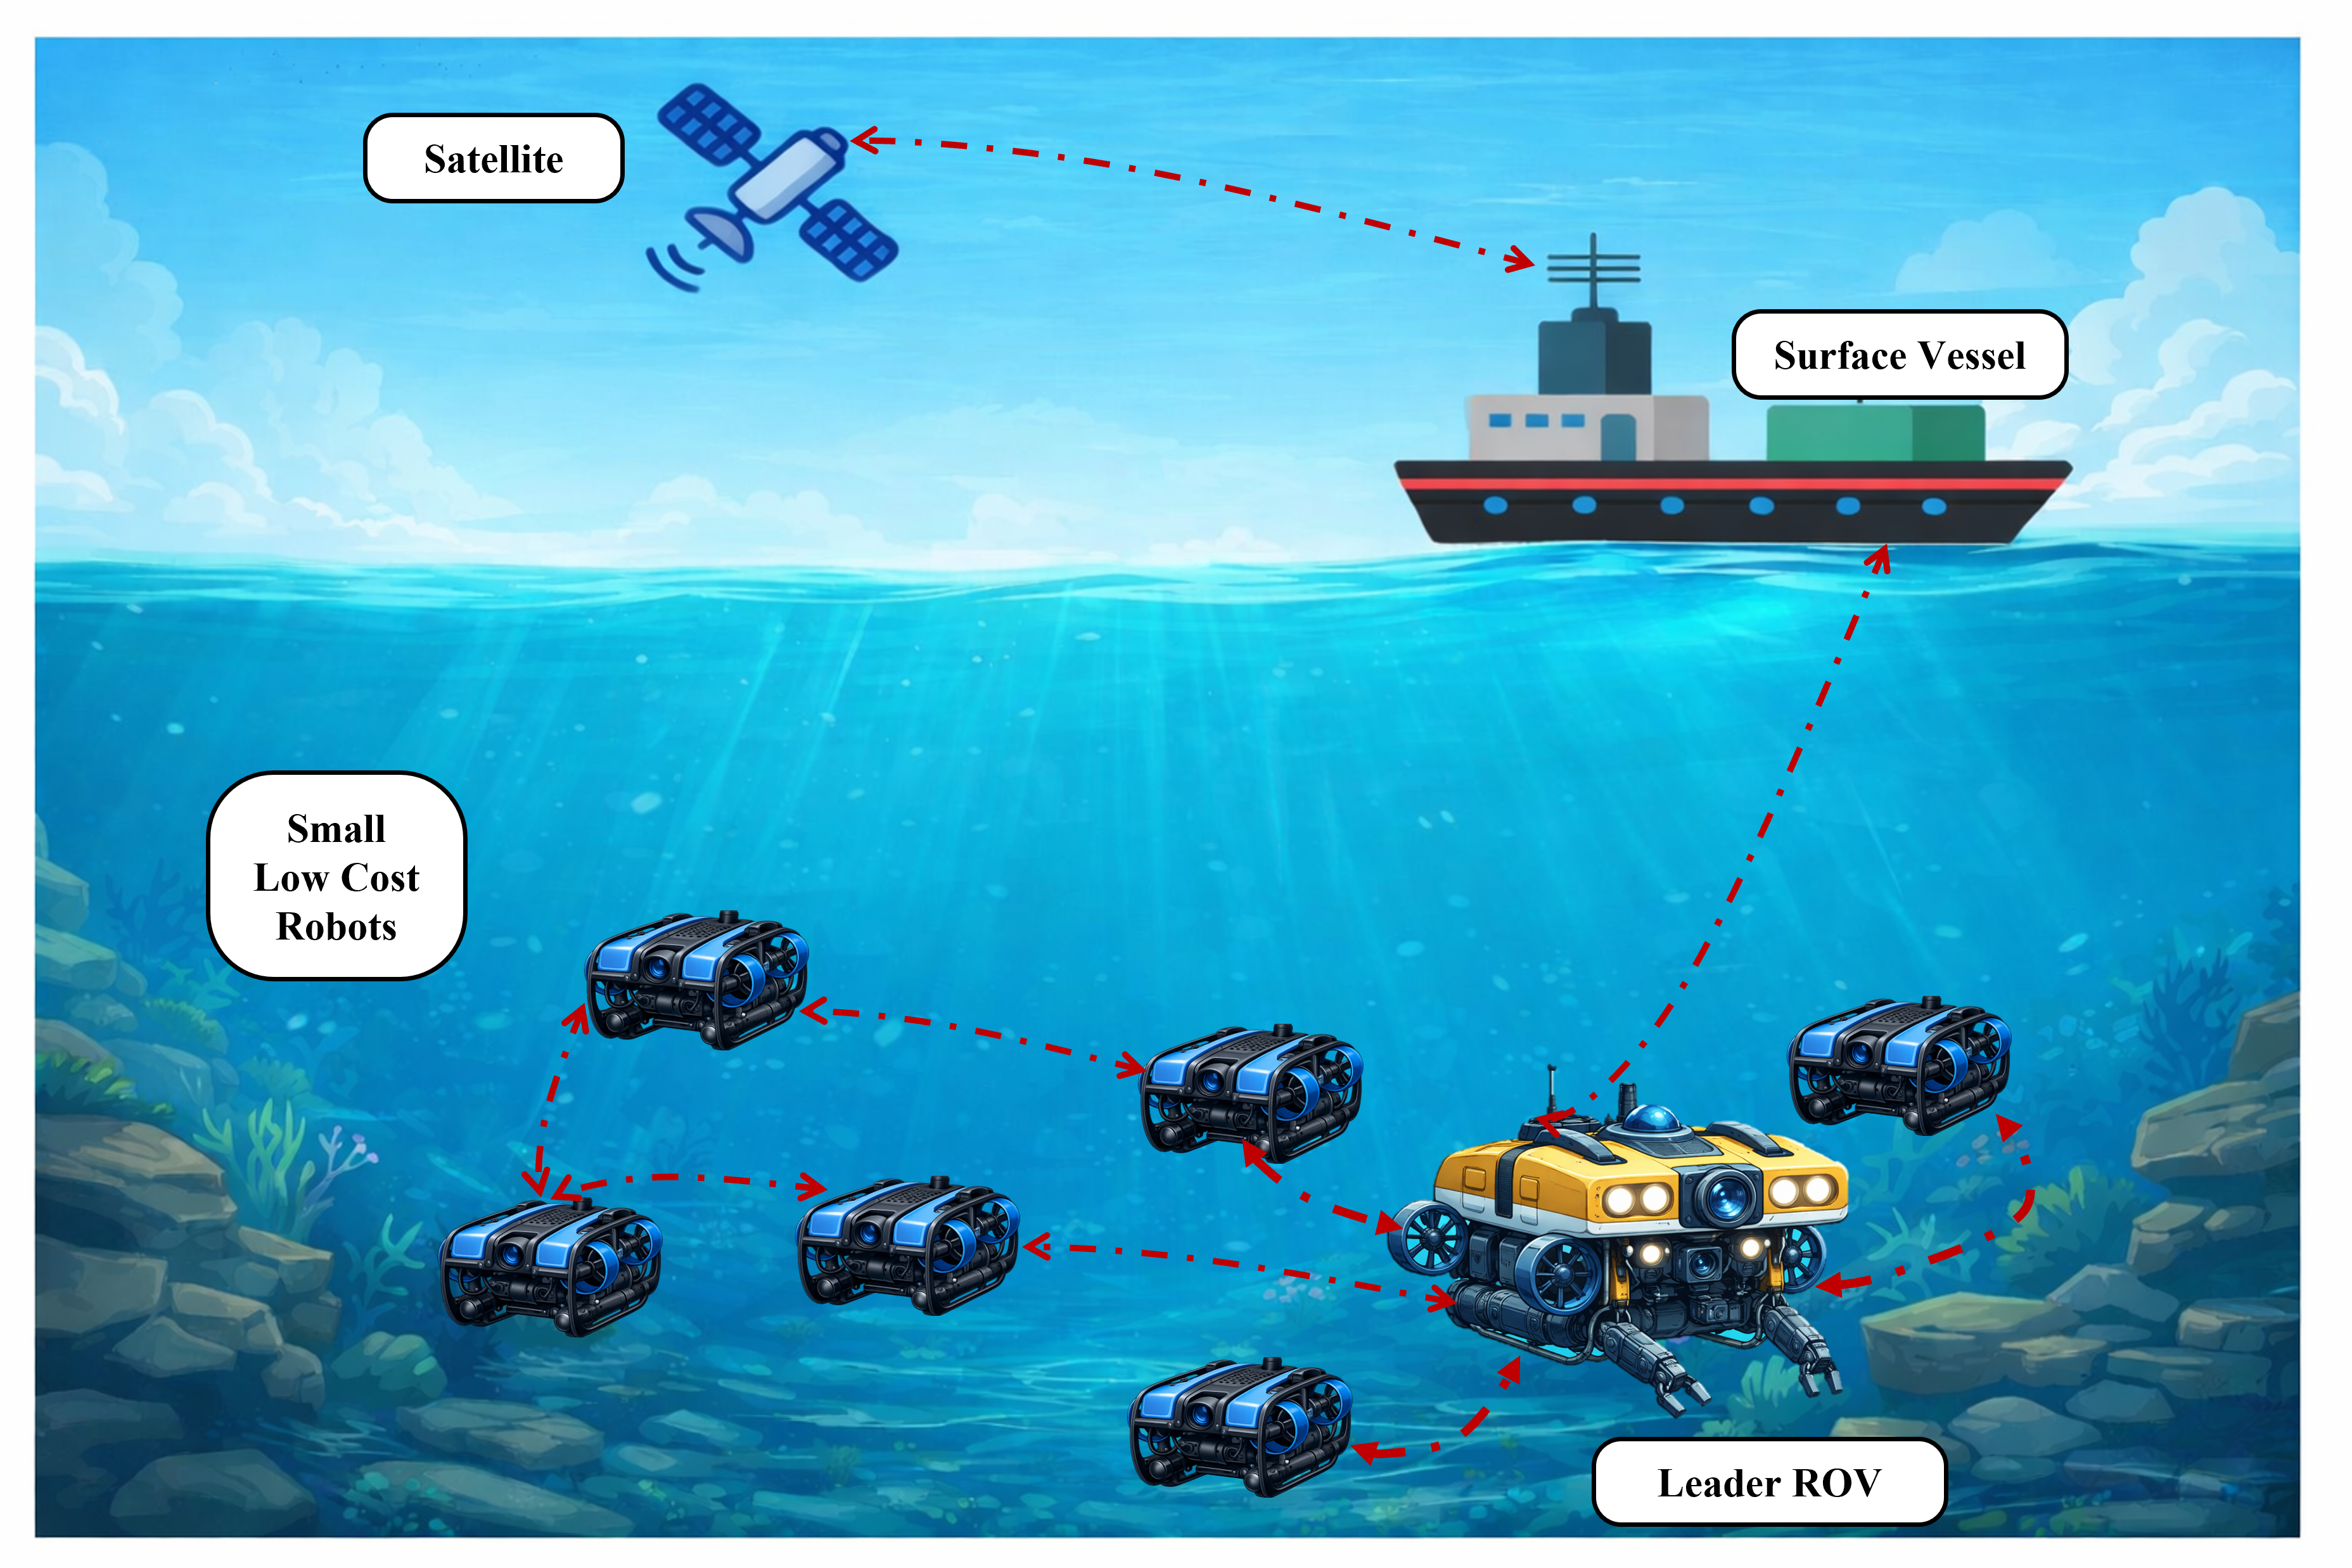
\includegraphics[width=0.95\linewidth]{fig/Scheme.png}
\caption{Concept configuration of the proposed framework for underwater swarm robots. The dotted lines represent the communication links.}
\label{fig:concept}
\end{figure}
Acoustic positioning remains the most established and widely used approach for underwater localization. Classical long-baseline (LBL), short-baseline (SBL), and ultra-short-baseline (USBL) systems estimate position from acoustic time-of-flight, time-difference-of-arrival, or bearing measurements, and they can provide accurate localization over ranges that are difficult to achieve with electromagnetic methods. Moreover, recent developments have significantly reduced the size, cost, and power requirements of acoustic localization hardware. Examples include compact USBL systems, inverted USBL architectures, passive inverted USBL (piUSBL) localization for small AUVs, and low-cost acoustic pseudoranging approaches using MEMS microphones~\cite{Luo2021Review,Rypkema2019piUSBL,Wang2022PassiveIUSBL,Hinduja2022MEMSAcoustic}.

Nevertheless, the requirements of dense swarms of miniature underwater robots introduce a different set of constraints. When localization hardware must be replicated across many agents, the per-agent cost, volume, power consumption, synchronization requirements, acoustic-channel sharing, and update-rate limitations become important design considerations. Acoustic methods may also suffer from multipath and reverberation in confined or shallow-water environments. Therefore, the objective of this work is not to replace modern acoustic positioning systems, but to investigate a complementary short-range relative-localization modality for compact underwater agents. In particular, we explore whether Sub-GHz RF received signal strength measurements, combined with antenna directivity and IMU information, can provide useful local relative-position estimates over short ranges where compactness, low hardware complexity, and swarm scalability are critical.

Localization systems are generally divided into two main categories: range-free and range-based. Range-free techniques depend on network connectivity and usage patterns, whereas range-based techniques rely on estimating distances or angles between nodes. From an application standpoint, range-based methods can be further divided into Global Positioning and Local Positioning. The aim of this research is to develop a framework that enables agents within a swarm to determine their positions relative to one another and, in particular, relative to a designated leader agent with superior sensing capabilities. Local positioning approaches are further classified into self-positioning and remote positioning, with additional details available in~\cite{zekavat2019handbook}. In this work, the primary emphasis is on self-positioning of the agents with respect to the leader agent.

From an operational standpoint, range-based localization methods primarily rely on received signal characteristics, including: (1) Time of Arrival (ToA), (2) Time Difference of Arrival (TDoA), (3) Direction of Arrival (DoA), and (4) Received Signal Strength Indicator (RSSI). In general, ToA, TDoA, and DoA assume Line-of-Sight (LoS) communication, whereas RSSI can also function under non-LoS conditions, albeit typically with reduced performance and accuracy compared with unobstructed scenarios. In addition, ToA and TDoA techniques demand highly accurate time synchronization between transmitter and receiver. While such synchronization is mature and widely used in acoustic systems, it becomes difficult to implement in RF systems, since electromagnetic waves propagate at the speed of light and the relevant distances are on the order of meters. Consequently, DoA and RSSI are usually the only feasible choices for RF-based localization and are well documented in the literature for in-air localization \cite{Tomic2019,Ketabalian2020,Wu2024}. Prior work has demonstrated that antenna directivity can be leveraged for both localization \cite{Jiang2013} and orientation estimation \cite{Wielandner2021}. Note that most existing systems operate at 2.4 GHz or, more recently, at 5 GHz RF bands. RSSI- and DoA-based approaches have also been investigated and validated in underwater environments~\cite{Sathish2023,Luo2021Review}, but typically in conjunction with multiple anchored nodes using acoustic links or magnetic induction~\cite{Garcia2020}. In contrast, the present research targets underwater localization using Sub-GHz RF signals, exploiting DoA and RSSI at these lower frequencies—an area that remains largely unexplored, apart from the concept previously introduced by the authors in \cite{Masood2025}.
\begin{table}
\centering
\caption{Comparison of Basic Localization Methods \cite{zekavat2019handbook}}
\label{tab:comparisonliterature}
\begin{tabularx}{0.4\textwidth}{lccc}
\toprule
\textbf{Method} & \textbf{Accuracy} \footnotemark[1] & \textbf{LOS} & \textbf{Base Station(s)} \\
\midrule
ToA & M & Yes & $\leq3$ \\
TDoA & M & Yes & $\geq3$ \\
DoA & L & Yes & $\geq2$ \\
RSSI & H & No & $\geq3$ \\
\bottomrule
\end{tabularx}
\end{table}
\footnotetext[1]{Scale for Accuracy: L = Low, M = Medium, H = High}

At low RF frequencies, phase-based direction-of-arrival (DoA) estimation becomes impractical because the large wavelength demands wide antenna spacing to obtain sufficiently distinct phase differences. The phase offset between two antennas separated by a distance $d_a$ is given by $\Delta\phi = \frac{2\pi d_a}{\lambda} \sin\theta$. In phased-array systems such as Bluetooth DoA, the antenna spacing is typically set to about $\lambda/2$ to maximize phase sensitivity while preventing spatial aliasing. At 433 MHz, the wavelength is approximately $\lambda \approx 0.69$ m, leading to an optimal inter-element spacing of $\lambda/2 \approx 0.345$ m. For a standard 8-element linear array used in DoA estimation, this yields a total aperture of $L = (N-1)d_a = 7 \times 0.345 \approx 2.4\,\text{m}$. An array extending over more than two meters is clearly unsuitable for compact robotic platforms. Conversely, if the antenna spacing is reduced to a more practical value such as 10 cm, the maximum achievable phase difference becomes $\Delta\phi_{\max} = \frac{2\pi(0.10)}{0.69} \approx 0.91\,\text{rad} \approx 52^\circ$. This restricted phase variation substantially degrades the resolution and accuracy of DoA estimation, rendering it unreliable for precise localization. Consequently, an alternative approach is needed—one that leverages the inherent directivity of RF signals and employs a circular array of directional antennas to infer the angle of arrival from RSSI differences. Developing and analyzing such a method is the primary focus of this research.

In practice, the antenna’s directivity and radiation pattern deviate from the ideal theoretical model. This method has not been extensively investigated, particularly in underwater environments, and its performance is expected to be inferior to phase-based DoA estimation. However, compared to the commonly used Inertial Navigation System (INS), which relies on integrating acceleration and angular velocity, the proposed approach can achieve better long-term accuracy by reducing the drift inherent to inertial navigation. The proposed framework fuses RF-based localization with IMU-based motion propagation to further enhance the accuracy and robustness of relative localization, while simultaneously mitigating inertial drift. The main contributions of this research are summarized as follows:

\begin{enumerate}
\item Experimentally establish that the Sub-GHz RF signal can be used for underwater communication and localization.
\item Considering the fact that phase-based DoA estimation is impractical at Sub-GHz frequencies, show that the directivity of the RF signal can be used to estimate the angle of arrival based on RSSI differences across a circular array of directional antennas.
\item In the presence of multi-path and other uncertainties, show that a physics-aware learning framework can be used to enhance the localization accuracy by learning the complex relationship between the RSSI measurements and the relative position.
\item Show that fusing the RF-based localization with IMU-based motion propagation can further improve the accuracy and robustness of the relative localization, while mitigating the drift associated with inertial navigation.
\end{enumerate}

%The paper is structured as follows: Section II describes the proposed framework, including the theoretical basis for RF-based localization and the fusion with IMU data. Section III details the hardware design of the localization device and the experimental setup for collection of sensory data and ground truth for training. Section IV presents the training and sensor fusion methods, while Section V discusses the results and performance of the proposed framework. Finally, Section VI concludes the paper and outlines future research directions.

\section{The Framework}
% Describe the framework, the hardware design
The proposed framework leverages the directional characteristics of Sub-GHz radio signals to infer the relative positions of agents in a swarm. Each agent is equipped with a localization module consisting of at least three RF antennas, uniformly spaced in angle within the horizontal plane, thereby targeting a planar localization scenario. The received signal strength indicator (RSSI) measured at these antennas provides the primary information for estimating the relative bearing, denoted as $\theta$, and distance, denoted as $d$, to a transmitting agent. Throughout the paper, the subscript $\mathrm{gt}$ denotes ground-truth quantities obtained from the overhead vision system, and hatted variables denote learned, filtered, or reconstructed estimates. The analytical RSS/AoA intermediate quantities are denoted as $d_{\mathrm{RSS}}$ and $\theta_{\mathrm{AoA}}$ without hats. The theoretical development in this section therefore focuses on the RSSI-based localization principle. In the practical implementation, auxiliary magnetometer and gyroscope measurements are used during the learning and correction stages to improve orientation consistency and relative position reconstruction. The complete processing pipeline is summarized in Fig.~\ref{fig:system_process}. This section presents the theoretical basis of the RF-based localization approach, subject to the following assumptions:

\begin{figure*}[t]
\centering
\resizebox{\textwidth}{!}{%
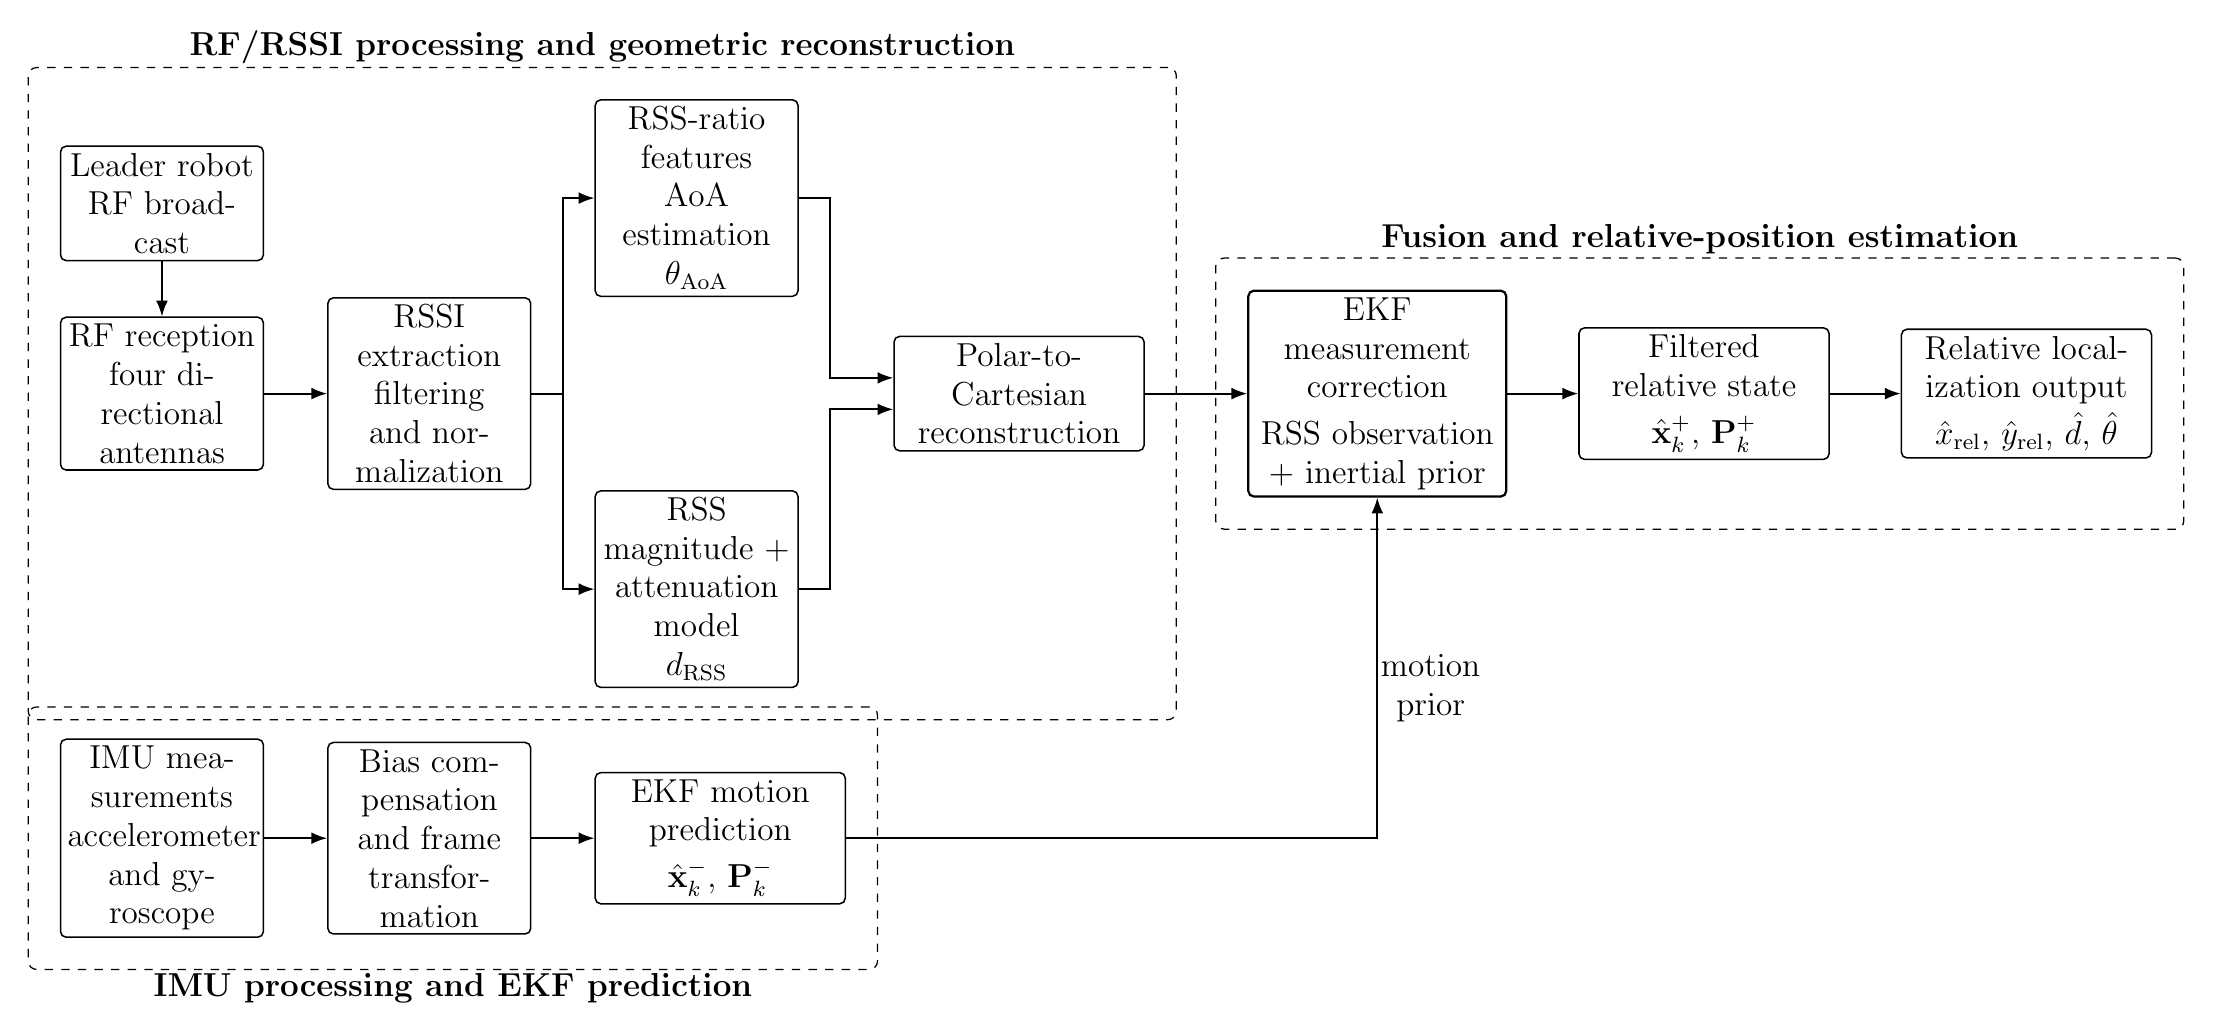
\begin{tikzpicture}[
    font=\large,
    >={Latex[length=2mm]},
    flow/.style={->, line width=0.65pt},
    block/.style={
        draw,
        rounded corners=2pt,
        align=center,
        minimum height=10mm,
        text width=24mm,
        inner sep=2.5pt,
        line width=0.55pt
    },
    wide/.style={
        block,
        text width=30mm,
        minimum height=11mm
    },
    fusion/.style={
        block,
        text width=31mm,
        minimum height=13mm,
        line width=0.8pt
    },
    outputbox/.style={
        block,
        text width=30mm,
        minimum height=11mm
    },
    group/.style={
        draw,
        dashed,
        rounded corners=3pt,
        inner sep=4mm,
        line width=0.45pt
    },
    grouplabel/.style={
        fill=white,
        inner sep=1pt,
        font=\large\bfseries
    },
    edgeLabel/.style={
        font=\large,
        fill=white,
        inner sep=1pt,
        align=center
    }
]

% RF/RSSI processing
\node[block] (rf) {RF reception\\four directional antennas};
\node[block, above=7mm of rf] (leader) {Leader robot\\RF broadcast};
\node[block, right=8mm of rf] (rssi)
{RSSI extraction\\filtering and normalization};

\node[block, above right=0mm and 8mm of rssi] (aoa)
{RSS-ratio features\\AoA estimation\\$\theta_{\mathrm{AoA}}$};

\node[block, below right=0mm and 8mm of rssi] (range)
{RSS magnitude +\\attenuation model\\$d_{\mathrm{RSS}}$};

\node[wide, right=12mm of $(aoa.east)!0.5!(range.east)$] (rsspos)
{Polar-to-Cartesian reconstruction\\[1mm]};

% IMU prediction
\node[block, below=34mm of rf] (imu)
{IMU measurements\\accelerometer and gyroscope};

\node[block, right=8mm of imu] (imuproc)
{Bias compensation\\and frame transformation};

\node[wide, right=8mm of imuproc] (predict)
{EKF motion prediction\\[1mm]
$\hat{\mathbf x}_{k}^{-},\,\mathbf P_{k}^{-}$};

% Fusion and outputs
\node[fusion, right=13mm of rsspos] (correct)
{EKF\\ measurement \\correction\\[1mm]
RSS observation + inertial prior};

\node[outputbox, right=9mm of correct] (state)
{Filtered \\relative state\\[1mm]
$\hat{\mathbf x}_{k}^{+},\,\mathbf P_{k}^{+}$};

\node[outputbox, right=9mm of state] (relative)
{Relative localization output\\[1mm]
$\hat{x}_{\mathrm{rel}},\,\hat{y}_{\mathrm{rel}},\,
\hat{d},\,\hat{\theta}$};

% Data flow
\draw[flow] (leader) -- (rf);
\draw[flow] (rf) -- (rssi);
\draw[flow] (rssi.east) -- ++(4mm,0) |- (aoa.west);
\draw[flow] (rssi.east) -- ++(4mm,0) |- (range.west);
\draw[flow] (aoa.east) -- ++(4mm,0) |- ([yshift=2mm]rsspos.west);
\draw[flow] (range.east) -- ++(4mm,0) |- ([yshift=-2mm]rsspos.west);

\draw[flow] (imu) -- (imuproc);
\draw[flow] (imuproc) -- (predict);

\draw[flow] (rsspos) -- (correct);

\draw[flow] (predict.east) -- ++(7mm,0) -|
node[pos=0.72, right, edgeLabel] {motion\\prior}
(correct.south);

\draw[flow] (correct) -- (state);
\draw[flow] (state) -- (relative);

% Visual grouping
\node[group, fit=(leader)(rf)(rssi)(aoa)(range)(rsspos),
      label={[grouplabel]north:RF/RSSI processing and geometric reconstruction}] {};

\node[group, fit=(imu)(imuproc)(predict),
      label={[grouplabel]south:IMU processing and EKF prediction}] {};

\node[group, fit=(correct)(state)(relative),
      label={[grouplabel]north:Fusion and relative-position estimation}] {};

\end{tikzpicture}
}
\caption{Overview of the proposed RF--IMU relative localization pipeline.}
\label{fig:system_process}
\end{figure*}

\noindent
\begin{itemize}
\item \textbf{Homogeneity of Water:} The RF signal propagates in a homogeneous medium with exponential attenuation.
\item \textbf{Directivity of Antennas:} The directional gain of the patch antennas can be approximated by a quadratic beam model~\cite{Stutzman1998}.
\item \textbf{No Multi-path:} The environment does not introduce significant multi-path reflections that would distort the RSSI measurements.
\item \textbf{Synchronous Measurements:} The RSSI measurements from the multiple antennas are synchronized and can be compared directly to estimate the angle of arrival.
\item \textbf{IMU Accuracy:} The IMU provides accurate measurements of linear acceleration and angular velocity, which can be integrated to estimate motion between RF-based updates.
\end{itemize}


The assumptions listed above are required for the theoretical model to function, but they may not be valid in real-world settings. After presenting the theoretical model, we will concentrate on practical challenges and demonstrate how the proposed framework can alleviate these issues to achieve improved localization performance in practical environments.

As discussed in the literature (Table \ref{tab:comparisonliterature}), localization techniques such as RSSI and DoA typically require at least two base stations. In other words, the agent must receive RF signals from a minimum of two antennas in order to estimate its relative position in a planar scenario. By jointly exploiting both RSSI and DoA, we demonstrate that the proposed framework can deliver localization estimates using only a single reference node, which in this context is the transmitting agent. In addition, the framework is intended for application in swarm formation control, where multiple transmitting agents may be present. This configuration can further improve localization accuracy and robustness by supplying measurements from several directions. For now, the research is primarily concerned with establishing the framework and validating it with a single transmitting agent, while the extension to scenarios with multiple transmitting agents is left for future work.

Consider a transmitting agent (located at $(x_t, y_t)$) that emits an RF signal, which is captured by multiple directional antennas mounted on a receiving agent (placed at $(x_r, y_r)$ and oriented at angle $\psi$ in the world frame). For the receiving agent to determine its own position and orientation in the world frame, it requires the following information:
\begin{enumerate}
\item \textbf{Transmitting Agent Position:} The position of the transmitting agent is denoted by $(x_t, y_t)$.
\item \textbf{World Frame Orientation $\psi$:} The ground-truth yaw angle is denoted by $\psi_{\mathrm{gt},k}$, and its estimate $\hat{\psi}_k$ can be obtained from magnetometer measurements and further fused with gyroscope data to provide a more accurate and stable heading estimate. Even though the receiving agent can estimate the relative bearing to the transmitting agent, estimating its own orientation strengthens the bearing-angle reconstruction.
\item \textbf{Distance $d$:} The ground-truth distance between the transmitting and receiving agent is denoted by $d_{\mathrm{gt},k}$, and its final estimate $\hat{d}_k$ is obtained from RSSI-based learning, which is the main focus of this research.
\item \textbf{Relative Bearing $\theta$:} The ground-truth relative bearing from the receiving agent to the transmitting agent is denoted by $\theta_{\mathrm{gt},k}$, and its final estimate $\hat{\theta}_k$ is obtained from RSSI measurements across the multiple directional antennas, which is also a main focus of this research.
\end{enumerate}

Once the above information is available, the receiving agent can determine its relative position simply by solving the corresponding geometric relations. The estimated receiver position relative to the transmitter frame is denoted by $(\hat{x}_{\mathrm{rel},k},\hat{y}_{\mathrm{rel},k})$, while the reconstructed absolute receiver position is denoted by $(\hat{x}_k,\hat{y}_k)$. These quantities are computed as
\begin{equation}
\begin{bmatrix}\hat{x}_{\mathrm{rel},k} \\
\hat{y}_{\mathrm{rel},k}\end{bmatrix}
= -\hat{d}_k \begin{bmatrix}\cos(\hat{\psi}_k + \hat{\theta}_k) \\
\sin(\hat{\psi}_k + \hat{\theta}_k)\end{bmatrix},
\qquad
\begin{bmatrix}\hat{x}_k \\
\hat{y}_k\end{bmatrix}
= \begin{bmatrix}x_t \\
y_t\end{bmatrix}
+ \begin{bmatrix}\hat{x}_{\mathrm{rel},k} \\
\hat{y}_{\mathrm{rel},k}\end{bmatrix}.
\label{eqn:position}
\end{equation}

\subsection{Orientation in World Frame}
Consider the sample at index $k$, where the sensor readings are given by $\mathbf{m}_k = [m_{x,k}, m_{y,k}]^T$ for the 2D magnetometer measurement in the plane, $\omega_k$ for the gyroscope yaw rate, and $t_k$ for the timestamp associated with sample $k$. The goal is to recover the ground-truth yaw angle $\psi_{\mathrm{gt},k} \in [0,2\pi)$. The corresponding yaw estimate is represented by $\hat{\psi}_k$.

\subsubsection{Gyroscope Based}
The gyroscope-only yaw estimate is obtained by bias-corrected integration of the measured yaw rate. Let
\begin{equation}
\Delta t_k =
\begin{cases}
0, & k=0,\\
t_k - t_{k-1}, & k\ge 1,
\end{cases}
\end{equation}
where \(t_k\) denotes the sample timestamp in seconds. The bias-corrected angular velocity is
\begin{equation}
\tilde{\omega}_k = \omega_k - b_g,
\end{equation}
where \(b_g\) denotes the gyroscope bias obtained from the training data. The incremental change in yaw is given by \(\Delta \psi_k = \tilde{\omega}_k \Delta t_k\).
Therefore, the updated yaw estimate becomes
\begin{equation}
\hat{\psi}^{(\omega)}_k
=
\hat{\psi}^{(\omega)}_{k-1} + \Delta \psi_k,
\end{equation}
with initialization $\hat{\psi}^{(\omega)}_0 = \psi_{\mathrm{gt},0}$.
Equivalently, the estimate may be written as
\begin{equation}
\hat{\psi}^{(\omega)}_k
=
\psi_{\mathrm{gt},0} + \sum_{i=1}^{k} (\omega_i - b_g)\Delta t_i.
\end{equation}
\textbf{Note:} The gyroscope-based estimate does need an initial ground-truth angle $\psi_{\mathrm{gt},0}$ to initialize the integration.

\subsubsection{Magnetometer Based}
The magnetometer-based yaw estimate is obtained directly from the planar magnetometer measurements:
\begin{equation}
\hat{\psi}_k^{(m)} = \operatorname{atan2}(m_{y,k}, m_{x,k}).
\label{eq:mag_heading_direct}
\end{equation}
While \eqref{eq:mag_heading_direct} provides a direct estimate of yaw, in practice the magnetometer measurements are often affected by hard-iron bias, soft-iron distortion, scale mismatch, and environmental magnetic disturbances. Therefore, instead of relying only on the raw heading computed from the planar components, a learning-based mapping is introduced to estimate orientation from magnetometer-derived features.

To improve robustness, a feature vector is constructed from the planar magnetometer measurements as
\begin{equation}
\mathbf{x}^{(m)}_k =
\begin{bmatrix}
m_{x,k} \\
m_{y,k} \\
r_k \\
\cos \varphi_k \\
\sin \varphi_k
\end{bmatrix},
\end{equation}
where $r_k = \sqrt{m_{x,k}^2 + m_{y,k}^2}$ denotes the magnetometer magnitude and \(\varphi_k = \operatorname{atan2}(m_{y,k},m_{x,k})\) is the direct magnetometer heading. The inclusion of both raw and transformed features allows the estimator to exploit not only the measured field components but also their magnitude and directional structure.

Because yaw is an angular variable with \(2\pi\)-periodicity, direct regression of the angle may introduce discontinuities near the wrap-around boundary. To avoid this issue, the target yaw angle \(\psi_{\mathrm{gt},k}\) is represented in cosine-sine form as
\begin{equation}
\mathbf{y}_k =
\begin{bmatrix}
\cos \psi_{\mathrm{gt},k} \\
\sin \psi_{\mathrm{gt},k}
\end{bmatrix}.
\end{equation}

A multilayer perceptron (MLP) regressor is then used to learn the nonlinear mapping
\begin{equation}
\hat{\mathbf{y}}_k^{(m)} = f_m\!\left(\mathbf{x}^{(m)}_k;\Theta_m\right),
\end{equation}
where \(\Theta_m\) denotes the trainable parameters of the network. For a two-hidden-layer MLP, this mapping may be written as
\begin{equation}
\hat{\mathbf{y}}_k^{(m)}
=
\mathbf{W}_3 \,
\sigma\!\Bigl(
\mathbf{W}_2 \,
\sigma\!\left(
\mathbf{W}_1 \mathbf{x}^{(m)}_k + \mathbf{b}_1
\right)
+ \mathbf{b}_2
\Bigr)
+ \mathbf{b}_3,
\label{eqn:MLPEquation}
\end{equation}
where \(\mathbf{W}_i\) and \(\mathbf{b}_i\) are the weight matrices and bias vectors, respectively, and \(\sigma(\cdot)\) is the nonlinear activation function.

Finally, the predicted yaw angle is recovered from the network output using
\begin{equation}
\hat{\psi}_k^{(m,\mathrm{MLP})}
=
\operatorname{atan2}\!\left(\hat{y}_{k,2}^{(m)}, \hat{y}_{k,1}^{(m)}\right),
\end{equation}
where \(\hat{y}_{k,1}^{(m)}\) and \(\hat{y}_{k,2}^{(m)}\) denote the predicted cosine and sine components, respectively.

\subsection{Direction of Arrival (DoA)}
Before we estimate the distance, it is important to estimate the direction of arrival (DoA) accurately, which would enhance the estimation of the distance. Consider a transmitting agent emitting an RF signal which is received by multiple directional antennas on the receiving agent (or multiple receivers). 
The received power at the receiving antenna can be modeled as
\begin{equation}
P_r = P_t + G_t + G_r(\theta) - L(d),
\end{equation}
where $P_t$ is known transmitted power, $G_t$ is also known gain of the transmitting antenna, $G_r(\theta)$ is the gain of the receiving antenna as a function of the angle of arrival $\theta$, and $L(d)$ is the path loss as a function of distance $d$. The powers and gains are typically expressed in decibels (dB), and the path loss is a positive quantity representing the attenuation of the signal.

Assuming exponential attenuation in porous media, the path loss can be approximated as~\cite{vk5br1987}
\begin{equation}
L(d) = \alpha_\omega \times d,
\end{equation}
where $\alpha_\omega$ is the attenuation coefficient (dB/m), dependent on frequency and medium conductivity.
The directional gain pattern of each antenna is approximated by a quadratic beam model~\cite{stutzman2012antenna}
\begin{equation}
G_r(\theta) = G_{\max} - 12\left(\frac{\theta}{\alpha_b}\right)^2,
\end{equation}
where $\alpha_b$ is the half-power beam-width, and $G_{\max}$ is the maximum gain at the boresight. The gain decreases quadratically as the angle deviates from the boresight, with a rate determined by the beam-width.

The direction of arrival (DoA), denoted by $\theta$, is defined in the receiver agent’s body frame. The received signal strength at each antenna in the array is represented by $S_{r,i}, S_{r,j}, S_{r,k}, \dots$, where $i$ indexes the antenna with the highest received power, and $j, k, \dots$ refer to neighboring antennas in the direction of the second-highest signal strength. As stated previously, the antennas are uniformly spaced in azimuth on the horizontal plane, so the boresight of antenna $i$ is given by $\theta_i = i \times 360^\circ/N$, where $N$ is the total number of antennas. 

In principle, by comparing RSSI values of adjacent antennas, the difference $\Delta S = S_{r,i} - S_{r,j}$ encodes the relative angle within the coverage sector of antenna $i$. The bearing estimate, expressed relative to the boresight of antenna $i$, is then reconstructed as
\begin{equation}
\theta_{\mathrm{rel}} = -\frac{1}{2} \left( 90^\circ + \frac{\alpha_b}{90^\circ} \frac{\Delta S}{12} \right),
\end{equation}
which leads to the analytical AoA quantity in the body frame as
\begin{equation}
  \theta_{\mathrm{AoA}} = \theta_i + \theta_{\mathrm{rel}} \left( i - j \right).
\end{equation}
where $\theta_i$ is the boresight direction of antenna $i$, and $f(\cdot)$ maps power difference to angular deviation.

\subsection{Distance}
Having estimated the DoA, the distance can be estimated by rearranging the path-loss model. The water attenuation coefficient $\alpha_\omega$ is a function of frequency of the RF signal, the salinity, and the temperature of the water, which is lumped as follows:
\begin{equation}
  \alpha_\omega = 0.0173 \sqrt{f_{rf} \times \sigma},
\end{equation}
where $f_{rf}$ is the frequency of the RF signal in Hz, and $\sigma$ is the conductivity of the water in S/m. For example, for a Sub-GHz RF signal at 433 MHz, and typical fresh water conductivity of 0.01 S/m, the attenuation coefficient is approximately $\alpha_\omega \approx 0.0173 \sqrt{433 \times 10^6 \times 0.01} \approx 36$ dB/m.

The distance can be estimated by rearranging the path-loss model as follows:
\begin{equation}
  d_{\mathrm{RSS}} = \left\lVert \frac{(P_t)_{dB} + (G(\theta_{\mathrm{rel}}))_{dB} - (S_{i})_{dB}}{0.0173\sqrt{f_{rf}} \times \sigma} \right\rVert.
\end{equation}
Using Eq.~\eqref{eqn:position}, the relative position can now be estimated.

\section{Hardware Design}
The localization device consists of four flat patch antennas which are geometrically  arranged around the body-frame at known angles of $90^\circ$ relative to each other. The device also integrates a 9-axes IMU for motion sensing. The entire assembly is packed into a watertight enclosure with a flange sealing, and penetrators for the USB and power connections. The device is compact, lightweight, and waterproofed for underwater deployment as shown in Fig.~\ref{fig:hardware}.
\begin{figure}[t]
\centering
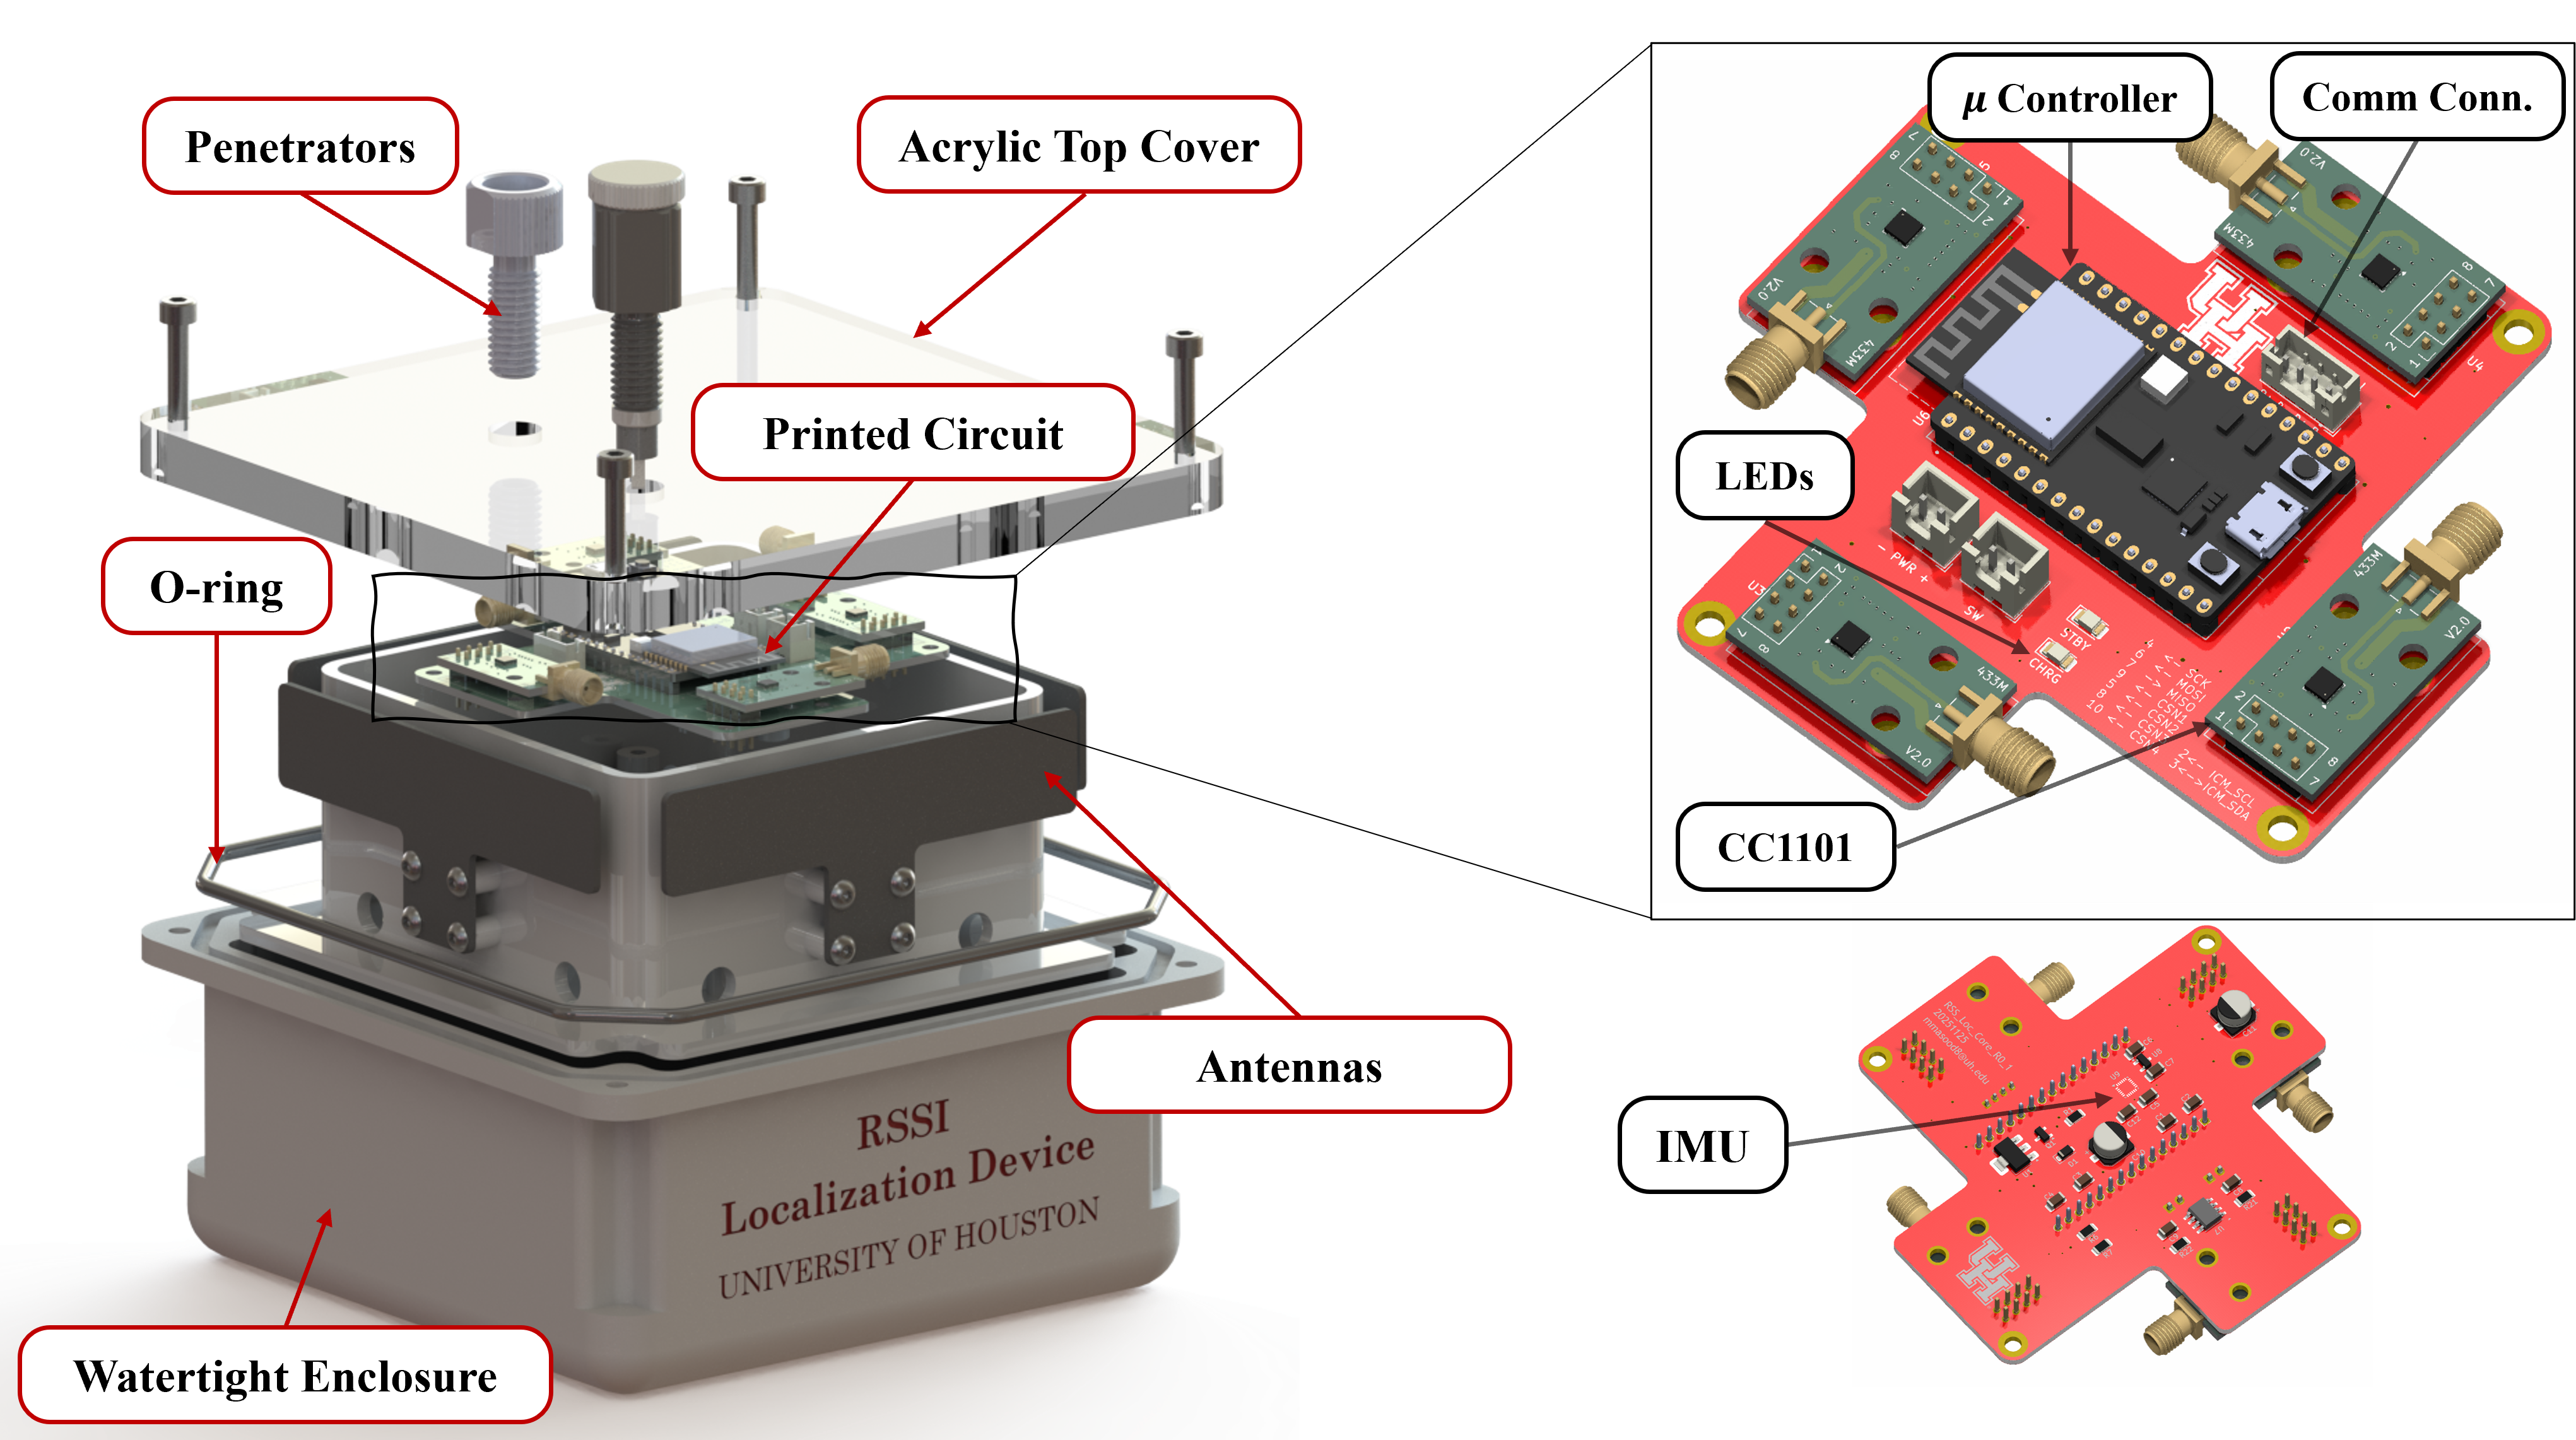
\includegraphics[width=0.48\textwidth]{fig/Device-Description.png}
\caption{Localization device with four flat dipole RF antennas and integrated 9-axes IMU.}
\label{fig:hardware}
\end{figure}

A custom PCB is developed to interface the antennas with a microcontroller that processes the RSSI data and IMU readings. Sub-GHz radio module from Texas Instruments CC1101 is used along with a flat patch antenna from Taoglas. The flat patch antenna is has gain lobes extending in the horizontal plane, symmetric about the boresight. For the purpose of this research, the radiation patterns is required to be antisymmetric in the horizontal plane, to be able to estimate the angle of arrival. This requires the modification of the antenna radio pattern. In the design process, there are two options to achieve this.

\subsection{Directional Sub-GHz Antenna}
% Write informaiton about topologies of antenna and their sizes as per the wavelength.
Sub-GHz frequencies have longer wavelengths (e.g., 433 MHz corresponds to a wavelength of approximately 69 cm), which poses challenges for compact antenna design. The most common antenna types include:
\begin{itemize}
\item \textbf{Half-wave dipole:} Simple design but requires a length of about $\lambda/2$ (34.5 cm), which is too large for compact applications. Perfectly omnidirectional in azimuth.
\item \textbf{Monopole:} Similar to dipole but requires a ground plane. Relatively compact than dipole as the size can be $\lambda/4$ (17.25 cm), but still large for small robots. Omnidirectional in azimuth.
\item \textbf{Patch antenna:} Can be designed to be compact (e.g., 10-15 cm) by using high dielectric substrates. The radiation pattern can be shaped to have directional lobes, but the lobes are typically symmetric about the boresight. The gain is generally lower than dipole or monopole.
\item \textbf{Yagi-Uda:} Directional antenna with multiple elements, but the size can be large (e.g., 30-50 cm) due to the need for multiple elements spaced at $\lambda/4$ intervals.
\end{itemize}
The design choice is a trade-off between size, gain, and directionality.

\subsection{Modified Radiation Pattern}
To create a directional lobe in the horizontal plane while maintaining compact size, the radiation pattern of a dipole antenna can be modified using three approaches: (1) a \textbf{reflector} placed $\lambda/4$ behind the element for constructive interference, requiring dimensions of $\lambda/4$--$\lambda/2$ (17--35 cm) that are impractical for small robots; (2) an \textbf{absorber} made of high-loss material (e.g., ferrite or carbon foam) to suppress unwanted lobes with minimal size increase but at some gain cost; or (3) a \textbf{non-symmetric ground plane} that redirects energy asymmetrically, offering the most compact solution (~3--4 dB front-to-back shift with a same-size metal plate).

For this work, the absorber and non-symmetric ground plane approaches are combined: a 3M AB6005S RF absorber sheet suppresses the back lobe, while a Laird ferrite sheet forms the asymmetric ground plane. The result is a compact modified antenna achieving at least 10 dB front-to-back difference in the azimuth plane.
\subsection{Inertial Measurement Unit}
A 9-axes IMU from TDK InvenSense (ICM-20948) is integrated into the localization device to provide motion sensing capabilities. The IMU includes a 3-axes magnetometer is separately integrated onto the same package in ICM-20948. The IMU data is polled synchronously with the RF signal receiving event in the microcontroller. Remember, the communication between the RF transmitter and receiver may be intermittent, which brings a challenge in the location estimation, which would be discussed in the later sections. 
\subsection{Design of Device}
As the main motivation for this research to support underwater swarm for small compact robots, the design of the localization device is focused on being compact, lightweight, and waterproof. The four dipole antennas are arranged in a square configuration. As the length of the antenna is 10 cm, the overall size of the device is approximately 15 cm x 15 cm x 8 cm. An internal structure holds the antennas facing outwards, while keeps the custom designed PCB with the microcontroller and RF module at the center. The 9-axes IMU is integrated on the PCB to provide motion sensing capabilities. The entire assembly is enclosed in a waterproof casing fabricated using Stereolithography (SLA) 3D printing with a resin material. For wiring, pnetrators from Blue Robotics are used to maintain waterproof integrity while allowing electrical connections to the antennas and sensors. The device is designed to be mounted on small robotic platforms, such as underwater drones or surface vehicles, enabling them to localize relative to each other in a swarm formation. Fig.~\ref{fig:hardware} shows the final design of the localization device, highlighting the four PCB dipole antennas and the integrated IMU within the waterproof enclosure.
\subsection{Communication}
On-board hardware is designed only for the raw sensors measurement only i.e. receiving the RF signal, measuring the RSSI, and recording the IMU data. The acquired data is communicated through the USB interface to a computer for processing and training. The communication is not designed for real-time localization, but the framework can be extended to support real-time operation by implementing the RF–IMU fusion algorithm on the microcontroller and using wireless communication (the same Sub-GHz RF communication) to share localization estimates among agents in the swarm.
\subsection{On-board Battery}
Not the main focus of this research, but the device is designed to be powered by a rechargeable lithium-ion battery. The custom PCB includes a power management circuit that regulates the voltage and provides charging capabilities. The battery is selected to provide sufficient runtime for typical underwater missions, while keeping the weight and size within acceptable limits for small robotic platforms.
\subsection{Experimental Setup and Data Collection}
For the validation of the proposed framework, the wireless communication modules were first independently tested in the water tank to ensure proper operation and signal reception. The communication characteristics especially the workable communication range were tested. The receiver was able to receive the signal with noted strength of -108 dBm at a distance of 10 meters when both the transmitter and the proposed device were held at a depth of 0.5 meters. The details of communication setup and performance results are listed in Table~\ref{tab:rf_parameters}. An experimental setup is designed to collect sensory data along with ground truth position data. The localization device is mounted on a BlueROV from BlueRobotics (shown in Fig.~\ref{fig:hardware-mounted}) that can be moved within a controlled environment while the a transmitter is placed at a fixed location. An AprilTag is fixed on the Remotely Operated Vehicle (ROV) to provide ground truth position data through a computer vision system. The ROV is moved in a predefined trajectory while the localization device collects RSSI and IMU data, which are synchronized with the ground truth position for training the physics-aware learning model.

\begin{table*}[t]
    \centering
    \caption{RF communication and localization parameters.}
    \label{tab:rf_parameters}
    \begin{tabular}{lll}
        \hline
        \textbf{Parameter} & \textbf{Symbol} & \textbf{Value} \\
        \hline
        Carrier frequency 
        & $f_c$ 
        & $433.92~\mathrm{MHz}$ \\

        Modulation 
        & -- 
        & GFSK \\

        Nominal data rate 
        & $R_b$ 
        & $1.2~\mathrm{kBaud}$ \\

        Transmit power 
        & $P_t$ 
        & $+10~\mathrm{dBm}$ \\

        Nominal receiver sensitivity 
        & $S_{\min}$ 
        & Approximately $-112~\mathrm{dBm}$ \\

        Packet airtime 
        & $T_{\mathrm{air}}$ 
        & Approximately $93~\mathrm{ms}$ \\

        Maximum tested reception distance 
        & $r_{\mathrm{comm}}$ 
        & $10~\mathrm{m}$ at $0.5~\mathrm{m}$ depth \\

        Evaluated localization range 
        & $r_{\mathrm{loc}}$ 
        & Up to $6~\mathrm{m}$ \\
        \hline
    \end{tabular}
\end{table*}

\begin{figure}
\centering
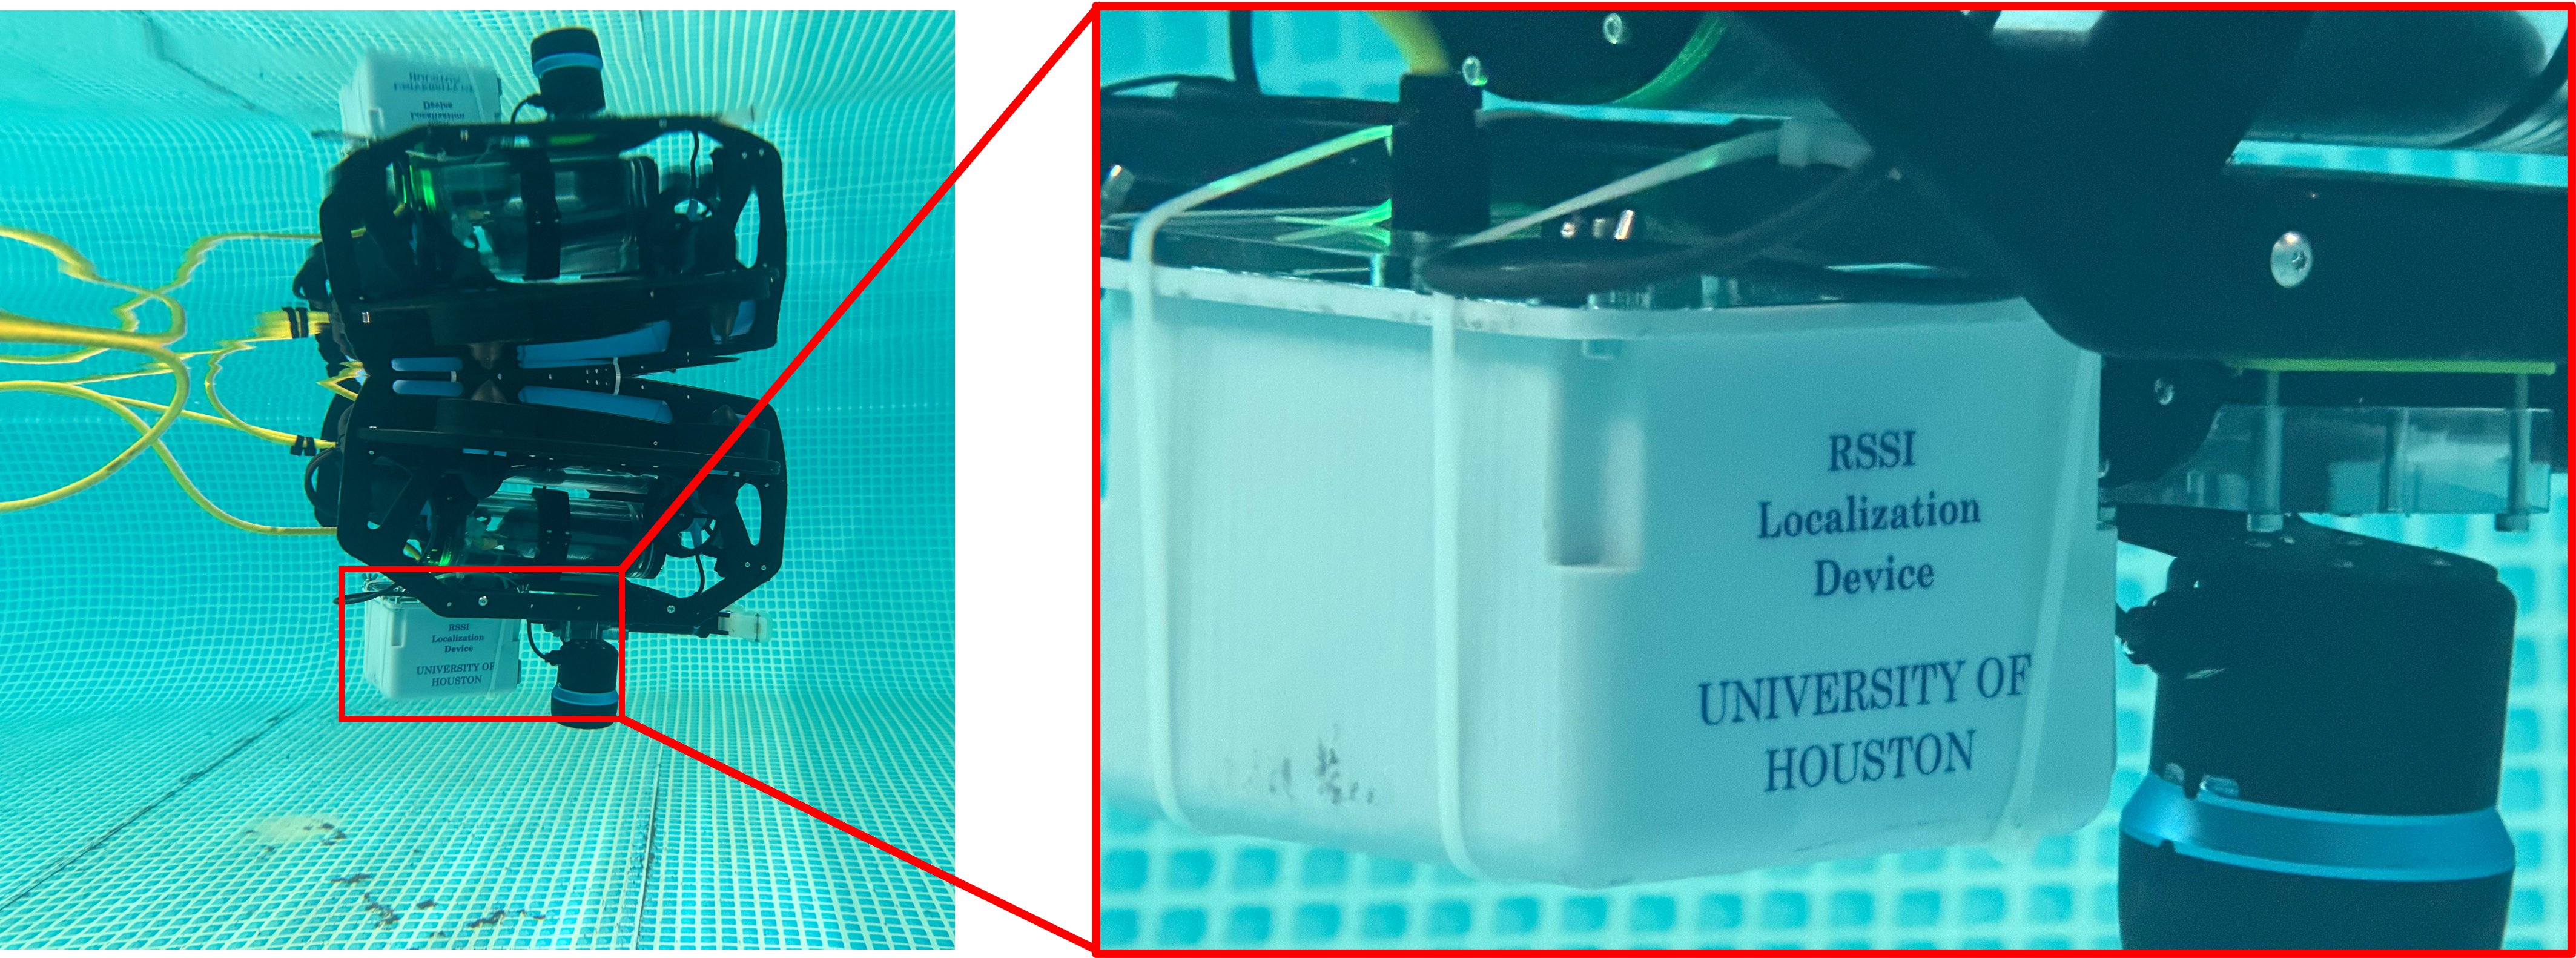
\includegraphics[width=0.48\textwidth]{fig/RSSI-Hardware.png}
\caption{The localization device mounted on BlueROV.}
\label{fig:hardware-mounted}
\end{figure}

\section{Training and Sensor Fusion}
Multiple datasets are collected in the experimental setup, with different working conditions such as different trajectories, different locations of the transmitter antenna. Each dataset contains 19 entries, which are summarized and notated in Table \ref{table:entrieslist}. 
\begin{table*}[ht]
\centering
\caption{Dataset Entries}
\label{table:entrieslist}
\begin{tabular}{lccl}
\toprule
\textbf{Entry} & \textbf{Notation} & \textbf{Description} & \textbf{Units} \\
\midrule
Timestamp (Remote) & $t_k$ & Timestamp recorded at the localization device & seconds \\
Timestamp (Computer) & $t_k^{\mathrm{comp}}$ & Timestamp recorded at the computer for synchronization & seconds \\
RSSI Measurements & $\mathbf{S}_k=[S_{1,k},S_{2,k},S_{3,k},S_{4,k}]^T$ & Received Signal Strength Indicator from 4 antennas & dBm \\
Accelerometer Data & $\mathbf{a}_k$ & 3-axis accelerometer data & m/s$^2$ \\
Gyroscope Data & $\mathbf{\omega}_k$ & 3-axis gyroscope data & rad/s \\
Magnetometer Data & $\mathbf{m}_k$ & 3-axis magnetometer data & $\mu$T \\
Ground Truth Position & $\mathbf{p}_{\mathrm{gt},k}$ & Ground truth position from AprilTag & meters \\
Ground Truth Orientation & $\psi_{\mathrm{gt},k}$ & Ground truth orientation from AprilTag & $^\circ$ \\
\bottomrule
\end{tabular}
\end{table*}

The collected data clearly shows that the theoretical models alone are insufficient in practice due to two key factors:
\begin{enumerate}
  \item \textbf{Multi-path:} In the closed water tank used for data collection, reflections from walls and the waterbed introduce additional signal power that deviates from the analytical path-loss model.
  \item \textbf{Radiation Lobe:} The modified patch antennas do not strictly follow the quadratic beam model and exhibit extra lobes, causing RSSI deviations from theoretical predictions.
\end{enumerate}
% Fig.~\ref{fig:rssi_distance} illustrates the relationship between the measured RSSI and the ground-truth distance. Although an overall decaying trend is evident, the measurements do not follow a simple monotonic distance-only model. In particular, several regions exhibit higher RSSI values than would be expected from a purely exponential attenuation law. These deviations should not be interpreted solely as measurement noise or poor data quality. Rather, they reflect the coupled nature of the sensing process, in which the observed RSSI is influenced not only by propagation distance but also by the direction of arrival, antenna radiation characteristics, and multipath effects.

% Therefore, the RSSI--distance plot should be regarded as a two-dimensional projection of a higher-dimensional physical relationship. Samples acquired at similar distances may correspond to different angular configurations and hence yield substantially different RSSI values. What appears as scatter or outliers in Fig.~\ref{fig:rssi_distance} may thus represent structured variation induced by the underlying sensing geometry, rather than purely random corruption.
% \begin{figure}[ht]
%   \centering
%   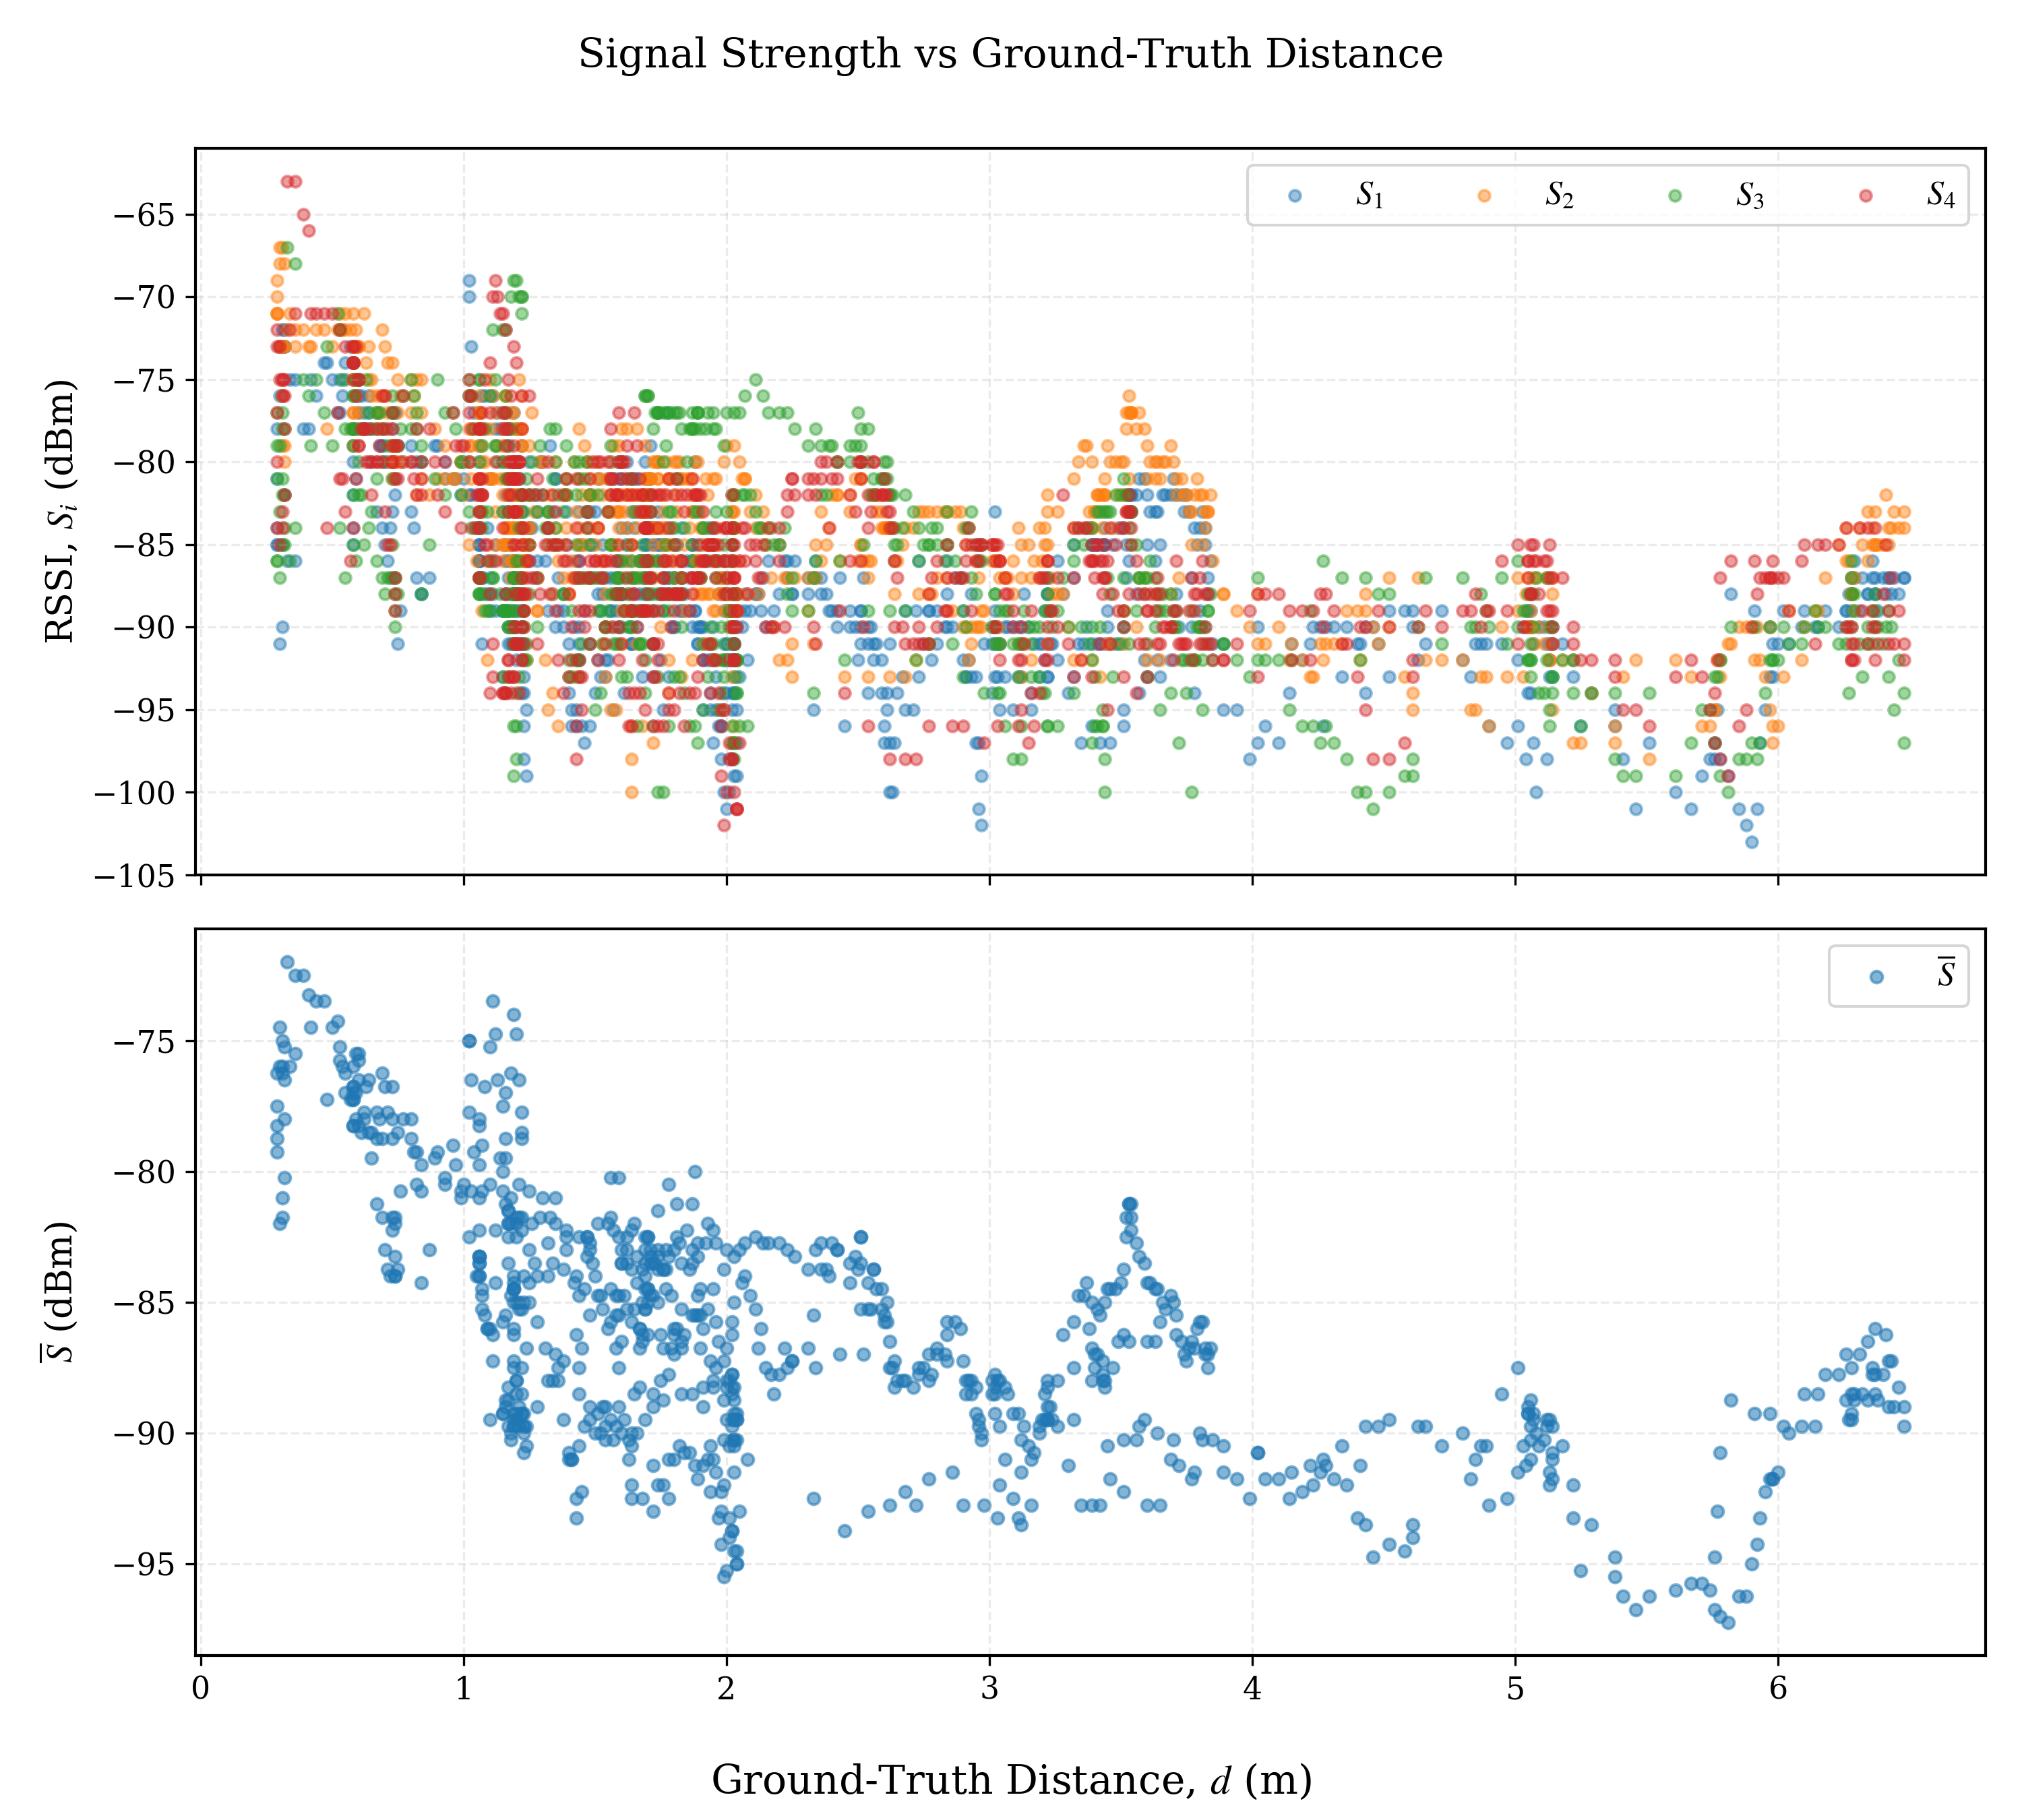
\includegraphics[width=\linewidth]{fig/rssi_vs_distance.png}
%   \caption{Received Signal Strength Indicator (RSSI) measurements as a function of ground truth distance.}
%   \label{fig:rssi_distance}
% \end{figure}
This observation provides the main motivation for adopting a physics-aware learning framework. Instead of forcing a simplified analytical inversion from RSSI to relative position, the proposed approach learns the nonlinear measurement-to-state relationship directly from data, while implicitly accounting for practical effects such as directional gain variation, radiation lobe behavior, and multi-path induced distortions that are difficult to capture explicitly in a closed-form model.

There are following physics-aware rules that can be added to the learning framework to enhance the performance:
\begin{itemize}
  \item \textbf{Circular angle representation:} Angular quantities such as yaw and bearing are represented using sine and cosine components instead of direct angle regression, in order to respect the periodic nature of rotational variables and avoid discontinuities at the wrap-around boundary.
  \item \textbf{Short-horizon gyroscope fusion:} Instead of relying on long-term integration of gyroscope data, which is prone to drift, a short-horizon incremental feature is used to capture recent rotational motion without exposing the estimator to large drift.
  \item \textbf{Feature engineering:} The input feature space is carefully constructed to include not only raw sensor measurements but also derived features.
  \item \textbf{Antenna Asymmetry:} Instead of using raw RSSI values, we can normalize each antenna's RSSI by its own maximum value.
  \item \textbf{Kinematic Continuity:} Knowing the physics of the robot's motion, a continuity condition can be applied. 
\end{itemize}

\subsection{Selection of Training Method}
We started with selection of the training method that can give us the best fitting to the collected data. The purpose of this process is to find the best method that can capture the complex relationship between the sensor measurements and the ground truth target variables, so a single dataset is split into training and testing sets, and nine different models are trained and evaluated on the same data split to ensure a fair comparison. The performance of each model is evaluated based on the coefficient of determination \(R^2\) and the mean absolute error (MAE) in the target variable space. The model that achieves the highest \(R^2\) and lowest MAE on the test set is selected for subsequent experiments and analysis.

Multiple regression methods were tested for orientation, distance, and bearing angle. All candidate models were trained using the same feature representation described in the previous subsection, such that the comparison reflects the regression capability of each method rather than differences in feature construction. In particular, angular targets (yaw and bearing angle) were represented in circular form using their cosine and sine components, and the predicted angle was recovered using the inverse tangent mapping. Due to the periodic nature of angular variables, the estimation error is wrapped as $\operatorname{wrap}(\alpha) = (\alpha+\pi)\bmod 2\pi-\pi$.
% Made with Code test_compare_models_V1.py
% \begin{figure*}[ht]
%   \centering
%   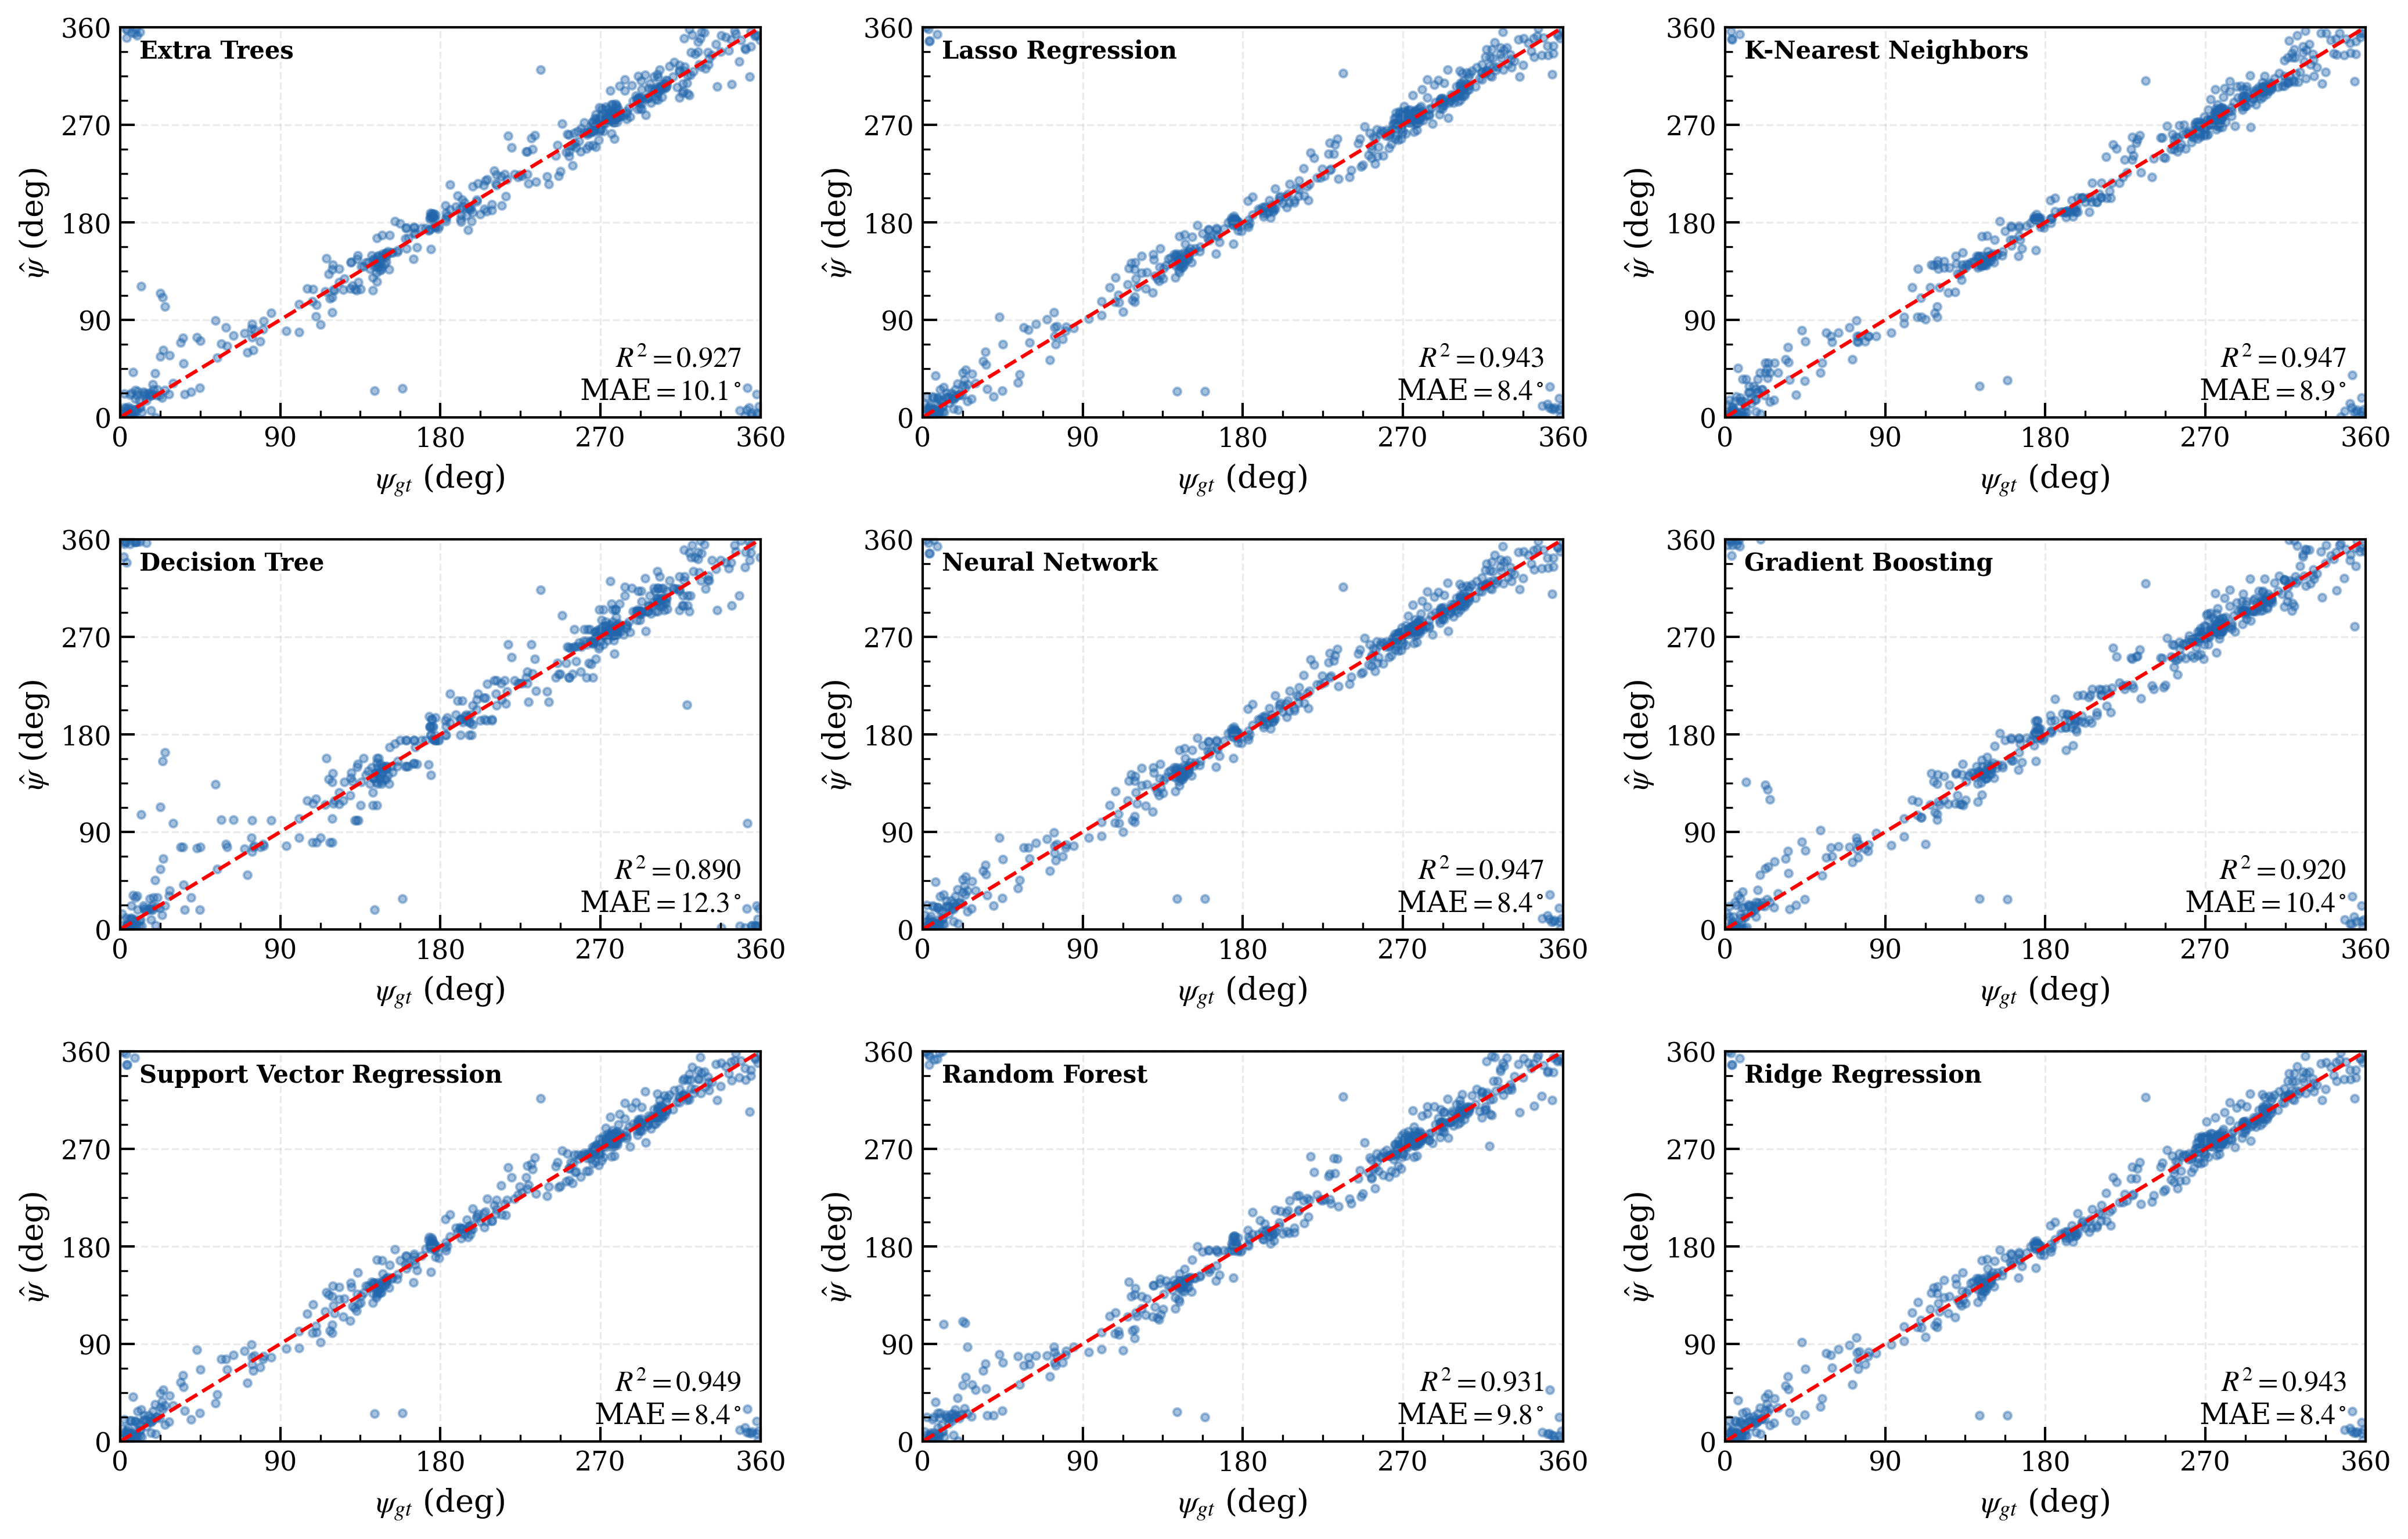
\includegraphics[width=\linewidth]{fig/orientation_model_compare.png}
%   \caption{Comparison of different regression methods for magnetometer-based yaw estimation.}
%   \label{fig:orientation_model_compare}
% \end{figure*}

% for psi orientation
% ================================================================================
% Extra Trees trained and evaluated.
% Extra Trees R^2 (cos/sin): 0.9273 | Mean Abs Angle Error: 10.12 deg
% Lasso Regression trained and evaluated.
% Lasso Regression R^2 (cos/sin): 0.9433 | Mean Abs Angle Error: 8.39 deg
% K-Nearest Neighbors trained and evaluated.
% K-Nearest Neighbors R^2 (cos/sin): 0.9466 | Mean Abs Angle Error: 8.86 deg
% Decision Tree trained and evaluated.
% Decision Tree R^2 (cos/sin): 0.8904 | Mean Abs Angle Error: 12.27 deg
% Neural Network trained and evaluated.
% Neural Network R^2 (cos/sin): 0.9473 | Mean Abs Angle Error: 8.43 deg
% Gradient Boosting trained and evaluated.
% Gradient Boosting R^2 (cos/sin): 0.9205 | Mean Abs Angle Error: 10.39 deg
% Support Vector Regression trained and evaluated.
% Support Vector Regression R^2 (cos/sin): 0.9486 | Mean Abs Angle Error: 8.42 deg
% Random Forest trained and evaluated.
% Random Forest R^2 (cos/sin): 0.9311 | Mean Abs Angle Error: 9.79 deg
% Ridge Regression trained and evaluated.
% Ridge Regression R^2 (cos/sin): 0.9433 | Mean Abs Angle Error: 8.41 deg
% ================================================================================
% For distance based on rssi only
% Extra Trees trained and evaluated.
% Extra Trees R^2: 0.6129 | Mean Abs Error: 0.64 m
% Lasso Regression trained and evaluated.
% Lasso Regression R^2: 0.3456 | Mean Abs Error: 0.97 m
% K-Nearest Neighbors trained and evaluated.
% K-Nearest Neighbors R^2: 0.5217 | Mean Abs Error: 0.78 m
% Decision Tree trained and evaluated.
% Decision Tree R^2: 0.3409 | Mean Abs Error: 0.74 m
% Neural Network trained and evaluated.
% Neural Network R^2: 0.5893 | Mean Abs Error: 0.69 m
% Gradient Boosting trained and evaluated.
% Gradient Boosting R^2: 0.5598 | Mean Abs Error: 0.72 m
% Support Vector Regression trained and evaluated.
% Support Vector Regression R^2: 0.4918 | Mean Abs Error: 0.74 m
% Random Forest trained and evaluated.
% Random Forest R^2: 0.6221 | Mean Abs Error: 0.66 m
% Ridge Regression trained and evaluated.
% Ridge Regression R^2: 0.3457 | Mean Abs Error: 0.97 m
% ================================================================================
% For distance based on rssi and mag
% Extra Trees trained and evaluated.
% Extra Trees R^2: 0.8422 | Mean Abs Error: 0.41 m
% Lasso Regression trained and evaluated.
% Lasso Regression R^2: 0.5262 | Mean Abs Error: 0.85 m
% K-Nearest Neighbors trained and evaluated.
% K-Nearest Neighbors R^2: 0.6655 | Mean Abs Error: 0.65 m
% Decision Tree trained and evaluated.
% Decision Tree R^2: 0.6709 | Mean Abs Error: 0.46 m
% Neural Network trained and evaluated.
% Neural Network R^2: 0.8301 | Mean Abs Error: 0.44 m
% Gradient Boosting trained and evaluated.
% Gradient Boosting R^2: 0.7613 | Mean Abs Error: 0.53 m
% Support Vector Regression trained and evaluated.
% Support Vector Regression R^2: 0.7161 | Mean Abs Error: 0.56 m
% Random Forest trained and evaluated.
% Random Forest R^2: 0.7897 | Mean Abs Error: 0.48 m
% Ridge Regression trained and evaluated.
% Ridge Regression R^2: 0.5293 | Mean Abs Error: 0.84 m

% Estimating angle theta from transmitter:
% Extra Trees trained and evaluated.
% Extra Trees R^2: 0.6574 | Mean Abs Error: 30.23 deg
% C:\Users\mumar\miniconda3\envs\env\Lib\site-packages\sklearn\linear_model\_coordinate_descent.py:716: ConvergenceWarning: Objective did not converge. You might want to increase the number of iterations, check the scale of the features or consider increasing regularisation. Duality gap: 1.791e+05, tolerance: 3.429e+02
%   model = cd_fast.enet_coordinate_descent(
% Lasso Regression trained and evaluated.
% Lasso Regression R^2: 0.4088 | Mean Abs Error: 51.39 deg
% K-Nearest Neighbors trained and evaluated.
% K-Nearest Neighbors R^2: 0.4875 | Mean Abs Error: 43.20 deg
% Decision Tree trained and evaluated.
% Decision Tree R^2: 0.3659 | Mean Abs Error: 37.40 deg
% C:\Users\mumar\miniconda3\envs\env\Lib\site-packages\sklearn\neural_network\_multilayer_perceptron.py:785: ConvergenceWarning: Stochastic Optimizer: Maximum iterations (2000) reached and the optimization hasn't converged yet.
%   warnings.warn(
% Neural Network trained and evaluated.
% Neural Network R^2: 0.5894 | Mean Abs Error: 36.58 deg
% Gradient Boosting trained and evaluated.
% Gradient Boosting R^2: 0.6039 | Mean Abs Error: 35.46 deg
% Support Vector Regression trained and evaluated.
% Support Vector Regression R^2: 0.1248 | Mean Abs Error: 65.95 deg
% Random Forest trained and evaluated.
% Random Forest R^2: 0.6289 | Mean Abs Error: 32.21 deg
% Ridge Regression trained and evaluated.
% Ridge Regression R^2: 0.4080 | Mean Abs Error: 51.51 deg

A similar comparison is performed for distance estimation models as follows:
\begin{equation}
\hat{d}_k = f_d(\mathbf{x}^{(d)}_k;\Theta_d),
\end{equation}
where
\begin{equation*}
\mathbf{x}^{(d)}_k =
\begin{bmatrix}
\mathbf{S}_k \\
m_{x,k} \\ m_{y,k} \\ \|\mathbf{m}_{xy,k}\|_2 \\
\cos\varphi_k \\ \sin\varphi_k
\end{bmatrix},
\quad \mathbf{S}_k = \begin{bmatrix} S_{1,k} \\ S_{2,k} \\ S_{3,k} \\ S_{4,k} \end{bmatrix},
\end{equation*}
with
\begin{equation*}
\|\mathbf{m}_{xy,k}\|_2 = \sqrt{m_{x,k}^2 + m_{y,k}^2},
\qquad
\varphi_k = \operatorname{atan2}(m_{y,k},m_{x,k}).
\end{equation*}

It has been mentioned earlier that the distance information cannot be directly inferred from the RSSI measurements due to the complex coupling with the direction of arrival and antenna radiation pattern. It is observed in the testing as well, and is summarized in Table.~\ref{table:distance_orientation_model_compare} that the best performing model for distance estimation is the Extra Trees, using the clues of absolute orientation $\psi$ indirectly by using the magnetometer features.
\begin{table*}
\centering
\caption{Comparison of different regression methods}
\label{table:distance_orientation_model_compare}
\begin{tabular}{lccccccccc}
\toprule
\multirow{3}{*}{\textbf{Model}}
  & \multicolumn{2}{c}{\textbf{Orientation}}
  & \multicolumn{4}{c}{\textbf{Distance (6m Range)}}
  & \multicolumn{2}{c}{\textbf{Bearing $\theta$}} \\
\cmidrule(lr){2-3}\cmidrule(lr){4-7}\cmidrule(lr){8-9}
  & \multicolumn{2}{c}{Magnetometer}
  & \multicolumn{2}{c}{RSSI Only}
  & \multicolumn{2}{c}{RSSI + Mag}
  & \multicolumn{2}{c}{RSSI + Mag} \\
\cmidrule(lr){2-3}\cmidrule(lr){4-5}\cmidrule(lr){6-7}\cmidrule(lr){8-9}
  & MAE ($^\circ$) & $R^2$ & MAE (m) & $R^2$ & MAE (m) & $R^2$ & MAE ($^\circ$) & $R^2$ \\
\midrule
Extra Trees              & 10.12 & 0.9273 & \underline{0.64} & 0.6129 & \underline{0.41} & 0.8422 & \underline{30.23} & 0.6574 \\
Lasso Regression         &  8.39 & 0.9433 & 0.97 & 0.3456 & 0.85 & 0.5262 & 51.39 & 0.4088 \\
K-Nearest Neighbors      &  8.86 & 0.9466 & 0.78 & 0.5217 & 0.65 & 0.6655 & 43.20 & 0.4875 \\
Decision Tree            & 12.27 & 0.8904 & 0.74 & 0.3409 & 0.46 & 0.6709 & 37.40 & 0.3659 \\
Neural Network           &  \underline{8.43} & 0.9473 & 0.69 & 0.5893 & 0.44 & 0.8301 & 36.58 & 0.5894 \\
Gradient Boosting        & 10.39 & 0.9205 & 0.72 & 0.5598 & 0.53 & 0.7613 & 35.46 & 0.6039 \\
Support Vector Regression&  8.42 & 0.9486 & 0.74 & 0.4918 & 0.56 & 0.7161 & 65.95 & 0.1248 \\
Random Forest            &  9.79 & 0.9311 & 0.66 & 0.6221 & 0.48 & 0.7897 & 32.21 & 0.6289 \\
Ridge Regression         &  8.41 & 0.9433 & 0.97 & 0.3457 & 0.84 & 0.5293 & 51.51 & 0.4080 \\
\bottomrule
\end{tabular}
\end{table*}
\subsubsection{Short-Horizon Gyro-Augmented Magnetometer Yaw Estimator}
To leverage the complementary strengths of the gyroscope and magnetometer, a short-horizon fusion approach is adopted. The gyroscope provides smooth estimates over short time intervals but suffers from long-term drift, while the magnetometer offers absolute heading information but can be noisy and distorted. By fusing these two sources, the estimator can achieve both stability and accuracy. The fusion is implemented as follows:
The gyroscope information is incorporated in the form of a short-horizon angular increment rather than through long-term recursive integration. Let the bias-corrected yaw rate be
\begin{equation*}
\tilde{\omega}_k = \omega_k - b_g,
\end{equation*}
where \(b_g\) denotes the gyroscope bias estimated from the training portion of the data. Using the sampling interval \(\Delta t_k\), the incremental yaw change at sample \(k\) is computed as
\begin{equation}
\delta \psi_k = \tilde{\omega}_k \Delta t_k.
\end{equation}
To capture recent rotational motion over a finite time horizon, the accumulated yaw increment over the previous \(L\) samples is defined as
\begin{equation}
\Delta \psi_k^{(L)} = \sum_{i=\max(0,k-L+1)}^{k} \delta\psi_i.
\end{equation}
This quantity provides a compact description of short-term rotational dynamics while avoiding the large drift associated with full inertial propagation over long durations.

The short-horizon gyroscope feature vector is then constructed as
\begin{equation}
\mathbf{x}_k^{(g)} =
\begin{bmatrix}
\cos\!\left(\Delta\psi_k^{(L)}\right) \\
\sin\!\left(\Delta\psi_k^{(L)}\right) \\
\Delta\psi_k^{(L)}
\end{bmatrix}.
\end{equation}
The cosine-sine representation is included to preserve angular continuity and periodicity, while the raw increment term retains signed rotational magnitude information.

This gyroscope-derived feature vector is concatenated with the magnetometer feature vector \(\mathbf{x}_k^{(m)}\) to form the fused input
\begin{equation}
\mathbf{x}_k^{(f)} =
\begin{bmatrix}
(\mathbf{x}_k^{(m)})^T & (\mathbf{x}_k^{(g)})^T
\end{bmatrix}^{T}.
\end{equation}

Similar to \ref{eqn:MLPEquation}, a multilayer perceptron regressor is then used to learn the nonlinear mapping from the fused feature space to the cosine-sine representation of the ground-truth yaw. Finally, the fused yaw estimate is recovered from the predicted cosine-sine pair as
\begin{equation}
\hat{\psi}_k^{(f)} =
\operatorname{atan2}\!\left(\hat{y}^{(f)}_{k,2}, \hat{y}^{(f)}_{k,1}\right).
\end{equation}
By using only a short-horizon gyroscope increment, the proposed fusion strategy preserves recent motion information without exposing the estimator to the long-term drift inherent in pure gyroscope integration. At the same time, the inclusion of magnetometer-derived features provides absolute heading information, enabling the learned model to compensate for local magnetic distortions and nonlinear sensor effects.

\subsubsection{\texorpdfstring{\(\psi\)-Guided Kalman Correction of RSSI-Based \(\theta\) Estimation}{Psi-Guided Kalman Correction of RSSI-Based Theta Estimation}}
The relative bearing angle \(\theta\) is first estimated directly from the RSSI-based learning model. However, this raw estimate is often noisy, which limits the accuracy of the reconstructed relative position. To improve the temporal consistency of \(\theta\), a Kalman-filter-based correction is introduced using the observation that, over short time intervals, the change in \(\theta\) is primarily driven by the change in the robot yaw angle \(\psi\).

Let the short-horizon yaw increment be
\begin{equation}
\Delta \hat{\psi}_k = \hat{\psi}_k - \hat{\psi}_{k-1}.
\end{equation}
The bearing evolution is caused by two movements, (1) orientation change and (2) translational movement of the robot in the plane. Since the sign convention of \(\theta\) is opposite to that of \(\psi\), the underlying ground-truth short-term bearing evolution is approximated as
\begin{equation}
\theta_{\mathrm{gt},k} \approx \theta_{\mathrm{gt},k-1} - \Delta \psi_{\mathrm{gt},k},
\label{eq:theta_psi_short_relation}
\end{equation}
when the translation is minimal for short interval of time. More generally, the bearing evolution can be expressed as
\begin{equation}
\Delta \theta_{\mathrm{gt},k} = -\Delta \psi_{\mathrm{gt},k} + \Delta \theta_{\mathrm{trans},k},
\end{equation}
where $\Delta \theta_{\mathrm{trans},k}$ represents the contribution due to translational motion. In this work, it is assumed that over short time intervals $\Delta \theta_{\mathrm{trans},k}$ is small compared to the rotational component, leading to the approximation in~\eqref{eq:theta_psi_short_relation}.
This relation is valid when the translational motion between consecutive samples is small, such that the change in bearing is dominated by the robot rotation. Large Euclidean motion may also change \(\theta\), but over short horizons the rotational effect is expected to be dominant.

Based on this approximation, the Kalman filter prediction step is written as
\begin{equation}
\hat{\theta}_k^{-} = \hat{\theta}_{k-1}^{+} - \Delta \hat{\psi}_k,
\end{equation}
where \(\hat{\theta}_k^{-}\) denotes the predicted bearing and \(\hat{\theta}_{k-1}^{+}\) is the corrected estimate from the previous step. The measurement used for the update is the raw RSSI-based estimate,
\begin{equation}
z_k = \hat{\theta}_k^{(\mathrm{RSSI})}.
\end{equation}

The innovation is computed using wrapped angular difference,
\begin{equation}
\tilde{y}_k = \operatorname{wrap}\!\left(z_k - \hat{\theta}_k^{-}\right).
\end{equation}

The Kalman update then combines the predicted bearing and the RSSI-based measurement to obtain the corrected estimate \(\hat{\theta}_k^{+}\).\\
In this way, the filter does not use the gyroscope directly for \(\theta\) estimation. Instead, it uses the already reliable yaw estimate \(\hat{\psi}\) to impose short-term rotational continuity on the noisy RSSI-based bearing prediction. This provides a physically meaningful temporal prior for \(\theta\), while still allowing the RSSI model to supply the measurement information required for correction.
\begin{algorithm}[!t]
\caption{$\psi$-Guided Kalman Correction of $\theta$}
\begin{algorithmic}[1]
\State Initialize $\hat{\theta}_0^{+} = \hat{\theta}_0^{(\mathrm{RSSI})}$, $P_0$
\For{$k = 1$ to $N$}
    \State $\Delta \hat{\psi}_k = \hat{\psi}_k - \hat{\psi}_{k-1}$
    \State \textbf{Prediction:} $\hat{\theta}_k^{-} = \hat{\theta}_{k-1}^{+} - \Delta \hat{\psi}_k$
    \State $P_k^{-} = P_{k-1} + Q$
    \State \textbf{Measurement:} $z_k = \hat{\theta}_k^{(\mathrm{RSSI})}$
    \State $\tilde{y}_k = \mathrm{wrap}(z_k - \hat{\theta}_k^{-})$
    \State $S_k = P_k^{-} + R$
    \State $K_k = P_k^{-} S_k^{-1}$
    \State \textbf{Update:} $\hat{\theta}_k^{+} = \hat{\theta}_k^{-} + K_k \tilde{y}_k$
    \State $P_k = (1 - K_k) P_k^{-}$
\EndFor
\end{algorithmic}
\end{algorithm}

%\begin{figure*}[!t]
 % \centering
 % 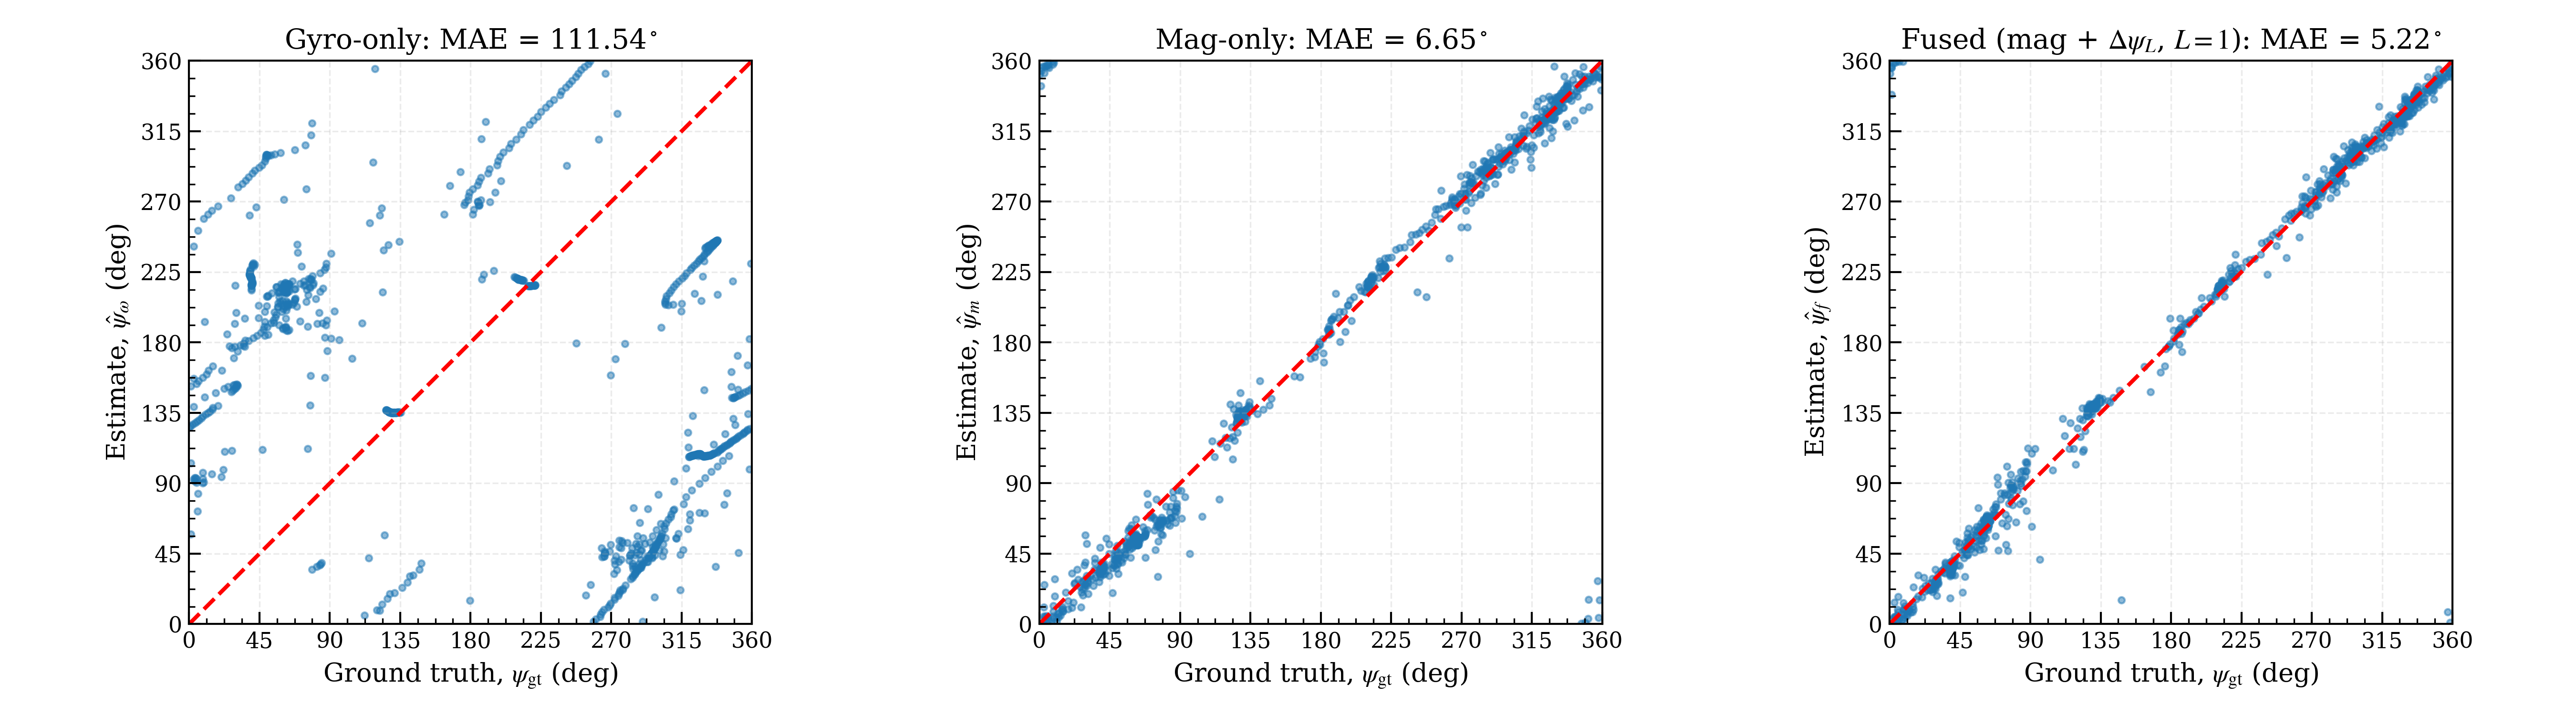
\includegraphics[width=\linewidth]{fig/psi_scatter_plots.png}
%  \caption{Scatter plots, showing the accuracy performance of the heading angle estimation from (a) Gyroscope data, (b) Magnetometer data, and (c) Fused Gyro-Magnetometer data.}
%  \label{fig:psi_scatter}
%\end{figure*}
% \begin{figure*}[!t]
%   \centering
%   % Extracted from test_compare_models_V2.py
%   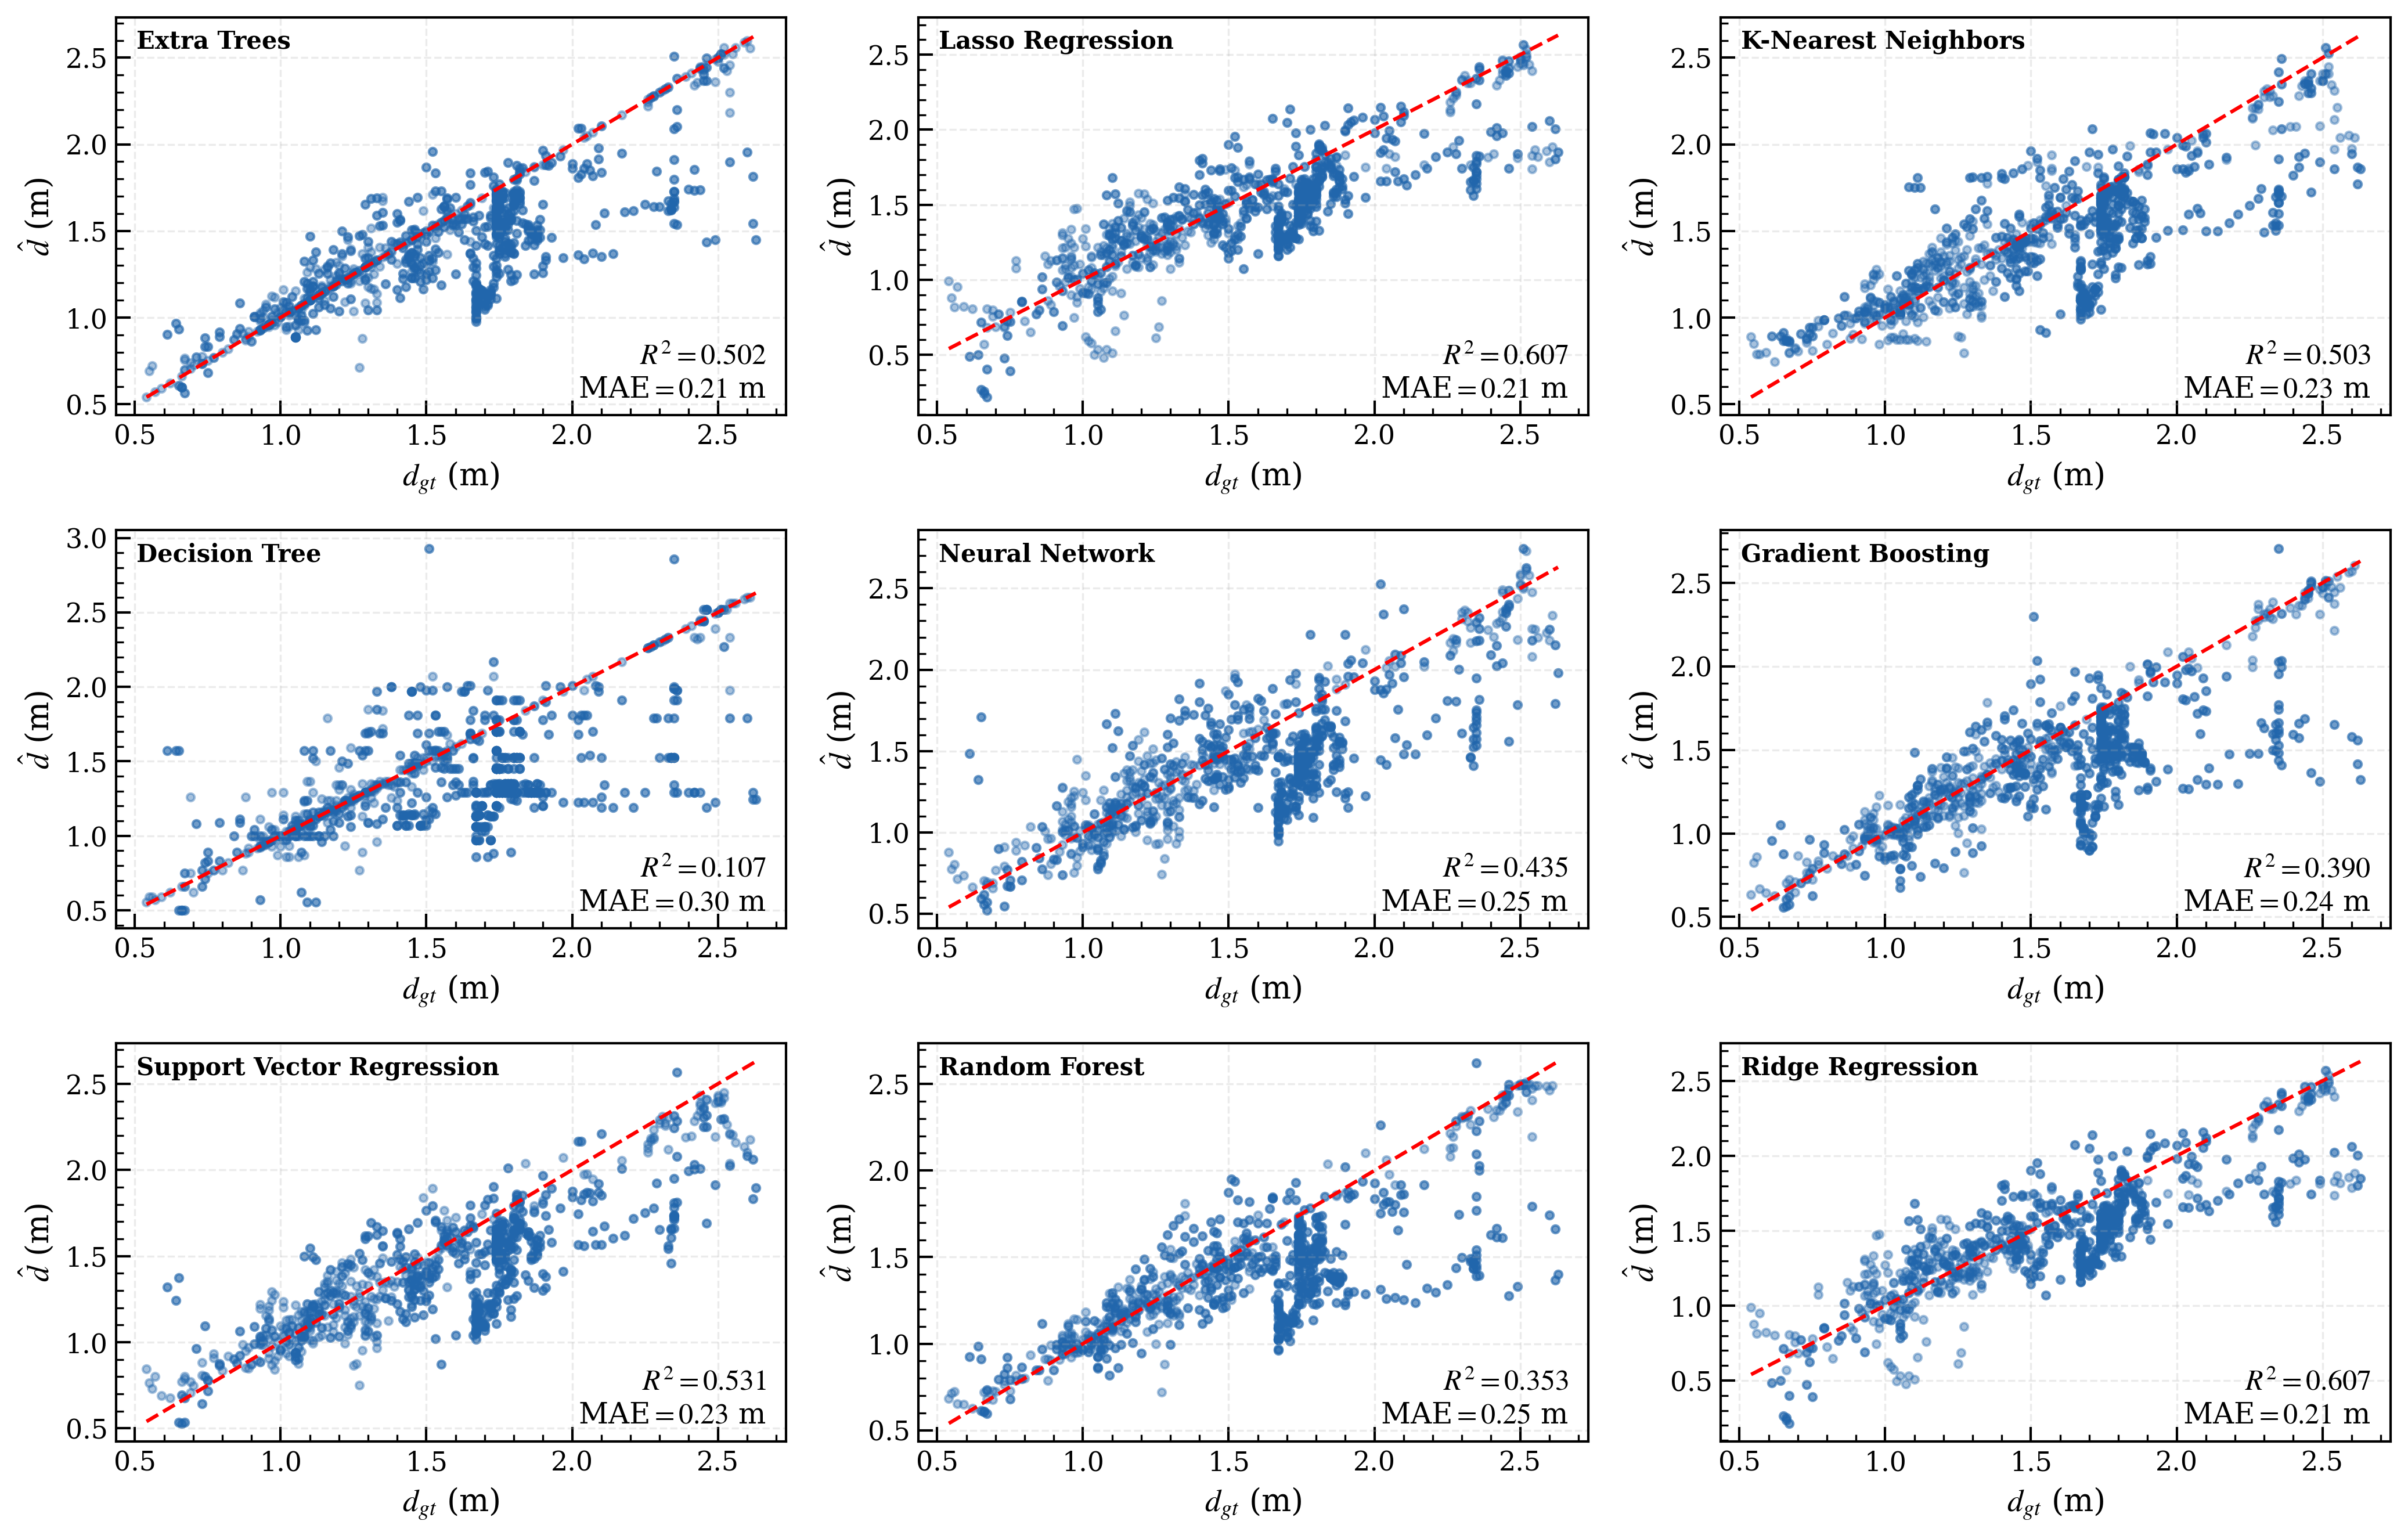
\includegraphics[width=\linewidth]{fig/distance_model_compare_indep.png}
%   \caption{Comparison of distance estimation performance when training and testing on independent datasets.}
%   \label{fig:distance_scatter}
% \end{figure*}
%\begin{figure*}[!t]
 %   \centering
 %   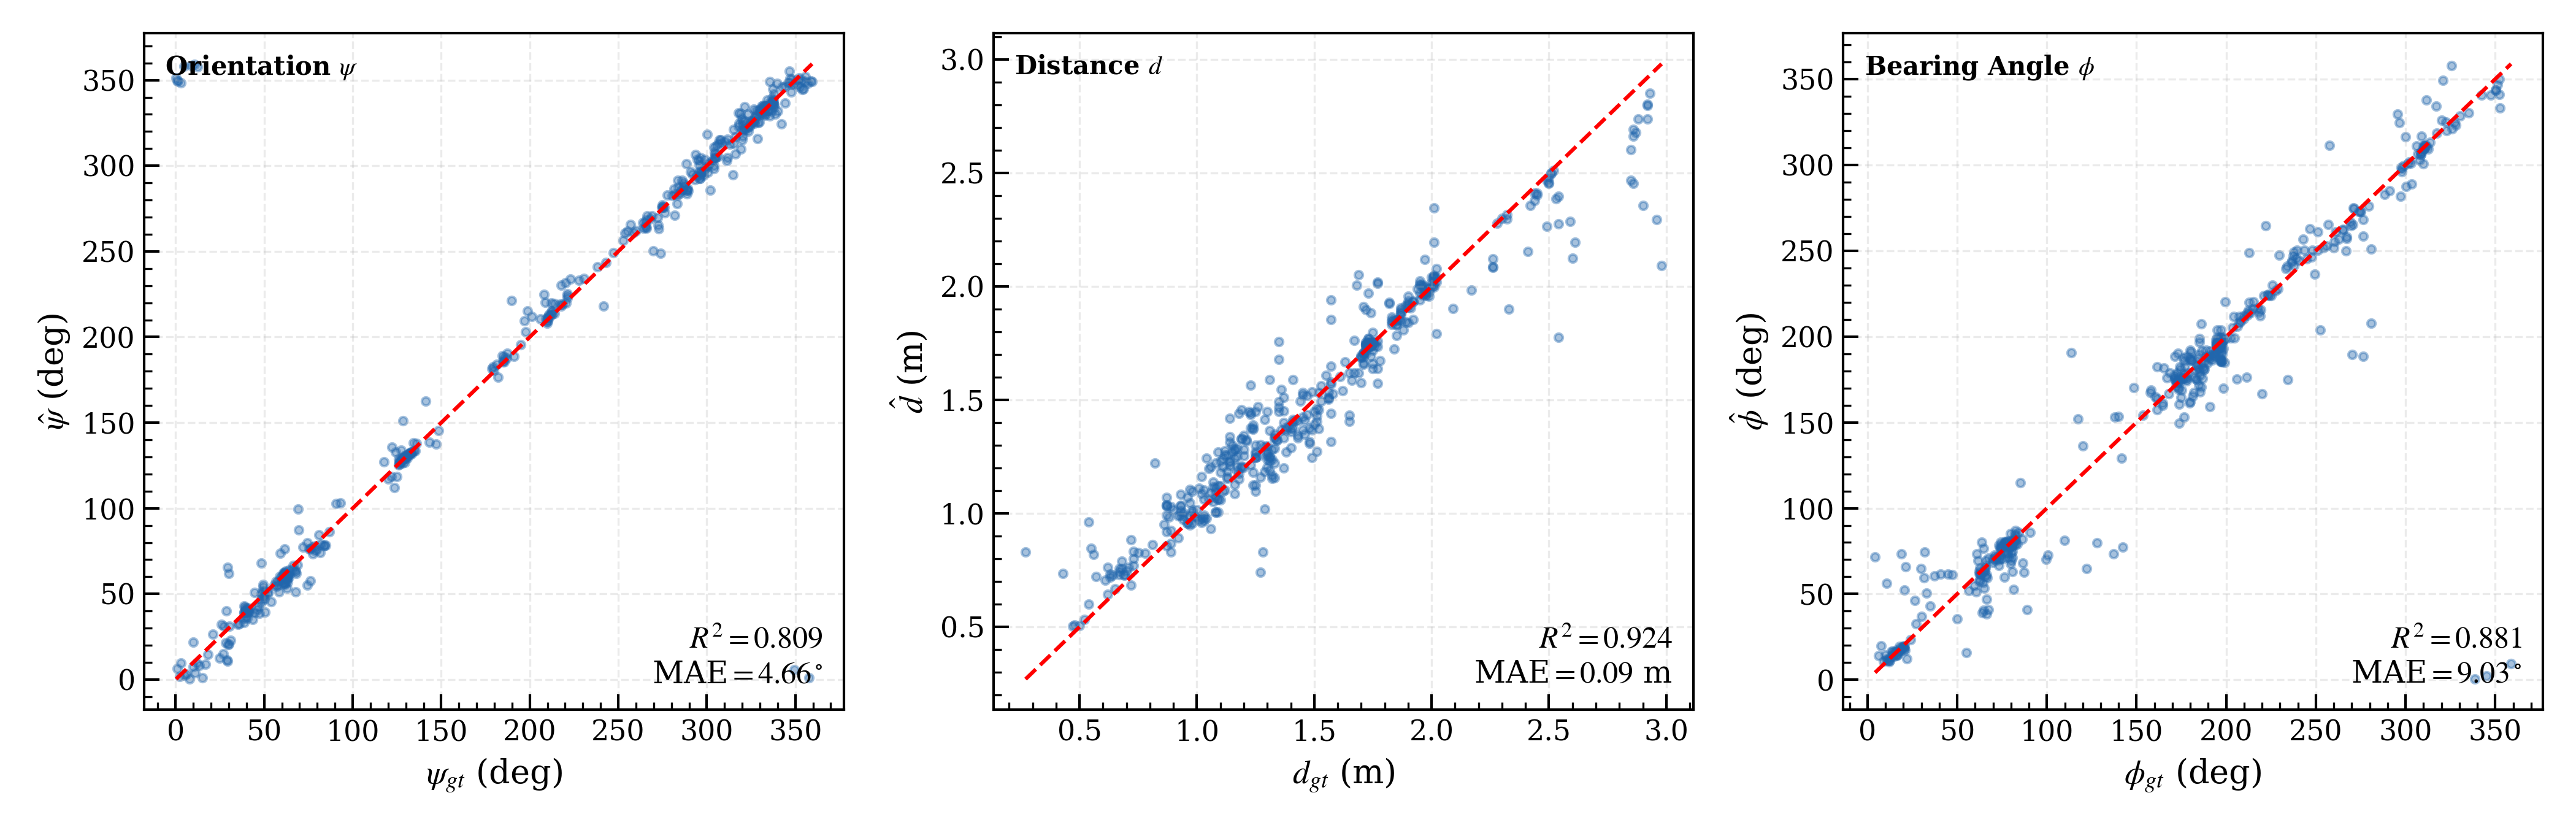
\includegraphics[width=\textwidth]{fig/combined_model_predictions.png}
%    \caption{Prediction performance of the combined Extra Trees--based estimation framework on the train--test split.}
%    \label{fig:combined_predictions}
%\end{figure*}


\begin{figure*}[!th]
  % Extracted from psi_mag_gyro_V1.py
  \centering
  \begin{subfigure}{\linewidth}
    \centering
    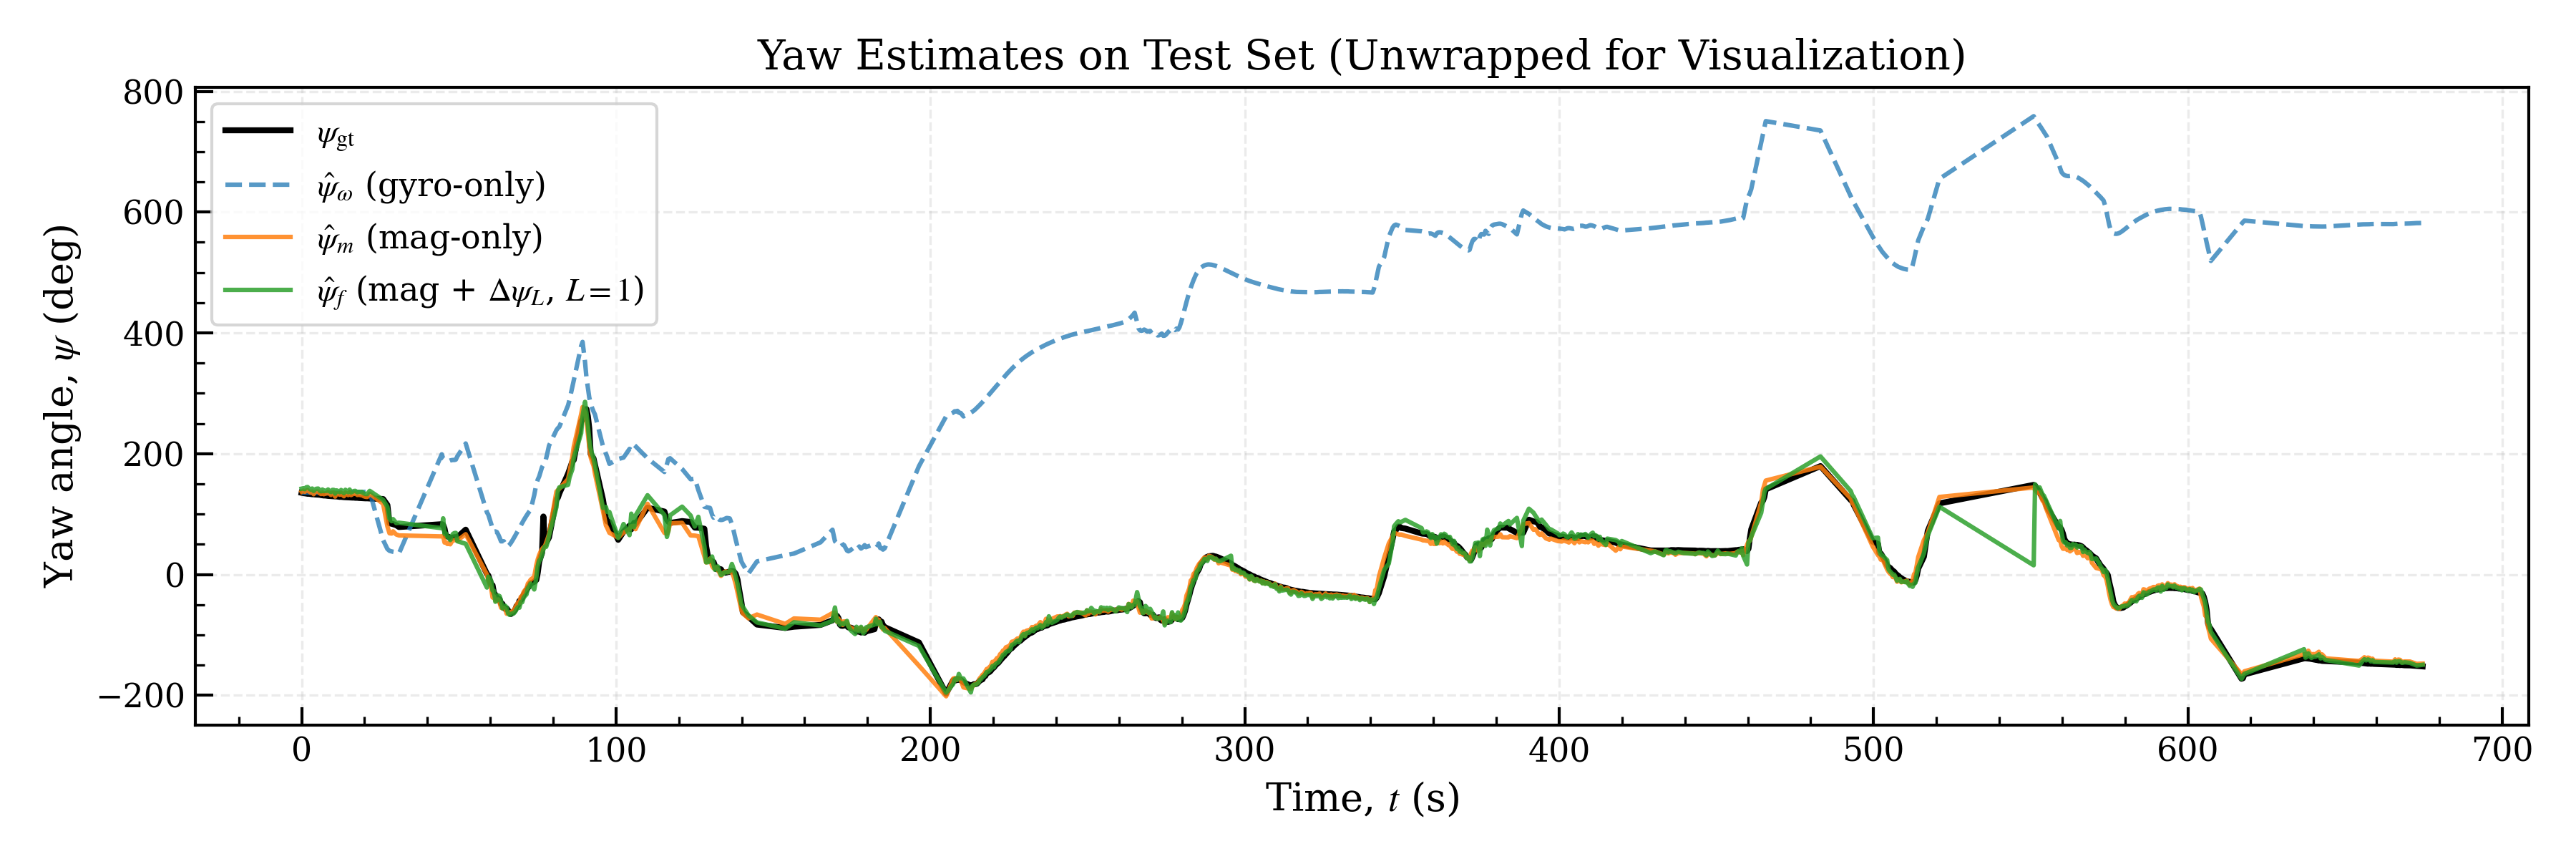
\includegraphics[width=\linewidth]{fig/psi_unwrapped_timeseries.png}
    \label{fig:psi_unwrapped}
  \end{subfigure}
  \vspace{1em}
  \begin{subfigure}{\linewidth}
    \centering
    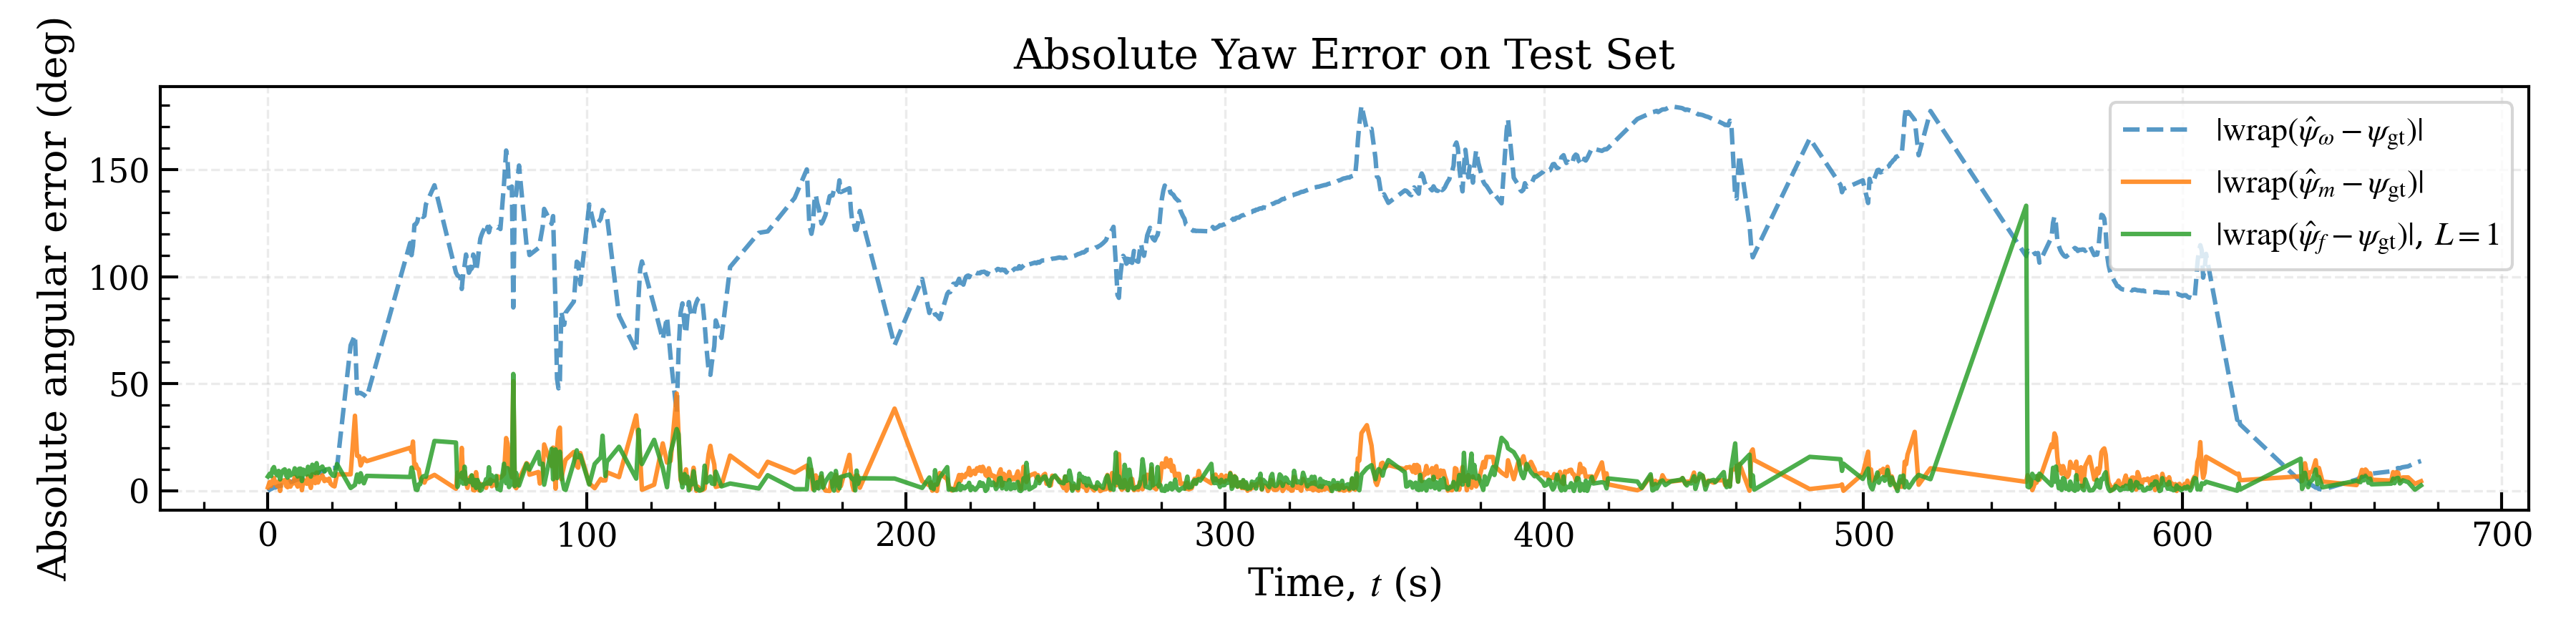
\includegraphics[width=\linewidth]{fig/psi_absolute_error_timeseries.png}
    \label{fig:psi_absolute_error}
  \end{subfigure}
  \caption{Analysis of heading angle $\psi$ estimation from IMU data: (a) unwrapped heading angle over time, and (b) absolute error compared to ground truth.}
  \label{fig:psi_timeseries}
\end{figure*}

\begin{figure}[!th]
    \centering
    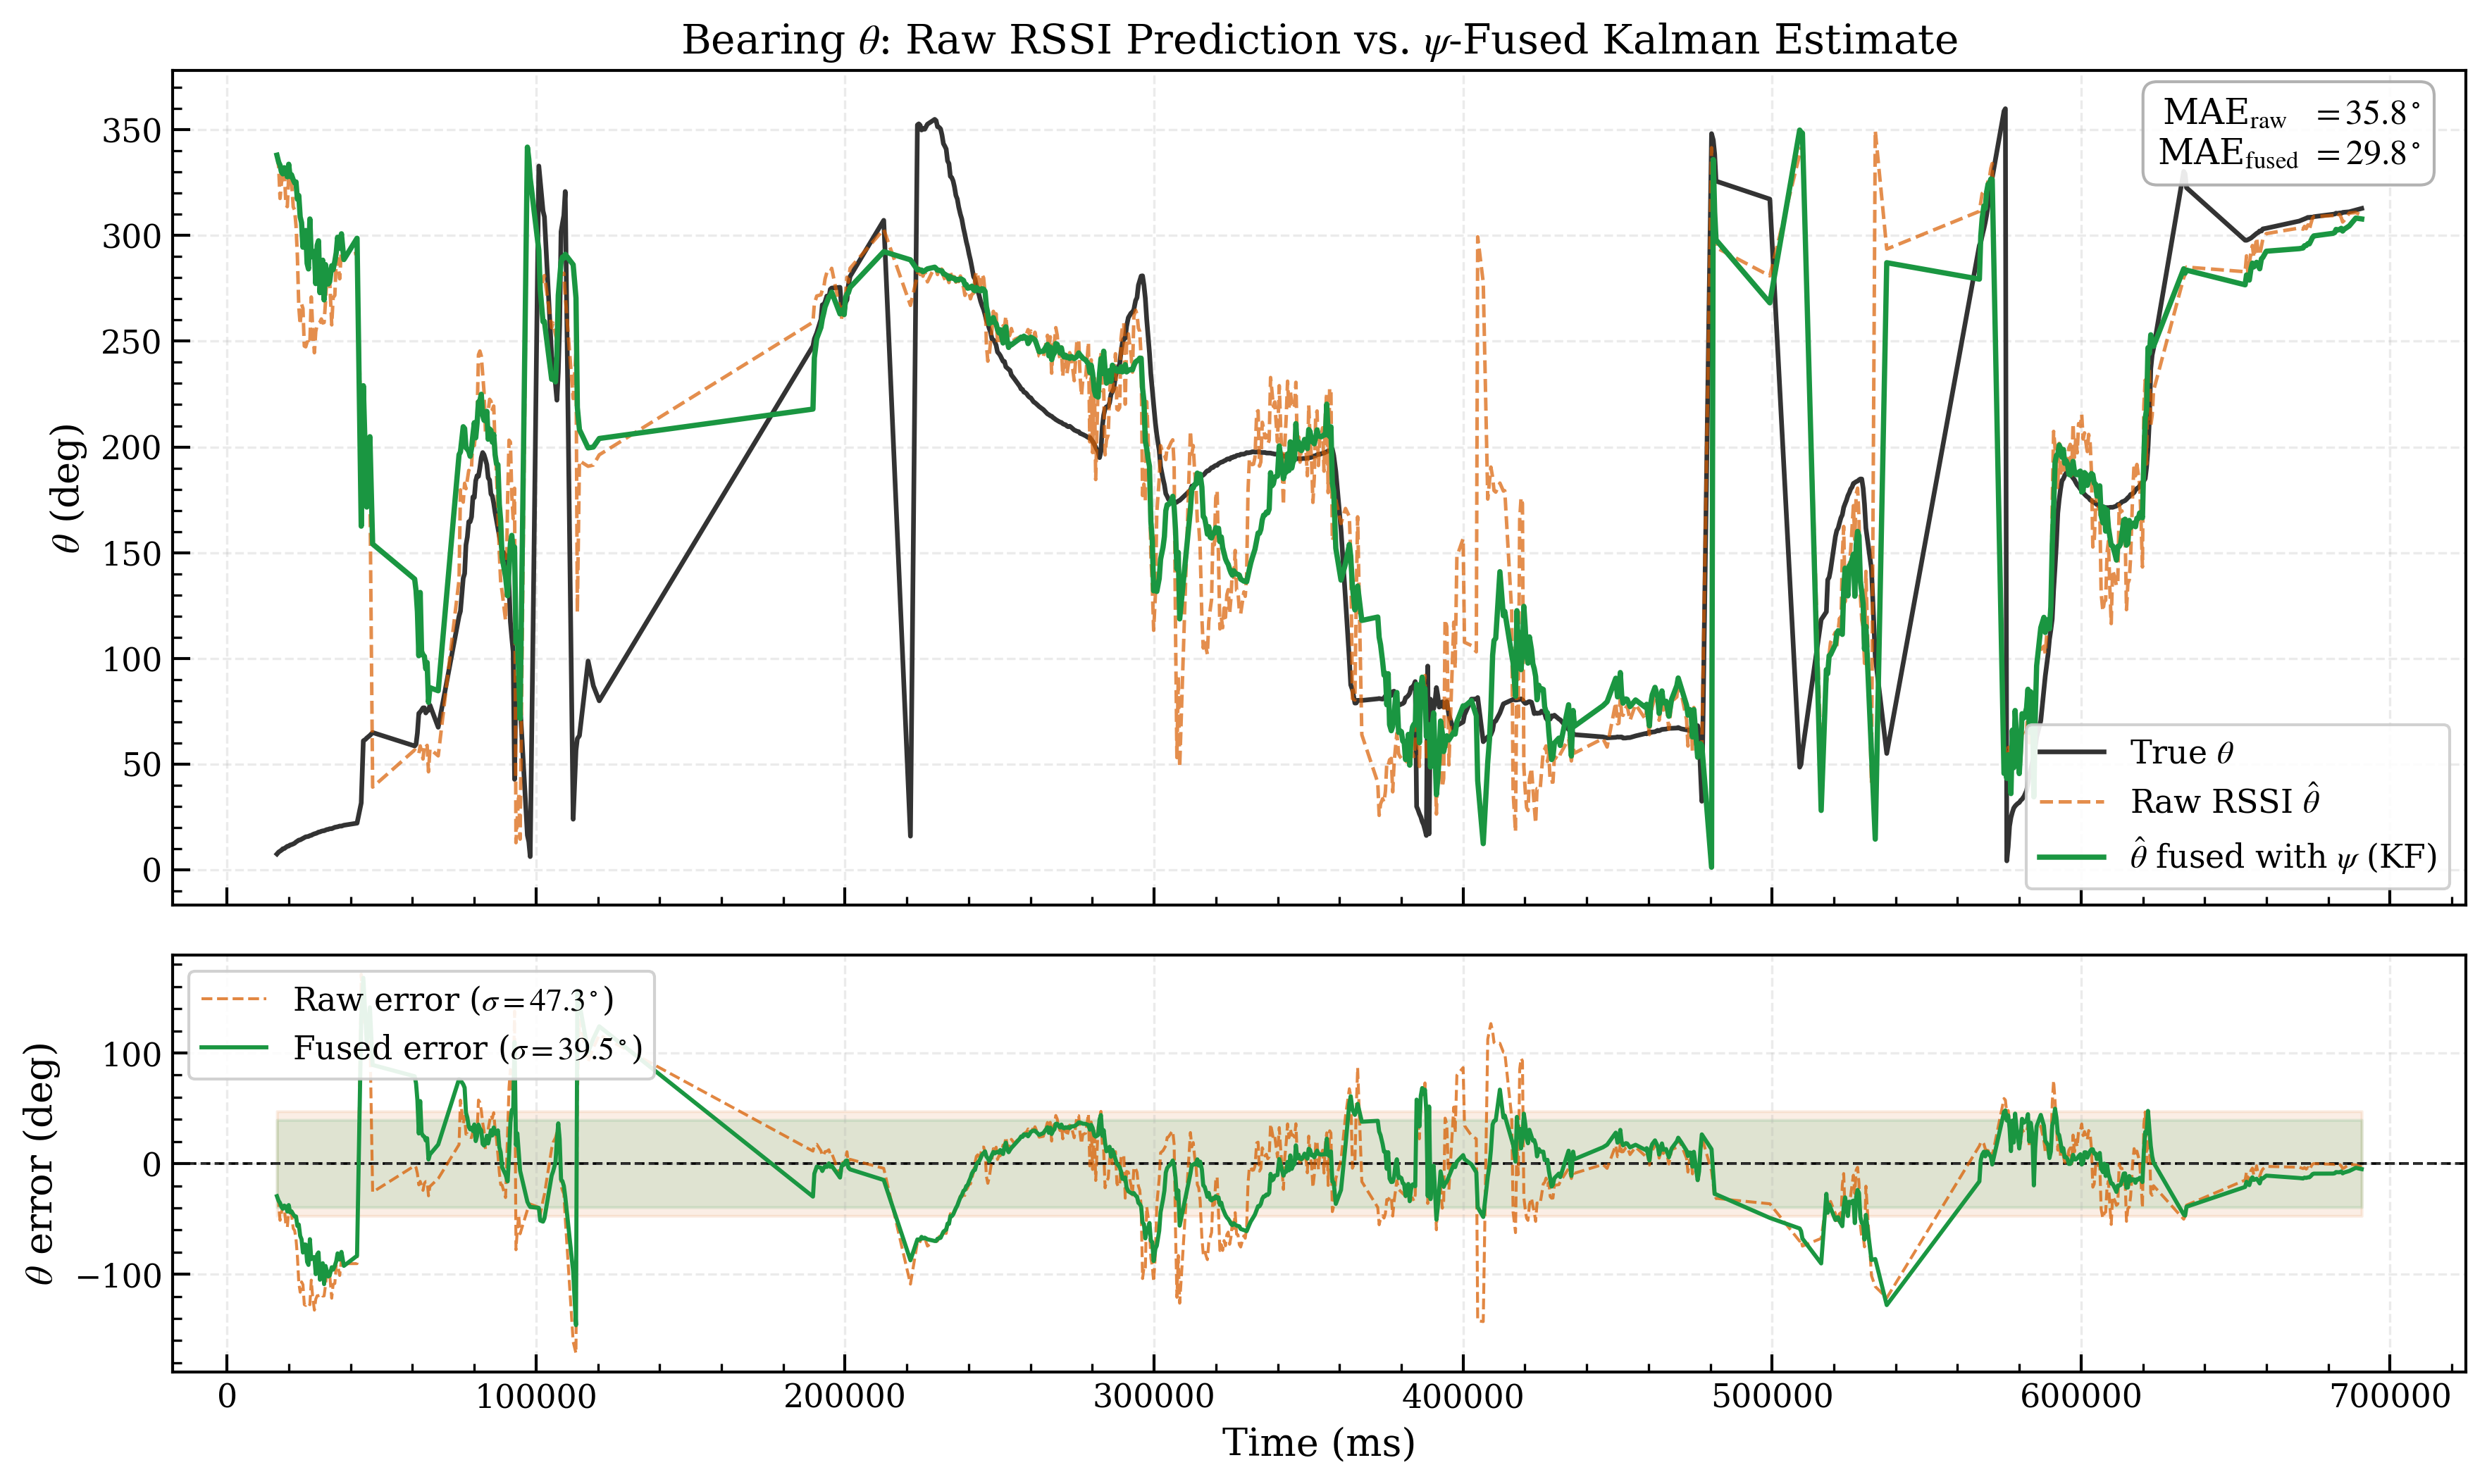
\includegraphics[width=0.48\textwidth]{fig/theta_kf_comparison.png}
    \caption{Comparison of RSSI-based bearing angle \(\theta\) estimation with and without Kalman correction.}
    \label{fig:theta_kf_comparison}
\end{figure}

\begin{figure*}[!t]
    \centering
    \begin{subfigure}[!t]{0.48\textwidth}
        \centering
        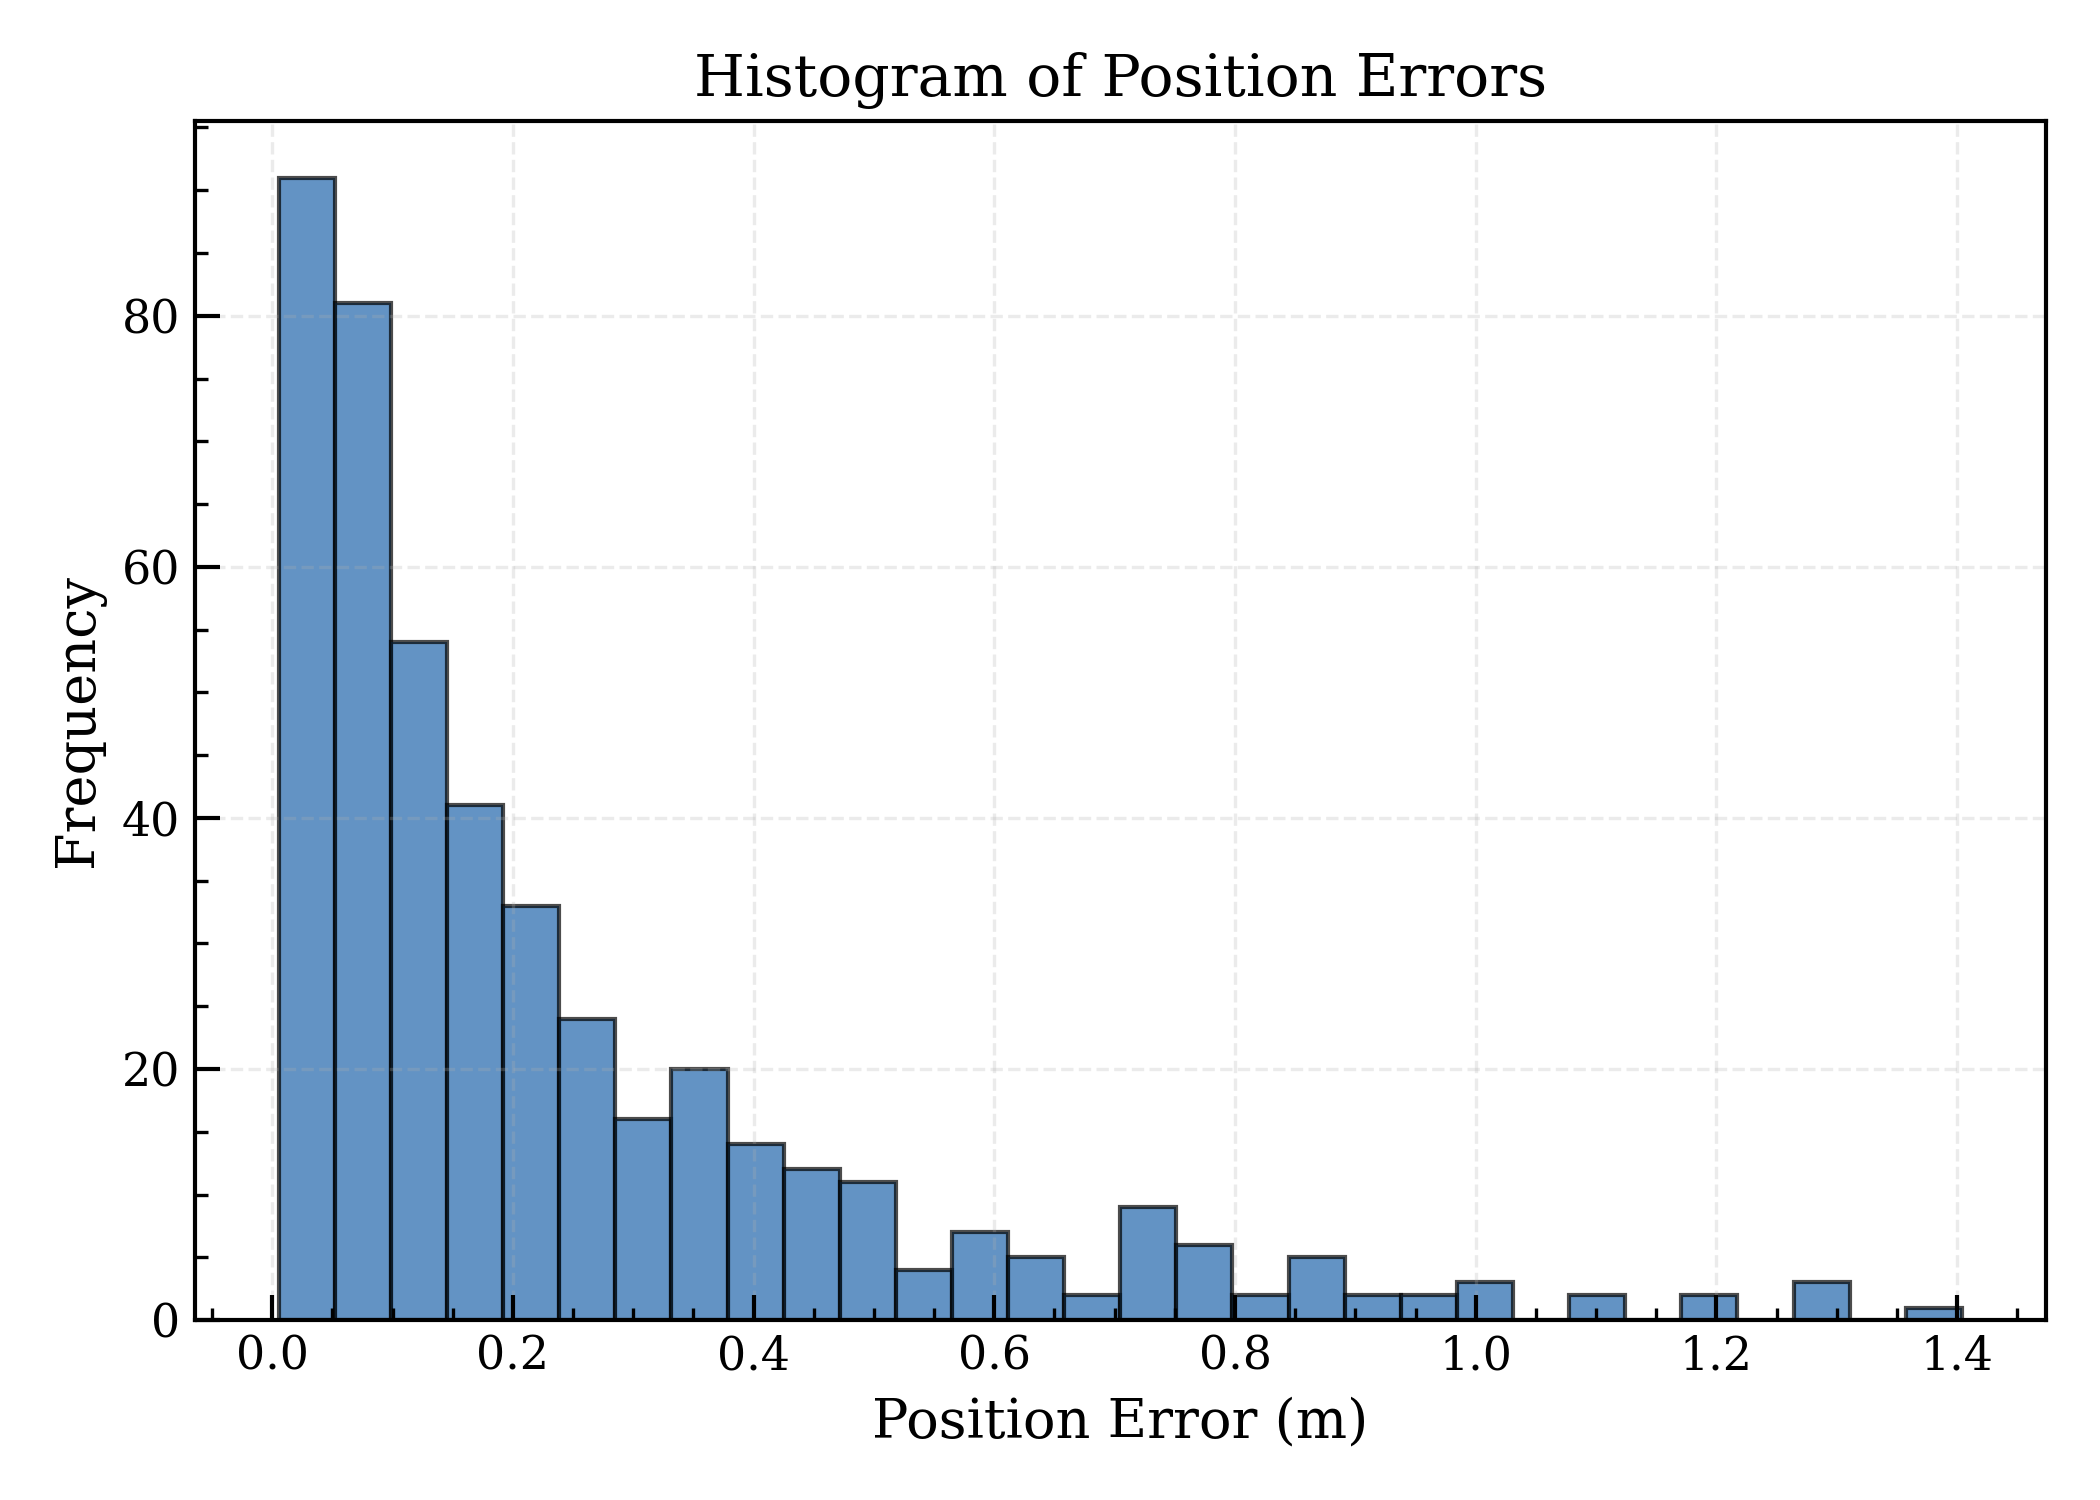
\includegraphics[width=\textwidth]{fig/position_error_histogram.png}
        \caption{Histogram of the Euclidean position error magnitude.}
        \label{fig:position_error_hist}
    \end{subfigure}
    \hfill
    \begin{subfigure}[!t]{0.48\textwidth}
        \centering
        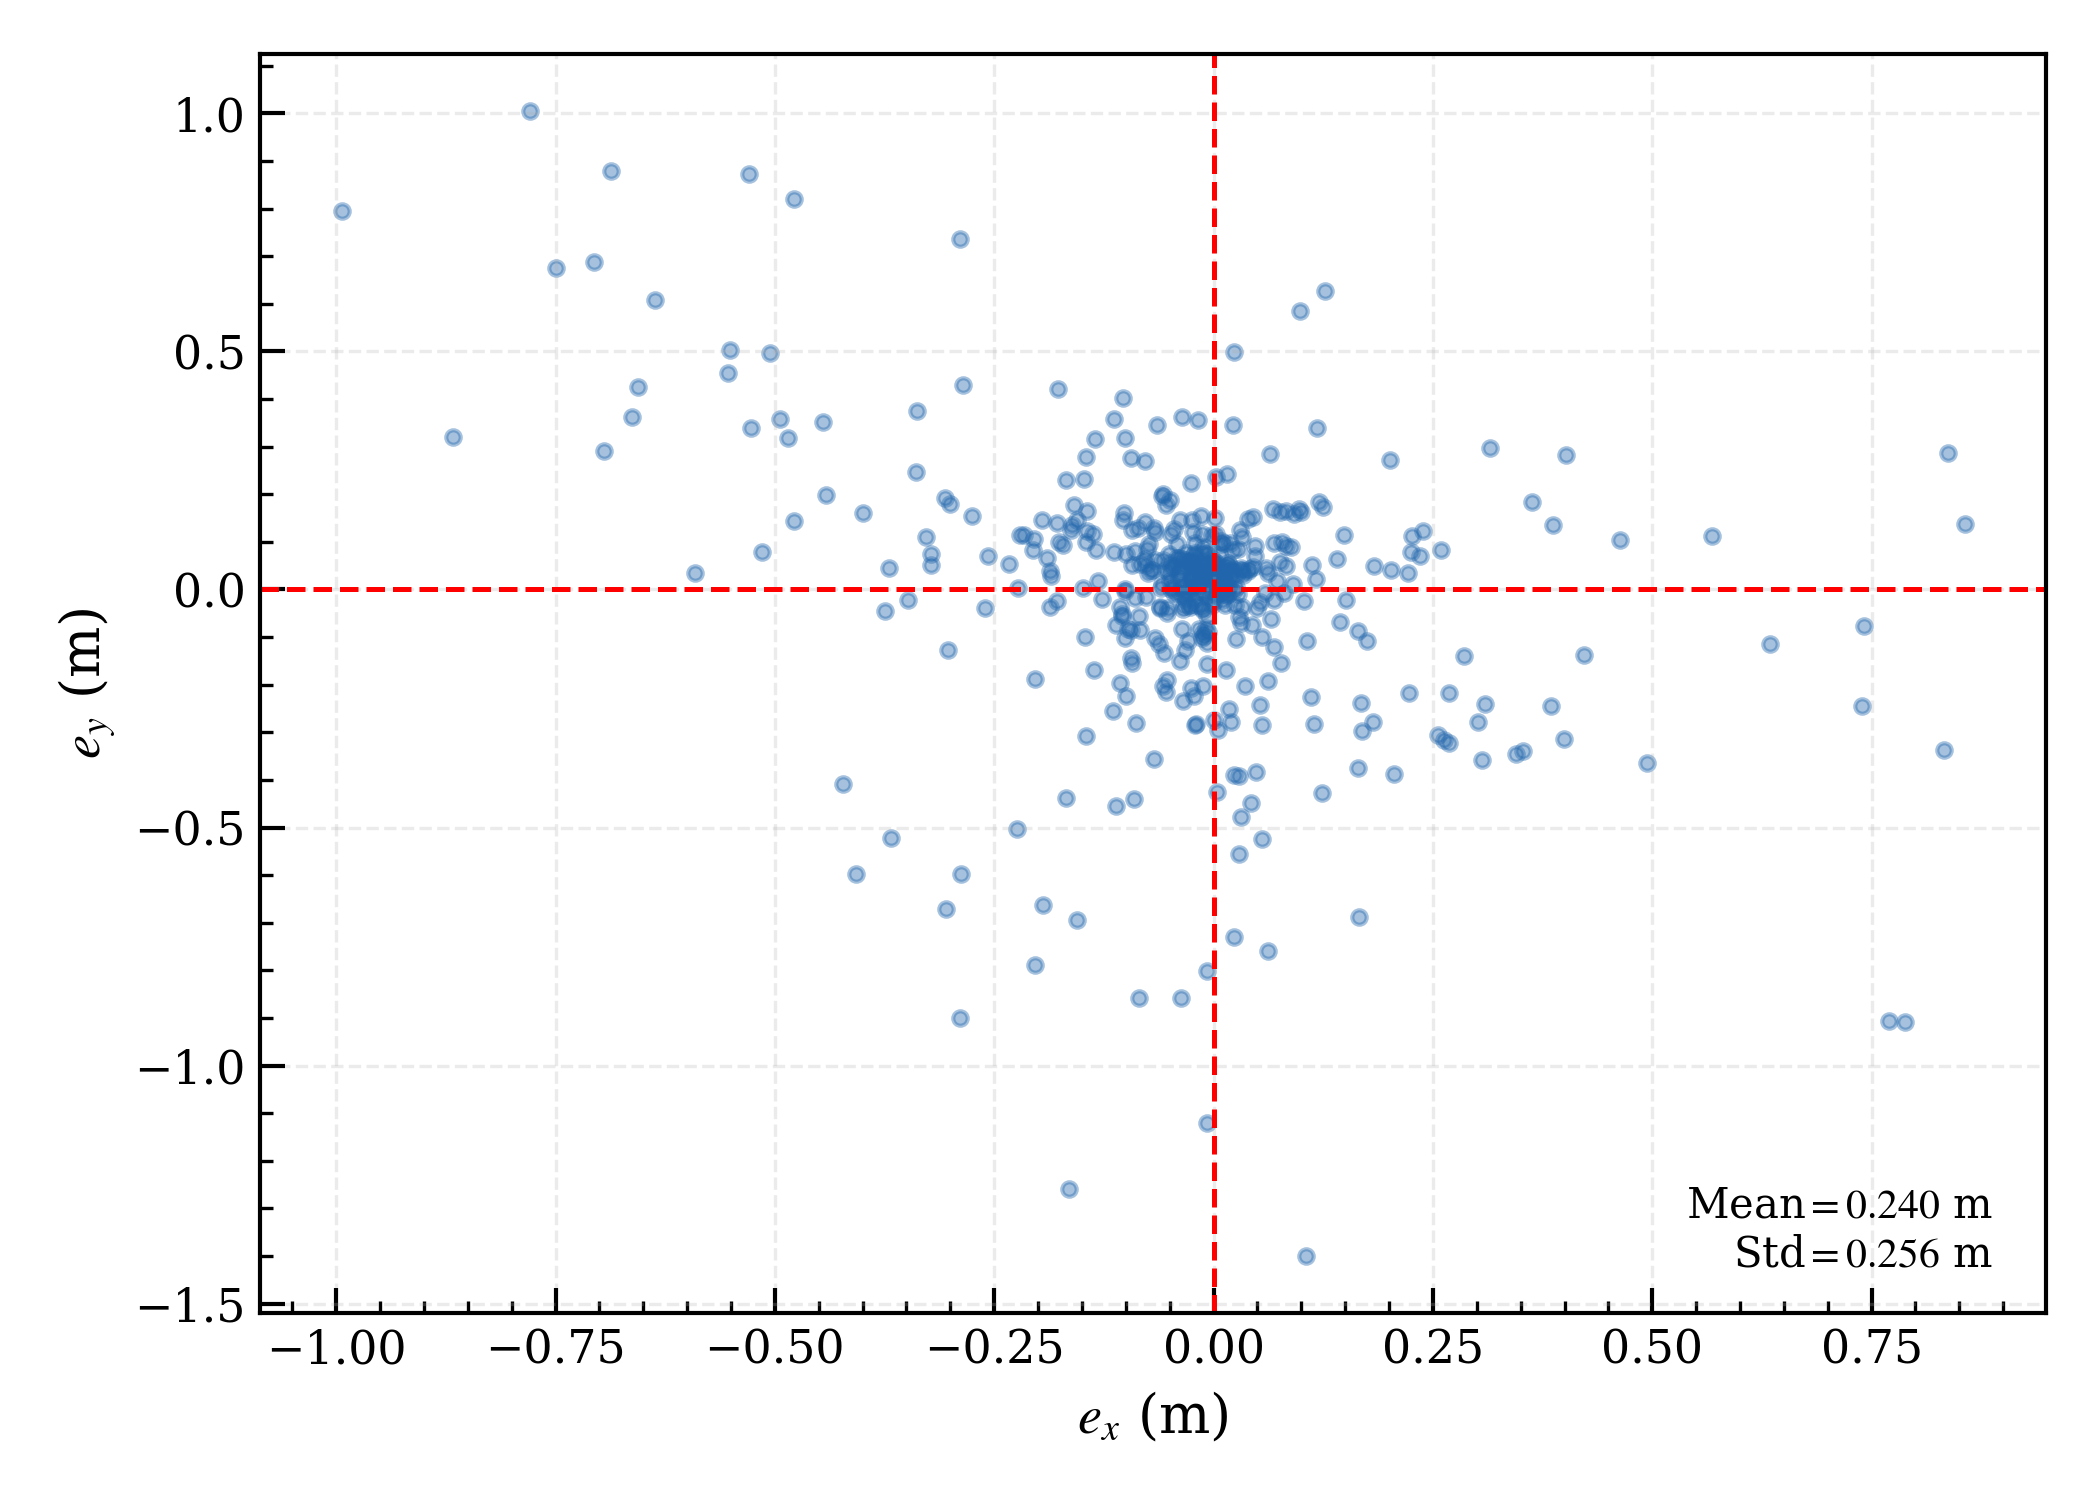
\includegraphics[width=\textwidth]{fig/position_error_scatter.png}
        \caption{Scatter plot of Cartesian position errors \((e_x,e_y)\).}
        \label{fig:position_error_scatter}
    \end{subfigure}
    \caption{Position error analysis for the combined model (train--test split).}
    \label{fig:position_error_subfigures}
\end{figure*}

\section{Results and Discussion}
Two datasets are collected: one over 0.5--3\,m range and another over 0.5--6\,m. Unless otherwise noted, models are trained on one dataset and evaluated on an independently collected one with the same antenna depth, confirming that the learned models generalize rather than overfit to a single recording. Antenna depth is controlled as it influences multipath from the water surface.
Following are the performance analysis:
\subsection{Orientation \(\psi\)}
Fig.~\ref{fig:psi_timeseries} compares the yaw estimates obtained from the gyroscope-only, magnetometer-only, and short-horizon gyro-augmented magnetometer models against the ground-truth orientation over the test sequence. For visualization purposes, the angular trajectories are shown in unwrapped form so that long-term drift and local tracking behavior can be observed continuously.

It can be seen that the gyroscope-only estimate, \(\hat{\psi}_{\omega}\), departs progressively from the ground truth as time evolves. This behavior is expected, since the gyroscope-based estimate is obtained through temporal integration of the measured angular rate, making it highly sensitive to bias and low-frequency drift. Once accumulated, this error cannot be corrected in the absence of an external absolute heading reference, which leads to the large divergence visible in the figure.

In contrast, the magnetometer-based estimate, \(\hat{\psi}_{m}\), remains closely aligned with the ground-truth yaw throughout most of the trajectory. This indicates that the planar magnetometer measurements contain sufficiently strong orientation information for direct yaw estimation, despite the presence of local distortion and measurement noise. The fused estimate, \(\hat{\psi}_{f}\), which augments the magnetometer features with a short-horizon gyroscope increment, also follows the ground-truth trajectory closely. However, its behavior is only marginally different from that of the magnetometer-only model, suggesting that under the present sampling conditions the additional gyroscope feature contributes limited improvement.

Overall, the results show that yaw is primarily observable through the magnetometer, whereas the gyroscope alone is not suitable for long-duration orientation estimation in this setup. The short-horizon fusion approach preserves stable tracking performance, but the dominant contribution to the final estimate still arises from the magnetometer-derived information.% Short term accuracy of the gyroscope can also be seen in~\ref{fig:psi_scatter} in terms of perfectly diagonally connected dots in the scatter plot. The perfectly diagonal scatter shows that gyroscope was able to capture the angular movement accurately, but the drift exist so the diagonal line is not perfectly aligned with the ground truth. 

Although Table~\ref{table:distance_orientation_model_compare} indicates that Extra Trees is the best-performing model for distance estimation under a train--test split of the same dataset, this evaluation mainly reflects interpolation within a matched measurement distribution. For shorter distance ranges, the prediction quality is even stronger.
\subsection{Bearing Angle \(\theta\)}
Fig.~\ref{fig:theta_kf_comparison} compares the raw RSSI-based bearing estimates with the corrected estimates obtained from the Kalman filter. The corrected estimates show significantly reduced noise and improved temporal consistency compared to the raw RSSI predictions, which are often scattered and erratic. This demonstrates that the Kalman correction effectively leverages the short-term rotational continuity imposed by the yaw angle to stabilize the bearing estimates, leading to more reliable position reconstruction. The results show that this method improves the overall MAE from 36 degrees to 30 degrees, which is a significant improvement for the bearing estimation task.
\subsection{Distance and Euclidean Position}
As observed in the previous comparisons, the Extra Trees regressor performs consistently well across the three estimation tasks. Therefore, in the combined analysis, the same input feature set is used to train three separate Extra Trees--based regression models for estimating \(d\), \(\theta\), and \(\psi\), respectively. For implementation convenience, these estimators are organized within a multi-output regression framework, so that training and inference can be carried out through a unified interface, while each target variable is still learned independently. To maintain consistency with the earlier evaluation, the same train--test split setting is retained here. The resulting performance indicates that the selected learning framework provides strong estimation accuracy across all three quantities. Fig.~\ref{fig:position_error_subfigures} summarizes the resulting position error distribution in terms of both magnitude and Cartesian error components.

A similar test is conducted for a another dataset which is collected in a different location and the the distance is ranged from 0.5 m to 6 m, which is more challenging than the previous dataset where the distance is ranged from 0.5 m to 3 m. It is observed that the mean absolute error in distance increases while the percentage error remains similar. The histogram in Fig.~\ref{fig:position_error_hist_6m} shows that more than 80 percent of the position estimates have an error less than 0.6 m in a range of 6 m, which is a promising result for underwater localization.
% \begin{figure*}[h]
%     \centering
%     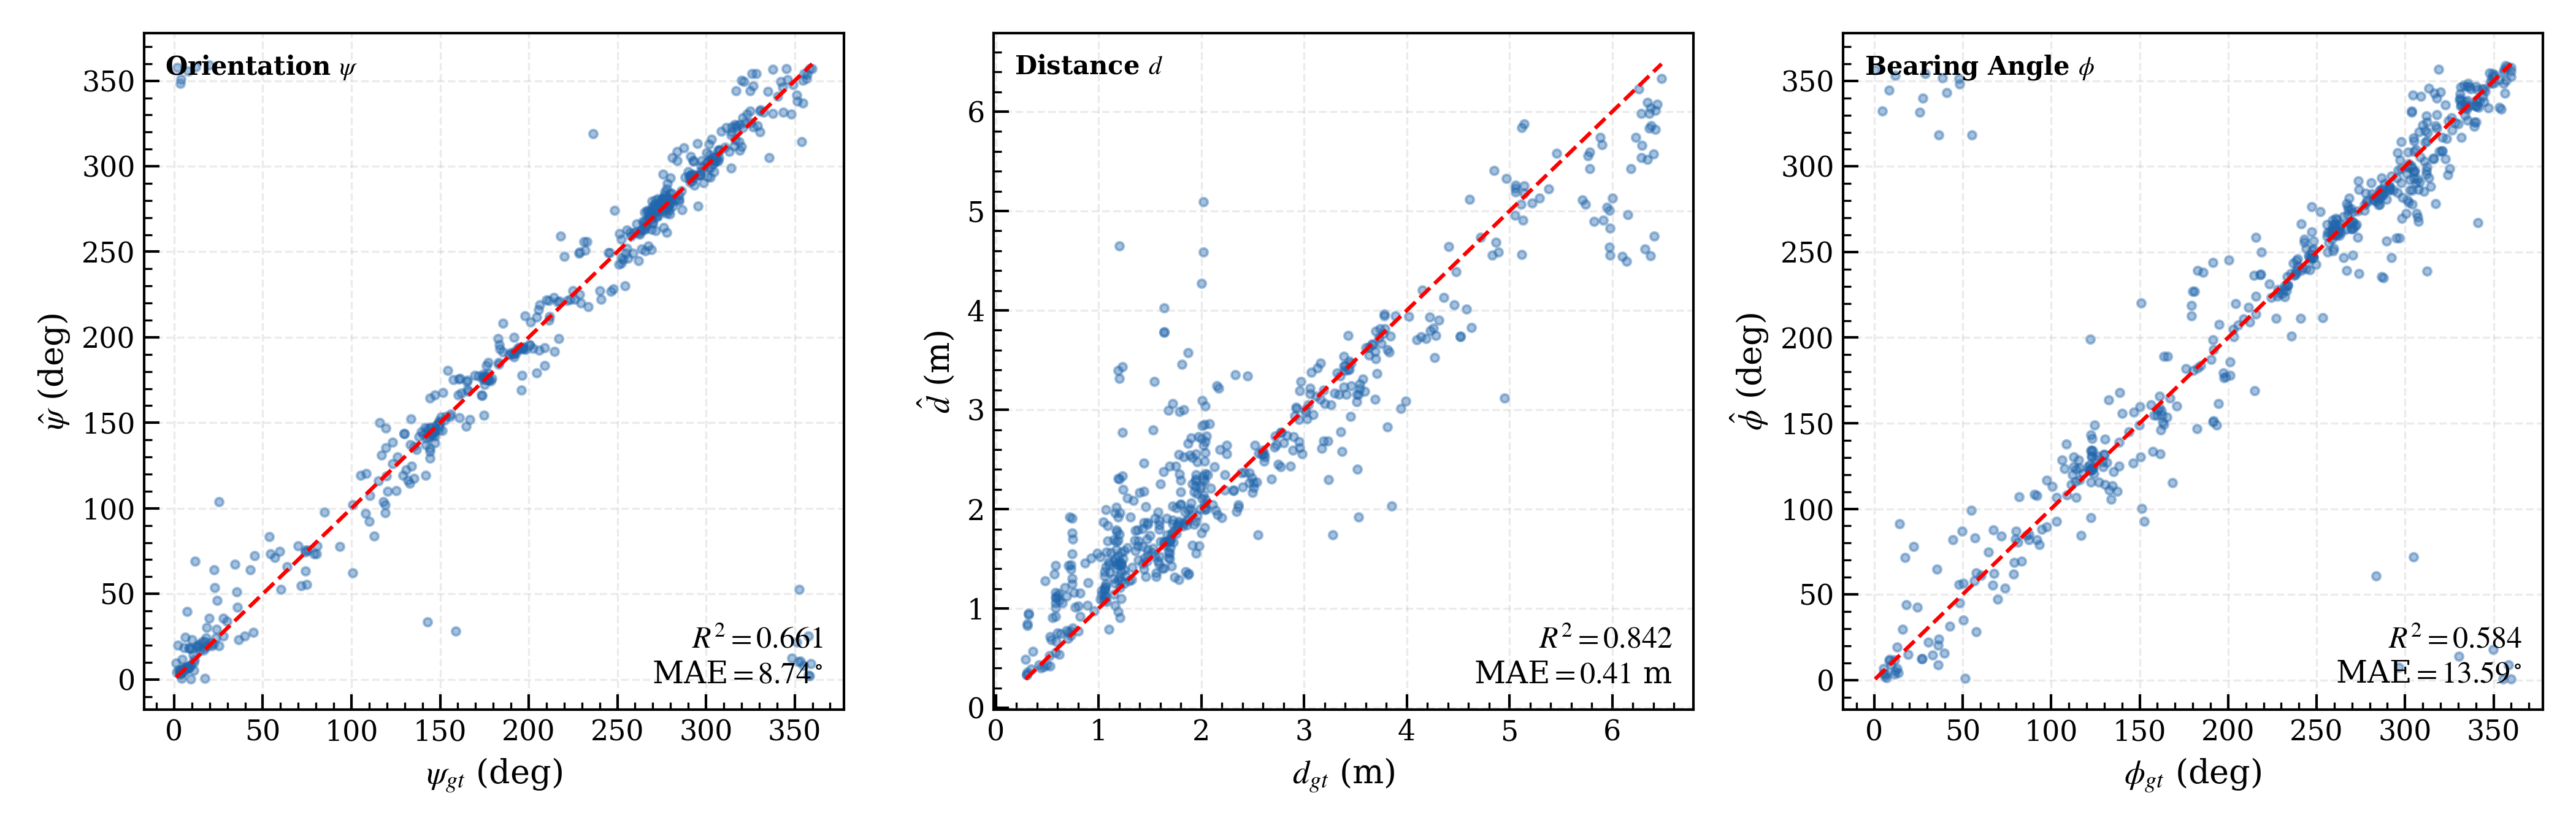
\includegraphics[width=0.48\textwidth]{fig/combined_model_predictions_6m.png}
%     \caption{Prediction performance of the combined Extra Trees--based estimation framework on the train--test split for the dataset with distance range up to 6 m.}
%     \label{fig:combined_predictions_6m}
% \end{figure*}
\begin{figure}[t]
    \centering
    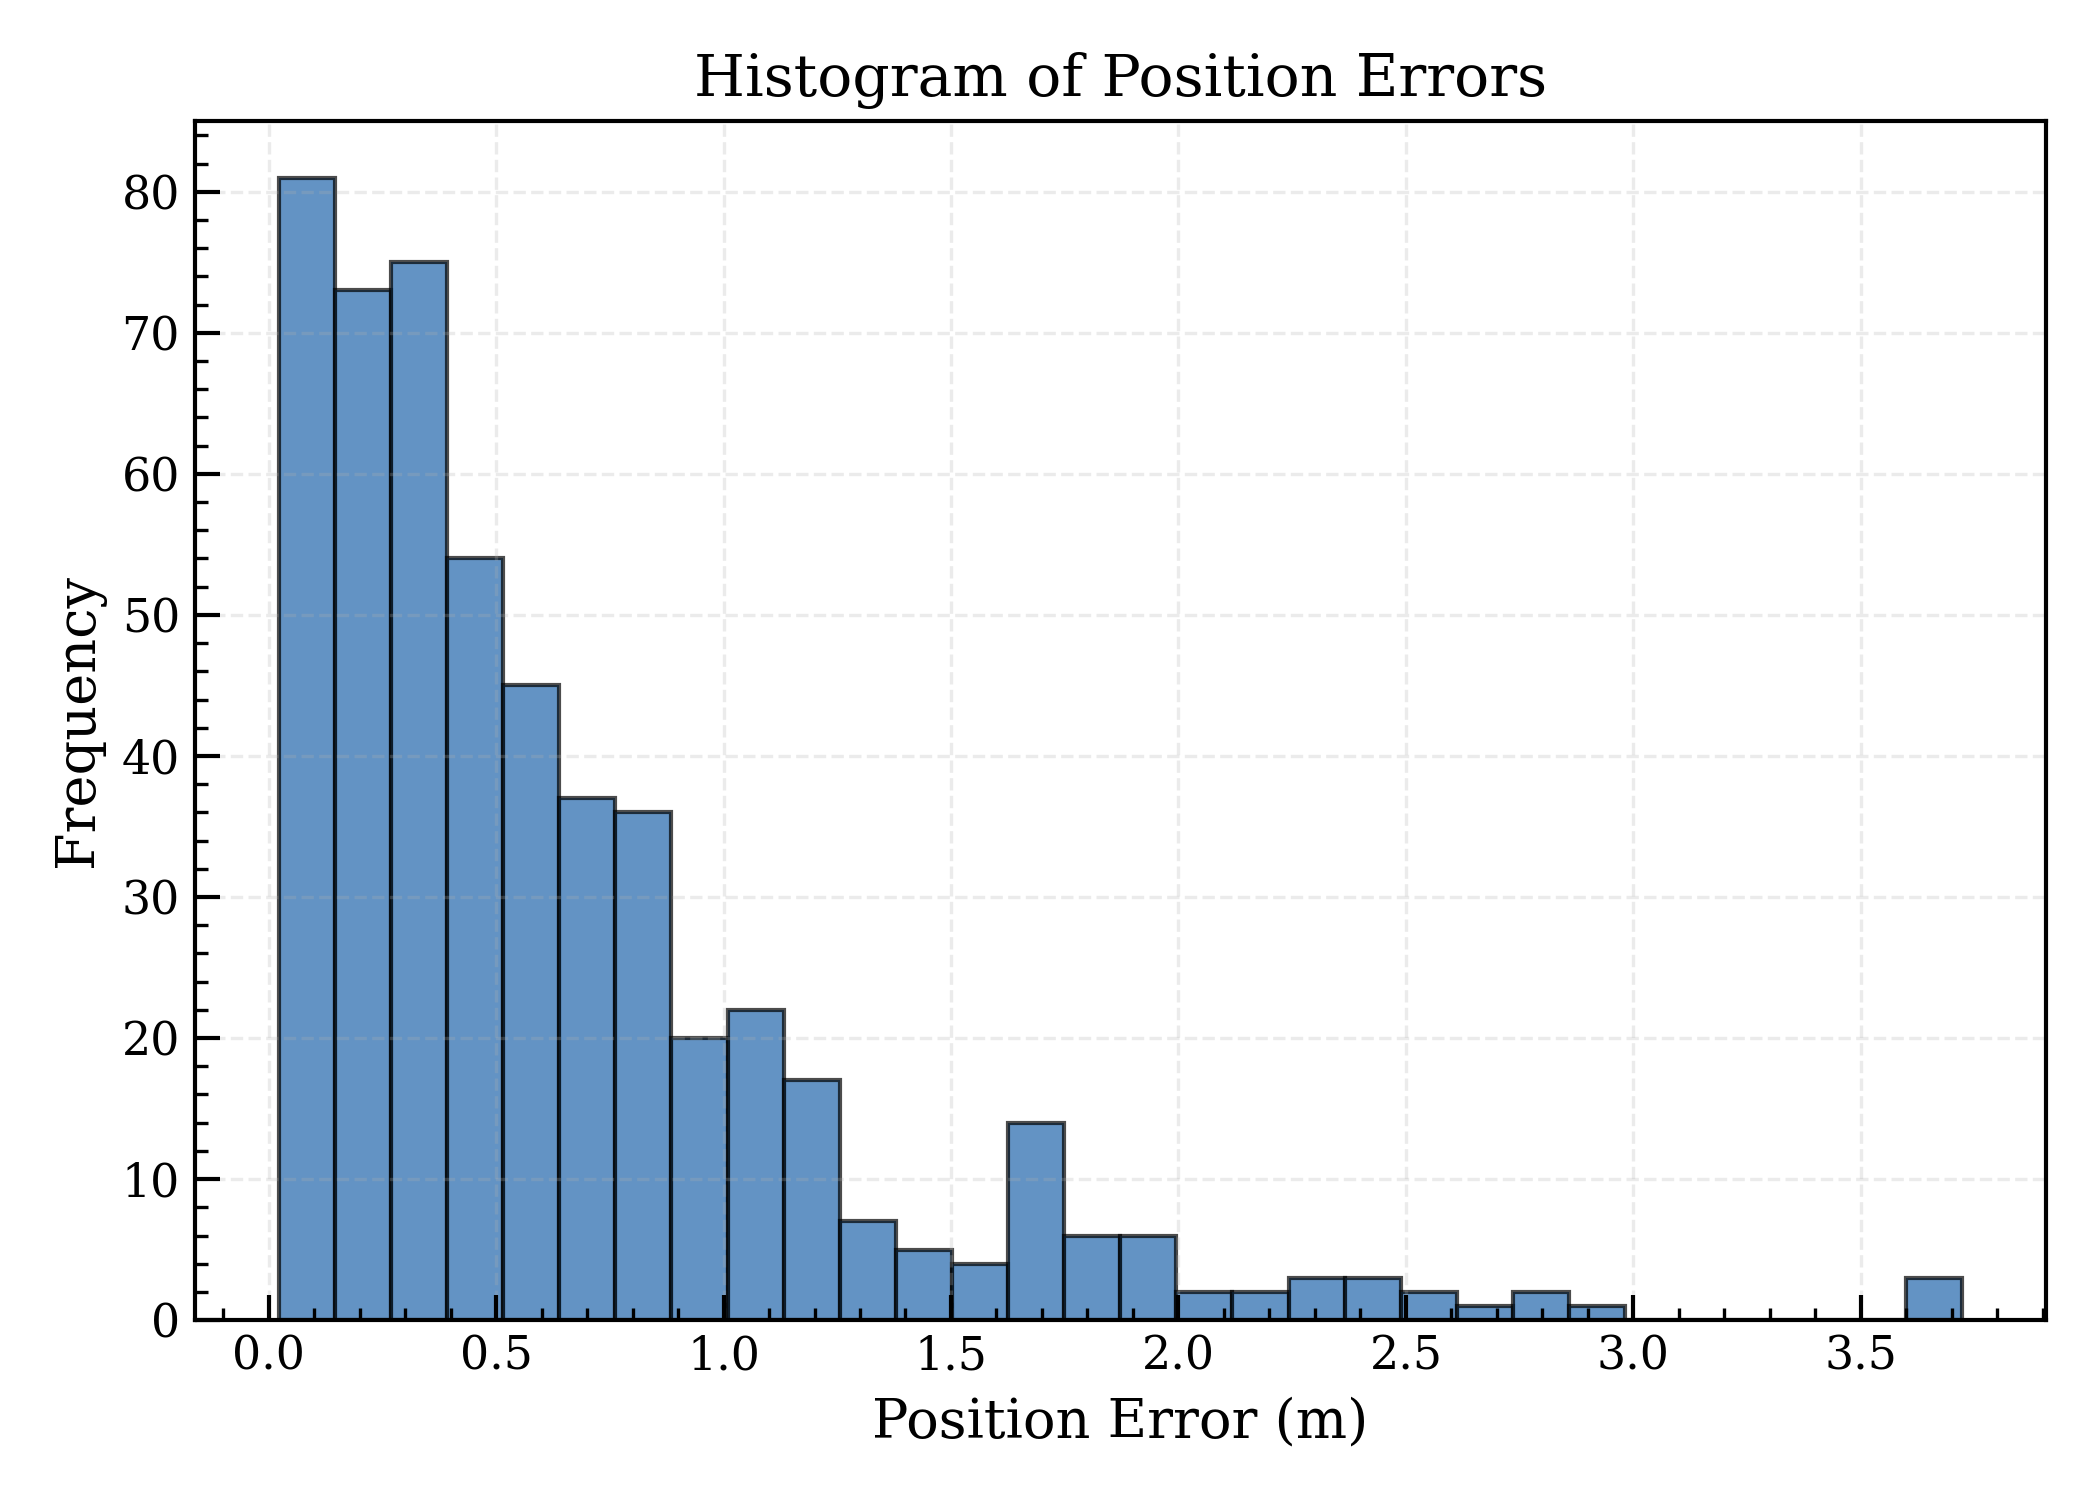
\includegraphics[width=0.48\textwidth]{fig/position_error_histogram_6m.png}
    \caption{Histogram of the Euclidean position error magnitude for the dataset with distance range up to 6 m .}
    \label{fig:position_error_hist_6m}
\end{figure}

While the presented results demonstrate that the proposed learning-based framework is capable of estimating relative position and orientation with promising accuracy, they also highlight an important practical limitation. In particular, the generalization performance across independently collected datasets is still influenced by the directional behavior of the antenna system, which remains strongly dependent on the experimental configuration. This suggests that further improvement in robustness will require not only better learning architectures and larger datasets, but also a deeper investigation of the antenna directivity itself, including its variation with installation conditions and surrounding environment. At the current stage, this should be regarded as a technological limitation of the sensing modality rather than purely a modeling limitation.

% In addition, the present study is carried out using a \(433~\mathrm{MHz}\) RF system. Future work may explore the use of lower-frequency RF bands as an alternative sensing modality, since they may offer different propagation characteristics and potentially improved operating range depending on the medium and system design. Such extensions would require dedicated experimental validation, but they open an interesting direction for broadening the applicability of the proposed framework beyond the specific hardware configuration considered in this work.

\section{Conclusion}
This paper presents a physics-aware learning framework for application in short-range underwater relative localization using Sub-GHz RF RSSI measurements. The proposed approach fuses magnetometer and short-horizon gyroscope features to estimate the receiver heading, while realizing the clues from the multi-antenna RSSI measurements and relative position, based on a learning-based model without relying only on simplified analytical path-loss or ideal antenna models. The experimental results demonstrate that the proposed framework can estimate relative range, bearing, and position in a fresh water, while the RSSI analysis shows that practical effects such as directional gain variation, enclosure and mounting effects, and multipath distortions strongly influence the measured signal strength. These observations motivate the use of a data-driven framework that can implicitly account for complex hardware and environmental effects.

This paper presents a physics-aware learning framework for application in short-range underwater relative localization using Sub-GHz RF RSSI measurements. The proposed approach fuses magnetometer and short-horizon gyroscope features to estimate the receiver heading, while realizing the clues from the multi-antenna RSSI measurements and relative position, based on a learning-based model without relying only on simplified analytical path-loss or ideal antenna models. The experimental results demonstrate that the proposed framework can estimate relative range, bearing, and position in a fresh water, while the RSSI analysis shows that practical effects such as directional gain variation, enclosure and mounting effects, and multipath distortions strongly influence the measured signal strength. These observations motivate the use of a data-driven framework that can implicitly account for complex hardware and environmental effects.

\section*{Acknowledgment}
The authors would like to thank the members of the Bio-Inspired Robotics Lab at University of Houston, and support staff at the Department of Mechanical and Aerospace Engineering for their assistance. This research was sponsored by the Ocean Energy Safety Institute Consortium (OESIC) through a grant from the U.S. Department of the Interior, Bureau of Safety and Environmental Enforcement (BSEE), and the U.S. Department of Energy (DOE) and was accomplished under Agreement Number E21AC00000. The views and conclusions contained in this document are those of the authors and should not be interpreted as representing the opinions or policies of the U.S. Government. Mention of trade names or commercial products does not constitute their endorsement by the U.S. Government.

\begin{nomenclature}
\EntryHeading{Geometry and Estimated States}
\entry{$(x_t,y_t)$}{Transmitting-agent position in the world frame}
\entry{$(x_r,y_r)$}{Receiving-agent position in the world frame}
\entry{$\mathbf{p}_{\mathrm{gt},k}$}{Ground-truth receiver position from the overhead vision system}
\entry{$\hat{x}_k,\hat{y}_k$}{Estimated absolute receiver position components}
\entry{$\hat{x}_{\mathrm{rel},k},\hat{y}_{\mathrm{rel},k}$}{Estimated receiver position components in the transmitter frame}
\entry{$d_{\mathrm{gt},k}$}{Ground-truth transmitter--receiver distance}
\entry{$\hat{d}_k$}{Estimated transmitter--receiver distance}
\entry{$\theta_{\mathrm{gt},k}$}{Ground-truth relative bearing in the receiver body frame}
\entry{$\hat{\theta}_k$}{Estimated relative bearing}
\entry{$\psi_{\mathrm{gt},k}$}{Ground-truth yaw angle in the world frame}
\entry{$\hat{\psi}_k$}{Estimated yaw angle in the world frame}

\EntryHeading{Sensor Measurements and Features}
\entry{$\mathbf{S}_k$}{Synchronized RSSI vector, $[S_{1,k},S_{2,k},S_{3,k},S_{4,k}]^T$}
\entry{$S_{r,i}$}{RSSI measured at receiving antenna $i$}
\entry{$\Delta S$}{RSSI difference between adjacent antennas}
\entry{$\mathbf{m}_k$}{Planar magnetometer measurement, $[m_{x,k},m_{y,k}]^T$}
\entry{$\omega_k$}{Measured gyroscope yaw rate at sample $k$}
\entry{$b_g$}{Gyroscope bias}
\entry{$\Delta t_k$}{Sampling interval at sample $k$}
\entry{$\delta\psi_k$}{Incremental yaw change from gyroscope at sample $k$}
\entry{$\Delta\psi_k^{(L)}$}{Short-horizon accumulated yaw increment over window length $L$}
\entry{$\mathbf{a}_k$}{Three-axis accelerometer measurement at sample $k$}
\entry{$t_k$}{Localization-device timestamp}
\entry{$t_k^{\mathrm{comp}}$}{Host-computer timestamp for synchronization}

\EntryHeading{Learning and Kalman Correction}
\entry{$\mathbf{x}_k^{(m)}$}{Magnetometer feature vector}
\entry{$\mathbf{x}_k^{(g)}$}{Short-horizon gyroscope feature vector}
\entry{$\mathbf{x}_k^{(f)}$}{Fused magnetometer--gyroscope feature vector}
\entry{$\mathbf{x}_k^{(d)}$}{Distance/combined model input feature vector}
\entry{$\mathbf{y}_k$}{Cosine--sine target representation for angular regression}
\entry{$\hat{\mathbf{y}}_k^{(m)}$}{Predicted cosine--sine output of the magnetometer model}
\entry{$f_m(\cdot),f_d(\cdot)$}{Learned nonlinear regression mappings}
\entry{$\Theta_m,\Theta_d$}{Trainable parameters of the magnetometer and distance/combined models}
\entry{$\hat{\theta}_k^{(\mathrm{RSSI})}$}{Raw RSSI-based bearing estimate}
\entry{$\hat{\theta}_k^{-}$}{Predicted bearing before Kalman measurement update}
\entry{$\hat{\theta}_k^{+}$}{Kalman-corrected bearing estimate}
\entry{$z_k$}{Kalman measurement from the RSSI-based bearing model}
\entry{$K_k$}{Kalman gain}
\entry{$P_k$}{Kalman error covariance}

\EntryHeading{RF Propagation and Hardware Parameters}
\entry{$P_t$}{Transmitted RF power}
\entry{$P_r$}{Received RF power}
\entry{$G_t$}{Transmitter antenna gain}
\entry{$G_r(\theta)$}{Receiver antenna gain as a function of arrival angle}
\entry{$G_{\max}$}{Maximum receiver antenna gain at boresight}
\entry{$L(d)$}{Path loss as a function of propagation distance}
\entry{$\alpha_\omega$}{Medium attenuation coefficient}
\entry{$\alpha_b$}{Antenna half-power beamwidth}
\entry{$\lambda$}{RF wavelength}
\entry{$f_c$}{Carrier frequency}
\entry{$f_{rf}$}{RF carrier frequency used in the analytical attenuation model}
\entry{$R_b$}{Nominal RF data rate}
\entry{$S_{\min}$}{Nominal receiver sensitivity}
\entry{$T_{\mathrm{air}}$}{Packet airtime}
\entry{$r_{\mathrm{comm}}$}{Maximum tested reception distance}
\entry{$r_{\mathrm{loc}}$}{Evaluated localization range}
\entry{$\sigma$}{Water conductivity}
\entry{$\theta_i$}{Boresight direction of antenna $i$}
\entry{$\theta_{\mathrm{rel}}$}{Bearing offset relative to the selected antenna boresight}
\entry{$\theta_{\mathrm{AoA}}$}{Analytical angle-of-arrival estimate}
\entry{$d_{\mathrm{RSS}}$}{Analytical RSSI-based distance estimate}
\entry{$N$}{Number of receiving antennas}

\EntryHeading{Subscripts and Superscripts}
\entry{$t$}{Transmitting agent or transmitter-related quantity}
\entry{$r$}{Receiving agent or receiver-related quantity}
\entry{$k$}{Sample index}
\entry{$\mathrm{gt}$}{Ground-truth quantity from the overhead vision system}
\entry{$\mathrm{rel}$}{Quantity expressed in the transmitter-relative frame}
\entry{$xy$}{Planar $x$-$y$ components}
\entry{$\mathrm{rf}$}{RF-related quantity}
\entry{$m,g,f,d$}{Magnetometer, gyroscope, fused, and distance/combined model quantities}
\entry{$\hat{\cdot}$}{Estimated quantity}

\end{nomenclature}

\bibliographystyle{asmejour}
\bibliography{references}

\end{document}
